% RescueMesh, Phase 1 report. CSCE 4411, Fall 2026.
% Builds on Overleaf with pdfLaTeX (the default) and with XeLaTeX or Tectonic.
% Every figure is drawn in TikZ or pgfplots here, except the six charts in figures/,
% which analysis/phase1/make_plots.py made from the logs.
\documentclass[10pt,a4paper]{article}

\usepackage{iftex}
\ifPDFTeX
  \usepackage[T1]{fontenc}
  \usepackage[utf8]{inputenc}
  \usepackage{lmodern}
\else
  \usepackage{fontspec}
\fi
\usepackage{microtype}
\usepackage[margin=2.1cm,top=2.3cm,bottom=2.3cm]{geometry}
\usepackage[section]{placeins}
\usepackage{graphicx}
\usepackage[table]{xcolor}
\usepackage{booktabs}
\usepackage{longtable}
\usepackage{tabularx}
\usepackage{array}
\usepackage{enumitem}
\usepackage{caption}
\usepackage{float}
\usepackage{amsmath}
\usepackage{tikz}
\usetikzlibrary{positioning,arrows.meta,shapes.geometric,shapes.multipart,calc,fit,backgrounds,decorations.pathreplacing}
\usepackage{pgfplots}
\pgfplotsset{compat=1.17}
\usepackage{fancyhdr}
\usepackage[hidelinks]{hyperref}

\captionsetup{font=small,labelfont=bf}
\setlist{itemsep=2pt,topsep=4pt}
\setlength{\parindent}{0pt}
\setlength{\parskip}{0.5em}
\renewcommand{\topfraction}{0.9}
\renewcommand{\bottomfraction}{0.8}
\renewcommand{\textfraction}{0.08}
\renewcommand{\floatpagefraction}{0.8}
\setlength{\emergencystretch}{3em}
\renewcommand{\arraystretch}{1.15}
\setcounter{tocdepth}{1}

\pagestyle{fancy}
\fancyhf{}
\fancyhead[L]{\small RescueMesh, Phase 1 report}
\fancyhead[R]{\small CSCE 4411, Fall 2026}
\fancyfoot[C]{\small\thepage}
\renewcommand{\headrulewidth}{0.4pt}

% ---------------------------------------------------------------------------------------------
% Names from the code. An underscore written as \_ may break the line there.
\DeclareRobustCommand{\code}[1]{\texttt{\begingroup\renewcommand{\_}{\textunderscore\allowbreak}#1\endgroup}}
% A decision in docs/design-log.md.
\newcommand{\dlog}[1]{\textsf{#1}}
% Commit hashes.
\newcommand{\commit}[1]{\texttt{#1}}
% Table columns that wrap.
\newcolumntype{L}{>{\raggedright\arraybackslash}X}
\newcolumntype{R}[1]{>{\raggedleft\arraybackslash}p{#1}}
\newcolumntype{P}[1]{>{\raggedright\arraybackslash}p{#1}}

% ---------------------------------------------------------------------------------------------
% Colours: one per kind of thing, used the same way in every diagram.
\definecolor{nodeblue}{HTML}{2A78D6}
\definecolor{clientorange}{HTML}{EB6834}
\definecolor{mwgreen}{HTML}{1BAF7A}
\definecolor{apppurple}{HTML}{7B5CC4}
\definecolor{libgray}{HTML}{8A8A85}
\definecolor{notefill}{HTML}{FFF6D5}
\definecolor{badred}{HTML}{C8372D}

\tikzset{
  >={Stealth[length=2.2mm]},
  box/.style={draw=black!65, rounded corners=2pt, align=center, font=\footnotesize, inner sep=3pt},
  nodebox/.style={box, fill=nodeblue!10},
  clientbox/.style={box, fill=clientorange!10},
  mwbox/.style={box, fill=mwgreen!12},
  appbox/.style={box, fill=apppurple!10},
  libbox/.style={box, fill=libgray!14, dashed},
  group/.style={draw=black!45, rounded corners=4pt, inner sep=6pt},
  grouplabel/.style={font=\footnotesize\bfseries, anchor=south west, inner sep=1.5pt},
  flow/.style={->, semithick},
  dflow/.style={->, semithick, densely dashed},
  % Flowcharts
  fstep/.style={box, fill=white, minimum height=0.7cm, text width=3.6cm},
  fdec/.style={diamond, aspect=2.4, draw=black!65, fill=notefill, align=center, font=\scriptsize, inner sep=1pt},
  fend/.style={box, fill=mwgreen!14, rounded corners=6pt, minimum height=0.65cm},
  fbad/.style={box, fill=badred!10, rounded corners=6pt, minimum height=0.65cm},
  elabel/.style={font=\scriptsize, fill=white, inner sep=1pt},
  % State diagrams
  state/.style={draw=black!65, rounded corners=7pt, fill=nodeblue!8, align=center, font=\footnotesize, minimum height=0.8cm, inner sep=4pt},
  sinit/.style={circle, fill=black, inner sep=0pt, minimum size=6pt},
  % Sequence diagrams
  actor/.style={draw=black!65, rounded corners=2pt, fill=#1, minimum width=2.15cm, minimum height=0.75cm, align=center, font=\scriptsize\bfseries, inner sep=2pt},
  actor/.default=nodeblue!10,
  life/.style={densely dashed, black!35},
  msg/.style={->, semithick},
  rep/.style={->, semithick, densely dashed},
  lostmsg/.style={semithick, badred},
  mlabel/.style={font=\scriptsize, above, inner sep=1.2pt},
  snote/.style={draw=black!35, fill=notefill, font=\scriptsize, align=center, inner sep=2.5pt, rounded corners=1pt},
  % UML classes
  umlclass/.style={draw=black!70, fill=white, rectangle split, rectangle split parts=3, rectangle split part fill={nodeblue!14,white,white}, font=\scriptsize, align=left, inner sep=3pt, text width=#1},
  umlclass/.default=3.6cm,
  umliface/.style={draw=black!70, fill=white, rectangle split, rectangle split parts=2, rectangle split part fill={mwgreen!16,white}, font=\scriptsize, align=left, inner sep=3pt, text width=#1},
  umliface/.default=4.6cm,
  compose/.style={-{Diamond[fill=black,length=2.6mm,width=1.8mm]}},
  realize/.style={-{Triangle[open,length=2.6mm,width=2.2mm]}, densely dashed},
  assoc/.style={->},
}

% Sequence diagram helpers. x and y are in cm; y counts down from the actors.
% \seqactor[fill]{x}{label}{y of the lifeline's end}
\newcommand{\seqactor}[4][nodeblue!10]{%
  \node[actor=#1] at (#2,0) {#3};
  \draw[life] (#2,-0.4) -- (#2,#4);}
% \seqmsg{from x}{to x}{y}{label}
\newcommand{\seqmsg}[4]{\draw[msg] (#1,#3) -- node[mlabel]{#4} (#2,#3);}
% \seqrep{from x}{to x}{y}{label}: a reply
\newcommand{\seqrep}[4]{\draw[rep] (#1,#3) -- node[mlabel]{#4} (#2,#3);}
% \seqlost{from x}{to x}{y}{label}: a message that never arrives
\newcommand{\seqlost}[4]{\draw[lostmsg] (#1,#3) -- node[mlabel]{#4} ($(#1,#3)!0.62!(#2,#3)$) node[font=\small, text=badred, inner sep=0pt]{$\boldsymbol{\times}$};}
% \seqself{x}{y}{label}: work a node does by itself
\newcommand{\seqself}[3]{%
  \draw[msg] (#1,#2) -- ++(0.32,0) -- ++(0,-0.28) -- ++(-0.32,0);
  \node[font=\scriptsize, anchor=west, align=left, inner sep=1pt] at ({#1+0.38},{#2-0.14}) {#3};}
% \seqnote{x centre}{y}{width in cm}{text}
\newcommand{\seqnote}[4]{\node[snote, text width=#3cm] at (#1,#2) {#4};}

% ---------------------------------------------------------------------------------------------
\begin{document}

\begin{titlepage}
  \centering
  \vspace*{1.2cm}
  {\large The American University in Cairo\par}
  {\normalsize Department of Computer Science and Engineering\par}
  \vspace{2.2cm}
  {\Huge\bfseries RescueMesh\par}
  \vspace{0.4cm}
  {\Large A Cloud-P2P Environment for Smart-Campus Emergency Response\par}
  \vspace{0.6cm}
  {\Large Phase 1 Report: Cloud Processing, Load Balancing and Fault Tolerance\par}
  \vspace{1.6cm}
  {\large CSCE 4411, Distributed Systems, Fall 2026\par}
  {\large Instructor: Prof.\ Amr El-Kadi\par}
  \vspace{1.6cm}
  \begin{tabular}{@{}ll@{}}
    \toprule
    Name & Student ID \\
    \midrule
    Aabed Elghadban & 900223106 \\
    Omar Leithy & 900221663 \\
    Noor Emam & 900222081 \\
    Wahiba Elhimer & 900264053 \\
    Ahmed Abdeen & 900225815 \\
    Yahia Kilany & 900226128 \\
    \bottomrule
  \end{tabular}
  \vfill
  {\small Code, design log and raw results: \url{https://github.com/noortaytoy1/DistributedSystems}\par}
  {\small Final build \commit{b6221c5}; overnight series \commit{a7ceb34}; November 2026\par}
\end{titlepage}

\begin{abstract}
\noindent RescueMesh is a three-node cloud that plans responses to campus incidents. A user sends a report once, and the three cloud nodes, which are equal peers, decide among themselves who plans it, record the plan in the same order on every node, and answer. In this phase we built the cloud, the incident service, an election that picks the node for every report by its load, a second election that picks which node fails, and the recovery that brings a failed node back. We started with Raft for the shared order, as our survey recommended. The lab showed that Raft's leader was both the coordinator the class notes rule out and the limit on throughput, so we replaced it with a shared log that has no leader. We then ran 157 measured runs on six lab PCs, with 199,481,205 requests, and 49 more runs that kill up to all three nodes. No request was unaccounted for, and the nodes never disagreed on their state in 84,647 comparisons. The system holds 12,000 requests a second with about 4 ms of planning per request, and 30,000 a second with almost none. Raft, on the same code, answered 4,306 a second when offered 10,000.
\end{abstract}

\tableofcontents
\newpage

% ==============================================================================================
\section{Introduction}
\label{sec:intro}

RescueMesh is a simulated emergency service for a university campus. A person reports an incident, such as a blocked road, a power outage or a lab incident, and the cloud sends back a plan: which responder goes, how far away it is, and how urgent the incident is. The cloud is three machines that work together as equal peers. If one of them stops, the person who reported should not notice. All incidents, zones, people and responders are made up \cite{spec}.

This report covers Phase 1 of the term project, which was due on November 4, 2026. Phase 1 asks for these things \cite{spec}:

\begin{itemize}
  \item a three-node cloud that runs the Incident Processing and Coordination Service;
  \item a distributed election that picks which node does each piece of work, with a load measure we can justify;
  \item many requests handled at the same time, with the parallel model written down for the client and for the cloud nodes;
  \item injected failures of a cloud node of up to 20 s, while the service carries on without the client noticing;
  \item a failed node that comes back and catches up with the others before it takes part again;
  \item stress tests at rising load, with enough data to be statistically meaningful.
\end{itemize}

The class notes add more to this \cite{notes}. The cloud nodes must be peers, and the leader of an election must not act as a coordinator between them (Sept 13 and Oct 28). The application and the middleware must be kept apart, so the application sends a message once and the middleware makes the copies (Sept 13). A client should try 5 times and then report an error (Sept 13). The system should handle one machine turned off and another failed, leaving one server for all three client PCs (Sept 13), and the professor wants to see a machine turned off (Oct 28). We should use a ready-made RPC or RMI system and say why we picked it (Oct 4), and we should document what we did, what happened and who did what (Oct 28).

\subsection{What we built, in short}

Each of the three cloud nodes runs the same program. A client program sends every report to all three nodes over UDP. The nodes then hold a small election for that report: each sends the others a bid, which is its expected waiting time, and the lowest bid wins. The winner plans the report on a pool of worker threads and puts the result into a shared log. Every node applies the shared log in the same order, so all three hold the same state. The first result recorded for a report wins, which makes a repeated plan harmless. Only after the result is in the log does the winner answer the client.

Two things in this design changed a lot during the phase, and both are central to this report. First, the shared log was Raft at the start, as our survey recommended \cite{survey}. On the lab PCs Raft's leader turned out to be both a coordinator, which the class notes rule out, and the limit on throughput. We replaced it with our own shared log that has no leader, which we call rotating rounds. Section~\ref{sec:raft} explains why we chose Raft, what went wrong with it, and the measured results before and after. Second, we made the system survive more than one failure at a time, up to all three nodes killed, which the class notes ask for and which our first design could not do.

\subsection{The results, in short}

The five demonstration scenarios that the professor asked for in class are 1, 2, 3, 4 and 9 of the spec's list. Table~\ref{tab:scenarios} gives our verdict on each, and Sections~\ref{sec:lb} and \ref{sec:results} give the measurements.

\begin{table}[!htb]
\centering\small
\caption{The five Phase 1 demonstration scenarios and what we measured on the six lab PCs.}
\label{tab:scenarios}
\begin{tabularx}{\linewidth}{@{}P{2.4cm}Lp{1.1cm}@{}}
\toprule
Scenario & What we measured & Verdict \\
\midrule
1. Normal cloud operation & All 3 nodes kept winning work as the load went from 1,000 to 9,000 requests a second and back. Each won between 31\% and 35\% at every level, while their bids rose about 13 times with the load. & Met \\
2. Load imbalance & One node was made 5 times slower. Its share of the work fell from 33.4\% to 4.9\% and came back to 33.3\% afterwards. A control run with nothing slowed stayed flat. & Met \\
3. Server failure & At six loads from 1,000 to 30,000 a second, the other two nodes went on without the failed one in about 1 s, at the offered rate. Nobody gave up up to 20,000 a second. & Met \\
4. Server recovery & The failed node rebuilt its state and was a full member again 0.8 s to 10.5 s after the fault, up to 20,000 a second. All 45 runs ended with the same state on all three nodes. & Met \\
9. Scale and stress & 157 runs and 199,481,205 requests overnight, with 0 requests unaccounted for and 0 state mismatches. The ceiling is 12,000 a second with the planning load, and 30,000 with almost none. & Met \\
\bottomrule
\end{tabularx}
\end{table}

\subsection{How to read this report}

\begin{itemize}
  \item \textbf{Builds.} Most tables come from two builds. Commit \commit{a7ceb34} ran the overnight series on November 5, 2026, from about 1 a.m.\ to 8 a.m., on a quiet network. Commit \commit{b6221c5} is the final build: the same design plus the fixes for two and three nodes failing. It ran the same day from about 11 a.m., when the network was much busier. The Raft results come from earlier builds, named where they appear.
  \item \textbf{Decisions.} Names like \dlog{D249} point to entries in our design log, \texttt{docs/design-log.md} \cite{repo}. Each entry records the context, the options we rejected, the reasons and the consequences. There are 259 of them, numbered from D1 to D266.
  \item \textbf{Numbers.} Every result comes from the event logs that each program writes, through the scripts in \texttt{analysis/}. The tables in Section~\ref{sec:kills} are generated by \texttt{analysis/phase1/kills\_tables.py}. A value written as $a \pm b$ is a mean across runs with its 95\% confidence interval by Student's $t$.
  \item \textbf{Words.} The class notes call all six machines nodes. In this report a \emph{node} is one of the three cloud machines, and a \emph{client PC} is one of the three machines that run users. A \emph{report} is one incident a user sends, and a \emph{plan} is the answer.
\end{itemize}

\subsection{Where each requirement is answered}

Table~\ref{tab:reqmap} maps each report requirement of the spec, and each class note, to the section that answers it. Our own list of requirements, with its source line in the spec or the date in the notes and a status for each, is \texttt{docs/requirements-check.md} \cite{repo}.

\begin{table}[!htb]
\centering\small
\caption{Where this report answers each requirement.}
\label{tab:reqmap}
\begin{tabularx}{\linewidth}{@{}Lp{2.6cm}@{}}
\toprule
Requirement, and where it is asked & Section \\
\midrule
System architecture and process and node model (spec, Report Requirements) & \ref{sec:arch} \\
Client and cloud parallelization models (spec, Phase 1) & \ref{sec:conc} \\
Protocols and message formats, timeouts, retries and duplicates (spec) & \ref{sec:proto} \\
A ready-made RPC or RMI system, and why (notes, Oct 4 and Oct 28) & \ref{sec:rpc} \\
Election survey and the reasons for the chosen algorithm (spec) & \ref{sec:election}, \ref{sec:raft} \\
Load-balancing policy and measured evidence for it (spec) & \ref{sec:bidding}, \ref{sec:lb} \\
Peers, and no coordinator (notes, Sept 13 and Oct 28) & \ref{sec:peers}, \ref{sec:raft}, \ref{sec:sharedlog} \\
Application and middleware kept apart (notes, Sept 13) & \ref{sec:layers} \\
Fault model, failure detection, failover, recovery and convergence (spec) & \ref{sec:faults} \\
Elect a node to fail for up to 20 s, and how it recovers (spec; notes, Sept 13 and Oct 28) & \ref{sec:faultelection}, \ref{sec:rejoin} \\
One node off and one failed, one server left (notes, Sept 13) & \ref{sec:degraded}, \ref{sec:kills} \\
5 retries, then an error (notes, Sept 13) & \ref{sec:retries}, \ref{sec:tests} \\
Consistency model for incidents and resources (spec) & \ref{sec:consistency} \\
Test plan and use cases, with failures (spec) & \ref{sec:tests} \\
Methodology, raw data, plots and tables, analysis and limits (spec) & \ref{sec:results}, \ref{sec:method}, \ref{sec:limits} \\
Decisions changed during development, with reasons (spec) & \ref{sec:raft}, \ref{sec:changed} \\
Which functions are libraries and which are ours (spec, Implementation Scope) & \ref{sec:library} \\
Discovery, P2P and offline operation (spec) & Phase 2, \ref{sec:phase2} \\
Who did what (spec; notes, Oct 28) & \ref{sec:team} \\
\bottomrule
\end{tabularx}
\end{table}

% ==============================================================================================
\section{System architecture and process model}
\label{sec:arch}

A distributed system is usually described by three models: a physical model of the machines and how they connect, an architectural model of the main parts and how they fit, and a fundamental model of failures and security. This section gives the three in this order, followed by the data model and the one interface that made it possible to swap the shared log.

\subsection{Physical model: six PCs}
\label{sec:physical}

The system runs on six physical PCs in the lab, three cloud nodes and three client PCs (Figure~\ref{fig:deploy}). Each is an Intel i7-13700 with 24 threads and 15 GB of memory, running Ubuntu 24.04. All six are on the campus Wi-Fi. Node 2 and client PC 1 send over a cable and receive over the air. Nothing is shared but the network: there is no shared disk and no shared clock, and every program writes its own event log on its own PC. Every address comes from one config file that is copied to all six PCs, and all six run the same build of the program.

\begin{figure}[H]
\centering
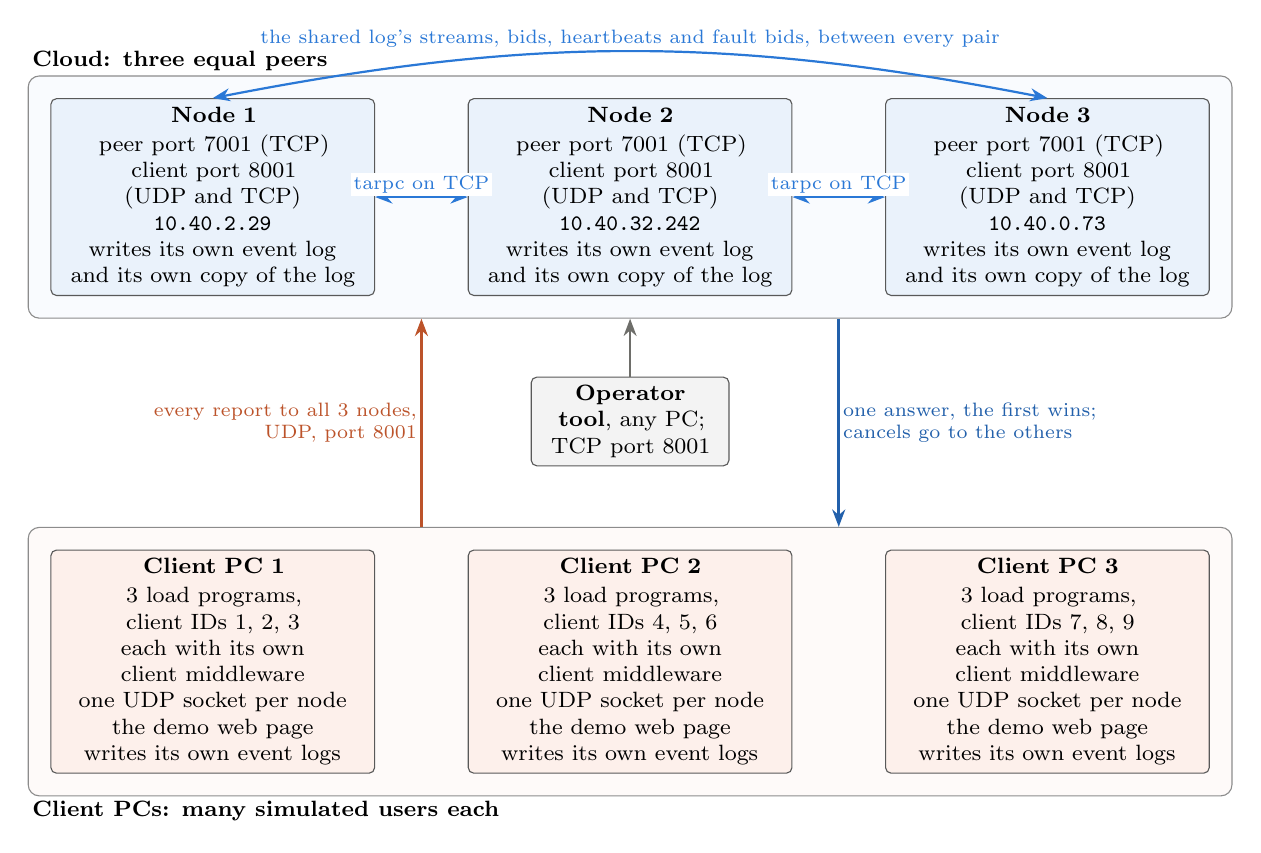
\begin{tikzpicture}[x=1cm,y=1cm]
  % Cloud nodes
  \foreach \i/\x/\ip in {1/0/10.40.2.29, 2/5.3/10.40.32.242, 3/10.6/10.40.0.73} {
    \node[nodebox, text width=3.9cm] (n\i) at (\x,0) {\textbf{Node \i}\\[1pt] peer port 7001 (TCP)\\ client port 8001 (UDP and TCP)\\ \texttt{\ip}\\ writes its own event log\\ and its own copy of the log};
  }
  \draw[<->, thick, nodeblue] (n1) -- node[elabel, above]{tarpc on TCP} (n2);
  \draw[<->, thick, nodeblue] (n2) -- node[elabel, above]{tarpc on TCP} (n3);
  \draw[<->, thick, nodeblue] (n1.north) to[bend left=11] node[elabel, above]{the shared log's streams, bids, heartbeats and fault bids, between every pair} (n3.north);
  \begin{scope}[on background layer]
    \node[group, fill=nodeblue!3, fit=(n1)(n3), inner sep=8pt, label={[grouplabel]north west:Cloud: three equal peers}] (cloud) {};
  \end{scope}
  % Client PCs
  \foreach \i/\x/\ids in {1/0/{1, 2, 3}, 2/5.3/{4, 5, 6}, 3/10.6/{7, 8, 9}} {
    \node[clientbox, text width=3.9cm] (c\i) at (\x,-5.9) {\textbf{Client PC \i}\\[1pt] 3 load programs, client IDs \ids\\ each with its own client middleware\\ one UDP socket per node\\ the demo web page\\ writes its own event logs};
  }
  \begin{scope}[on background layer]
    \node[group, fill=clientorange!3, fit=(c1)(c3), inner sep=8pt, label={[grouplabel, anchor=north west]south west:Client PCs: many simulated users each}] (clients) {};
  \end{scope}
  \draw[->, very thick, clientorange!80!black] ($(clients.north)+(-2.65,0)$) -- node[elabel, left, align=right]{every report to all 3 nodes,\\UDP, port 8001} ($(cloud.south)+(-2.65,0)$);
  \draw[->, very thick, nodeblue!80!black] ($(cloud.south)+(2.65,0)$) -- node[elabel, right, align=left]{one answer, the first wins;\\ cancels go to the others} ($(clients.north)+(2.65,0)$);
  \node[box, fill=libgray!10, text width=2.3cm] (ctl) at (5.3,-2.85) {\textbf{Operator tool}, any PC; TCP port 8001};
  \draw[->, semithick, libgray!80!black] (ctl.north) -- (ctl.north |- cloud.south);
\end{tikzpicture}
\caption{Deployment. The same node program runs on each cloud PC, and the same load programs on each client PC. The IP addresses are the ones in the final logs. In the experiments each client PC ran 3 load programs, so 9 in all; by default the start script starts 10 per PC.}
\label{fig:deploy}
\end{figure}

Client PCs reach each node on port 8001: reports go over UDP, and the operator tool and the web page's status checks go over TCP on the same port number. Nodes reach each other on port 7001 over TCP. Adding load changes no logic, because more programs or a higher rate are all it takes.

\subsection{Architectural model: the parts of a node}
\label{sec:components}

A cloud node is one process with no special role: the three nodes run the same program, and any of them can do any job. Figure~\ref{fig:components} shows its parts in three layers, and Table~\ref{tab:modules} gives the job of each.

\begin{itemize}
  \item \textbf{The application} is what the service does. The incident service takes a report, asks the middleware who should plan it, plans it if this node won, records the result, and replies. The planner picks the responder. The state machine holds the responders and the results, and changes them only in the order of the shared log. Responder release frees a responder when its job ends.
  \item \textbf{The cloud middleware} is how the nodes reach each other and survive failures. The bidding election picks the node that plans each report. The failure detector and the cloud group track who is alive. Takeover, the rejoin gate and degraded mode handle a node that goes quiet, comes back, or is left alone. The fault election picks the node that fails next. The worker pool runs plans off the async runtime. The shared log puts every change in one order on all three nodes.
  \item \textbf{The transport} carries the messages. Calls between nodes go over TCP and calls from clients over UDP, both through tarpc, with the team's own framing, datagram adapter and compression underneath.
\end{itemize}

The application never calls the transport or the shared log directly. It reaches the middleware through one narrow interface, and a test fails if it reaches past it (Section~\ref{sec:layers}). Arrows in Figure~\ref{fig:components} point from a part to the part it uses.

\begin{figure}[H]
\centering
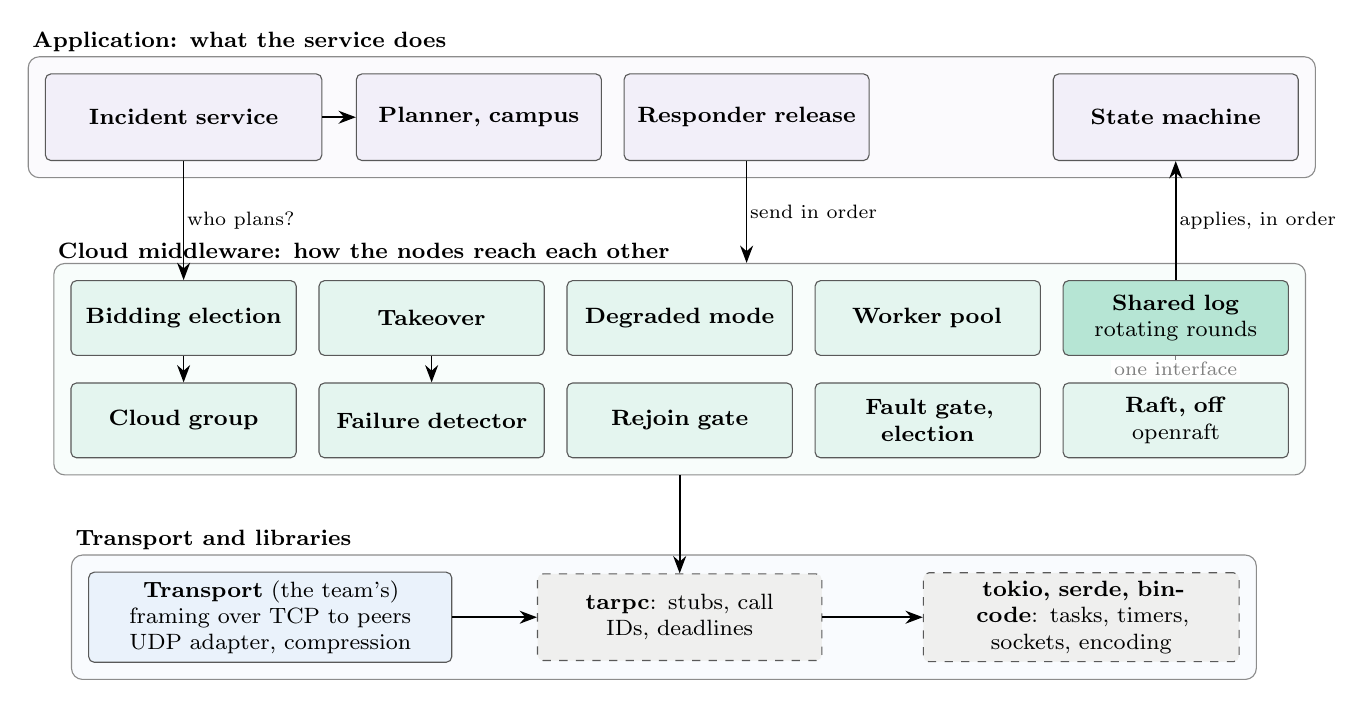
\begin{tikzpicture}[x=1cm,y=1cm, every node/.style={font=\scriptsize}]
  % Application, row 1
  \node[appbox, text width=3.3cm, minimum height=1.1cm] (svc) at (0,0) {\textbf{Incident service}};
  \node[appbox, text width=2.9cm, minimum height=1.1cm] (plan) at (3.75,0) {\textbf{Planner, campus}};
  \node[appbox, text width=2.9cm, minimum height=1.1cm] (rel) at (7.15,0) {\textbf{Responder release}};
  \node[appbox, text width=2.9cm, minimum height=1.1cm] (state) at (12.6,0) {\textbf{State machine}};
  \begin{scope}[on background layer]
    \node[group, fill=apppurple!3, fit=(svc)(state), label={[grouplabel]north west:Application: what the service does}] (appL) {};
  \end{scope}
  % Middleware, rows 2 and 3
  \foreach \n/\x/\t/\f in {bid/0/{\textbf{Bidding election}}/mwgreen!12,
                          take/3.15/{\textbf{Takeover}}/mwgreen!12,
                          deg/6.3/{\textbf{Degraded mode}}/mwgreen!12,
                          work/9.45/{\textbf{Worker pool}}/mwgreen!12,
                          log/12.6/{\textbf{Shared log}\\ rotating rounds}/mwgreen!32} {
    \node[mwbox, fill=\f, text width=2.65cm, minimum height=0.95cm] (\n) at (\x,-2.55) {\t};
  }
  \foreach \n/\x/\t in {grp/0/{\textbf{Cloud group}},
                       hb/3.15/{\textbf{Failure detector}},
                       rej/6.3/{\textbf{Rejoin gate}},
                       flt/9.45/{\textbf{Fault gate, election}},
                       raft/12.6/{\textbf{Raft, off}\\ openraft}} {
    \node[mwbox, text width=2.65cm, minimum height=0.95cm] (\n) at (\x,-3.85) {\t};
  }
  \begin{scope}[on background layer]
    \node[group, fill=mwgreen!3, fit=(bid)(raft), label={[grouplabel]north west:Cloud middleware: how the nodes reach each other}] (mwL) {};
  \end{scope}
  % Transport, row 4
  \node[nodebox, text width=4.4cm, minimum height=1.1cm] (tr) at (1.1,-6.35) {\textbf{Transport} (the team's)\\ framing over TCP to peers\\ UDP adapter, compression};
  \node[libbox, text width=3.4cm, minimum height=1.1cm] (tarpc) at (6.3,-6.35) {\textbf{tarpc}: stubs, call IDs, deadlines};
  \node[libbox, text width=3.8cm, minimum height=1.1cm] (tokio) at (11.4,-6.35) {\textbf{tokio, serde, bincode}: tasks, timers, sockets, encoding};
  \begin{scope}[on background layer]
    \node[group, fill=nodeblue!3, fit=(tr)(tokio), label={[grouplabel]north west:Transport and libraries}] (trL) {};
  \end{scope}
  % Arrows: within a row, and between layers
  \draw[flow] (svc) -- (plan);
  \draw[flow] (log.north) -- node[elabel, right]{applies, in order} (state.south);
  \draw[flow] (svc.south) -- node[elabel, right]{who plans?} (bid.north);
  \draw[flow] (rel.south) -- node[elabel, right]{send in order} (rel.south |- mwL.north);
  \draw[flow] (bid) -- (grp);
  \draw[flow] (take) -- (hb);
  \draw[densely dashed, black!50] (log) -- node[elabel]{one interface} (raft);
  \draw[flow] (mwL.south -| tarpc) -- (tarpc.north);
  \draw[flow] (tr) -- (tarpc);
  \draw[flow] (tarpc) -- (tokio);
\end{tikzpicture}
\caption{Inside one cloud node. Purple parts are the application, green parts the middleware, and grey dashed boxes libraries. The application reaches the middleware only through one interface. The shared log is rotating rounds in every lab run; Raft is kept behind the same interface (Section~\ref{sec:consensus-trait}). Every part writes events to the node's event log, and all share one node context.}
\label{fig:components}
\end{figure}

\begin{table}[!htb]
\centering\small
\caption{The parts of a node and of a client PC, and the job of each.}
\label{tab:modules}
\begin{tabularx}{\linewidth}{@{}P{4.2cm}L@{}}
\toprule
Part & Job \\
\midrule
Incident service & Takes a report, bids, plans if it wins, records the plan, replies \\
Bidding election & The election for each report (Section~\ref{sec:bidding}) \\
Planner & Picks a responder and a priority; makes the made-up campus \\
Worker pool & Runs plans off the async runtime, with a bounded queue \\
Shared log & One order for all commands, with no leader (Section~\ref{sec:sharedlog}) \\
Raft, kept but off & openraft behind the same interface (Section~\ref{sec:raft}) \\
State machine & Results and responder holds, the same on every node \\
Failure detector, group & Suspects a quiet peer; keeps this node's view of who is in \\
Takeover, release & Plans a report whose winner went quiet; frees responders \\
Fault gate and election & Elects the node that fails, and silences it \\
Rejoin, degraded mode & Stops serving until current; answers alone \\
Transport & TCP between nodes, UDP from clients, compression \\
Client middleware & Sends to all nodes, retries, keeps the first answer \\
Load programs and web page & Simulated users, and a small web page for the demo \\
Operator tool & Status, silence and slowdown of a node \\
\bottomrule
\end{tabularx}
\end{table}

\subsection{Application and middleware, on both sides}
\label{sec:layers}

The application and the middleware are kept apart: the application sends a message once, and the middleware makes sure the replicas get it. The line runs through both sides, as Figure~\ref{fig:layers} shows. On a client PC, a user submits a report with one call and names no node. The client middleware copies the report to all three nodes, resends it with the same ID if no answer comes, and keeps the first answer. On a node, the incident service asks the middleware who plans this report, and hands a result to it with one call, without knowing how the result reaches the other nodes. The middleware offers the application one narrow interface, and an automated test fails if application code reaches past it.

\begin{figure}[!htb]
\centering
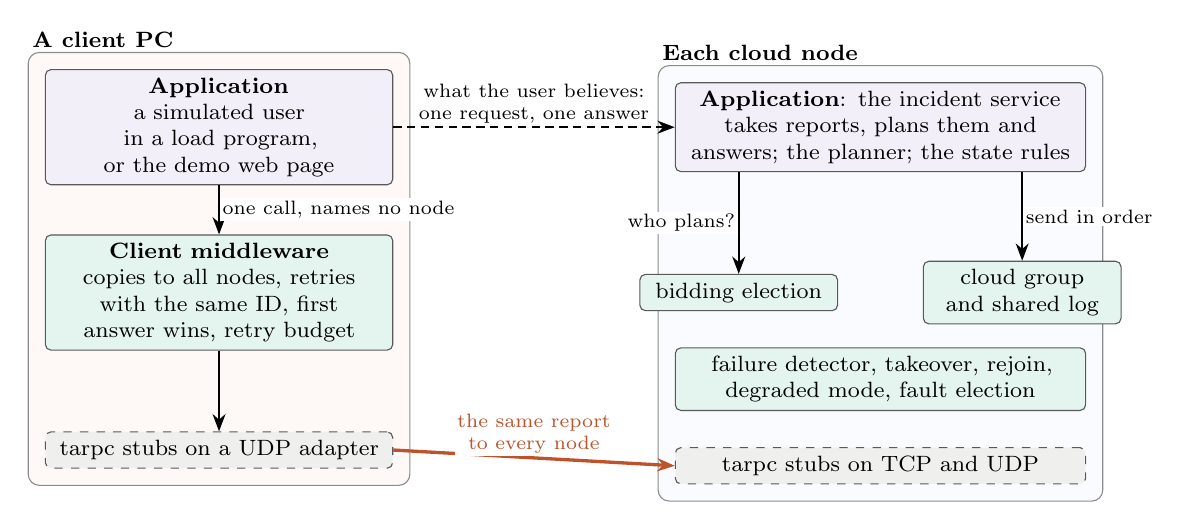
\begin{tikzpicture}[x=1cm,y=1cm]
  % Client side
  \node[appbox, text width=4.2cm] (user) at (0,0) {\textbf{Application}\\ a simulated user in a load program,\\ or the demo web page};
  \node[mwbox, text width=4.2cm] (mesh) at (0,-2.1) {\textbf{Client middleware}\\ copies to all nodes, retries with the same ID, first answer wins, retry budget};
  \node[libbox, text width=4.2cm] (crpc) at (0,-4.1) {tarpc stubs on a UDP adapter};
  \draw[flow] (user) -- node[elabel, right]{one call, names no node} (mesh);
  \draw[flow] (mesh) -- (crpc);
  \begin{scope}[on background layer]
    \node[group, fill=clientorange!4, fit=(user)(crpc), label={[grouplabel]north west:A client PC}] {};
  \end{scope}
  % Node side
  \node[appbox, text width=5.0cm] (svc) at (8.4,0) {\textbf{Application}: the incident service\\ takes reports, plans them and answers; the planner; the state rules};
  \node[mwbox, text width=2.3cm] (el) at (6.6,-2.1) {bidding election};
  \node[mwbox, text width=2.3cm] (gr) at (10.2,-2.1) {cloud group and shared log};
  \node[mwbox, text width=5.0cm] (ft) at (8.4,-3.2) {failure detector, takeover, rejoin, degraded mode, fault election};
  \node[libbox, text width=5.0cm] (nrpc) at (8.4,-4.3) {tarpc stubs on TCP and UDP};
  \draw[flow] (svc.south -| el.north) -- node[elabel, left]{who plans?} (el.north);
  \draw[flow] (svc.south -| gr.north) -- node[elabel, right]{send in order} (gr.north);
  \begin{scope}[on background layer]
    \node[group, fill=nodeblue!3, fit=(svc)(nrpc), label={[grouplabel]north west:Each cloud node}] (nodeside) {};
  \end{scope}
  \draw[->, very thick, clientorange!80!black] (crpc.east) -- node[elabel, above, align=center]{the same report\\to every node} (nrpc.west);
  \draw[dflow] (user.east) -- node[elabel, above, align=center]{what the user believes:\\ one request, one answer} (svc.west);
\end{tikzpicture}
\caption{The line between application and middleware runs through every client PC and every node. The dashed arrow is what the application sees; the solid arrow is what really happens.}
\label{fig:layers}
\end{figure}

\subsection{Peers, not client and server}
\label{sec:peers}

A client-server system fixes each machine's role for its whole life, and the RescueMesh cloud is not one. Its nodes send and receive requests at the same time: they share work, tell each other their load, check that each other is alive, and copy each other's log. So ``client'' and ``server'' are the roles of one call, not of a machine. When node 1 sends its bid to node 2, node 1 is the client for that call. A moment later node 2 sends its bid to node 1 and the roles swap. Table~\ref{tab:roles} lists the calls.

\begin{table}[!htb]
\centering\small
\caption{Who is client and who is server, per call.}
\label{tab:roles}
\begin{tabularx}{\linewidth}{@{}P{3.6cm}P{3.6cm}L@{}}
\toprule
Call & Client for this call & Server for this call \\
\midrule
A report & a client PC's middleware & whichever node answers first \\
A bid & the node that received the report & every peer in its view \\
A shared log stream & every node, for its own batches & every other member \\
A heartbeat & every node & every configured peer \\
A fault bid & every node that may bid & every peer in its view \\
A catch-up after a fault & the returning node & any member \\
Status, silence, slowdown & the operator tool or the web page & one node \\
\bottomrule
\end{tabularx}
\end{table}

\textbf{Who decides what.} No node decides for another. The node that plans a report is elected by all serving nodes from their bids. Whether a plan stands is decided by the same rule on every node, applied to the same log. Whether a peer is alive is decided by each node for itself. Which node fails next is decided by all three in a draw. Since Raft was removed, no node orders the log for the others either: the order is a sort that every node does by itself (Section~\ref{sec:sharedlog}).

\subsection{Fundamental model: failures and security}
\label{sec:fundamental}

\textbf{Failures.} The system handles these faults. A node can go silent: it ignores all traffic for 1 to 20 s and keeps its memory, which is the omission failure the spec requires to be injected. A node's process can die and restart, which loses its memory; the experiments use \texttt{kill -9} for this, and a kill stands in for turning a machine off. Two or all three nodes can fail together or one after the other. Messages can be lost, late or duplicated, above all over UDP. The system does not handle a node that lies or sends wrong data (Byzantine failure), or a long split of the network in which a client can reach no serving node.

These faults shape the design in three ways. Every failure detector in the system is a timer, and a timer cannot tell a slow node from a dead one \cite{chandra}. So a wrong guess must be cheap: it may cost repeated work, but never two results for one report. A restart wipes memory, so each node saves what it applied to its own disk before it answers. And a client must never need to know which node failed, so it always sends to all three.

\textbf{Security.} All data is synthetic, and Phase 1 has no security requirements. Nodes trust each other and trust what clients send. The web page listens only on its own PC, with no password.

\subsection{Data model}
\label{sec:datamodel}

Figure~\ref{fig:uml-data} is the UML class diagram of the replicated state. Every node holds one copy of the cloud state, and only the state machine changes it, in log order. Every number in it is an integer, so that every node computes exactly the same thing. Its tables are sorted maps, never hash maps, so that their order is the same on every node.

\begin{figure}[!htb]
\centering
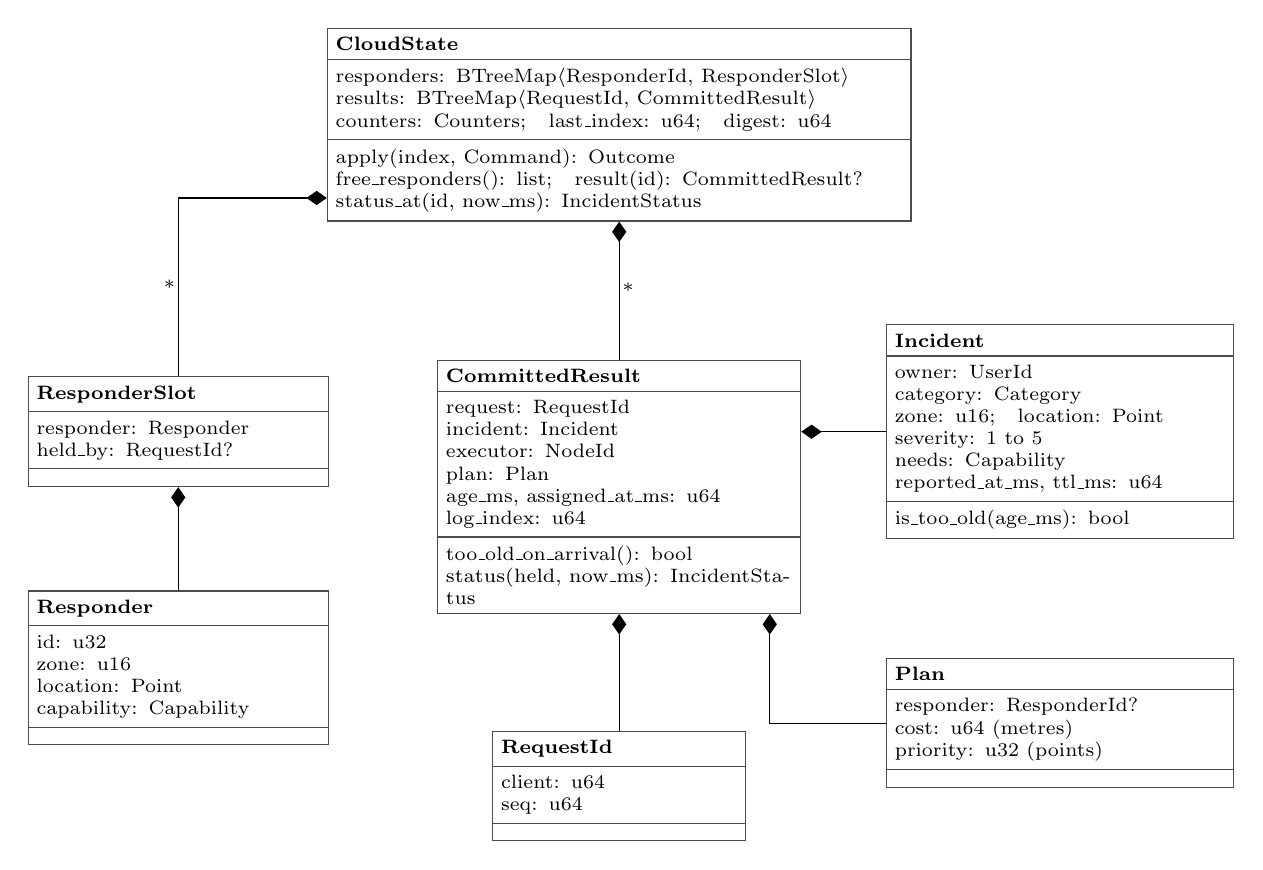
\begin{tikzpicture}[x=1cm,y=1cm]
  \node[umlclass=7.2cm] (cs) at (0,0) {\textbf{CloudState}
    \nodepart{two} responders: BTreeMap$\langle$ResponderId, ResponderSlot$\rangle$\\ results: BTreeMap$\langle$RequestId, CommittedResult$\rangle$\\ counters: Counters;\quad last\_index: u64;\quad digest: u64
    \nodepart{three} apply(index, Command): Outcome\\ free\_responders(): list;\quad result(id): CommittedResult?\\ status\_at(id, now\_ms): IncidentStatus};
  \node[umlclass=3.6cm] (slot) at (-5.6,-3.9) {\textbf{ResponderSlot}
    \nodepart{two} responder: Responder\\ held\_by: RequestId?
    \nodepart{three} };
  \node[umlclass=3.6cm] (resp) at (-5.6,-6.9) {\textbf{Responder}
    \nodepart{two} id: u32\\ zone: u16\\ location: Point\\ capability: Capability
    \nodepart{three} };
  \node[umlclass=4.4cm] (cr) at (0,-4.6) {\textbf{CommittedResult}
    \nodepart{two} request: RequestId\\ incident: Incident\\ executor: NodeId\\ plan: Plan\\ age\_ms, assigned\_at\_ms: u64\\ log\_index: u64
    \nodepart{three} too\_old\_on\_arrival(): bool\\ status(held, now\_ms): IncidentStatus};
  \node[umlclass=4.2cm] (inc) at (5.6,-3.9) {\textbf{Incident}
    \nodepart{two} owner: UserId\\ category: Category\\ zone: u16;\quad location: Point\\ severity: 1 to 5\\ needs: Capability\\ reported\_at\_ms, ttl\_ms: u64
    \nodepart{three} is\_too\_old(age\_ms): bool};
  \node[umlclass=4.2cm] (plan) at (5.6,-7.6) {\textbf{Plan}
    \nodepart{two} responder: ResponderId?\\ cost: u64 (metres)\\ priority: u32 (points)
    \nodepart{three} };
  \node[umlclass=3.0cm] (rid) at (0,-8.4) {\textbf{RequestId}
    \nodepart{two} client: u64\\ seq: u64
    \nodepart{three} };
  \draw[compose] (slot.north) |- node[elabel, pos=0.25, left]{*} ($(cs.south west)+(0,0.3)$);
  \draw[compose] (cr.north) -- node[elabel, right]{*} (cs.south);
  \draw[compose] (resp.north) -- (slot.south);
  \draw[compose] (inc.west) -- (inc.west -| cr.east);
  \draw[compose] (plan.west) -| ($(cr.south east)+(-0.4,0)$);
  \draw[compose] (rid.north) -- (cr.south);
\end{tikzpicture}
\caption{UML class diagram of the replicated state. A filled diamond means the whole owns the part. A ``?'' marks an optional field. An incident's status is never stored: it is worked out on read from the record and the hold.}
\label{fig:uml-data}
\end{figure}

Three commands change the state, and each is safe to apply twice: \emph{register responders} adds the campus's responders, \emph{commit result} records the plan for one report, and \emph{release responder} frees a responder when its job ends. The first result committed for a report ID wins on every node, and any later one is marked a duplicate and gets the winner back. A plan whose responder another report took in the meantime is \emph{stale}. In the final build it is chosen again at apply, the same way on every node. Figure~\ref{fig:apply} draws the rule.

\begin{figure}[!htb]
\centering
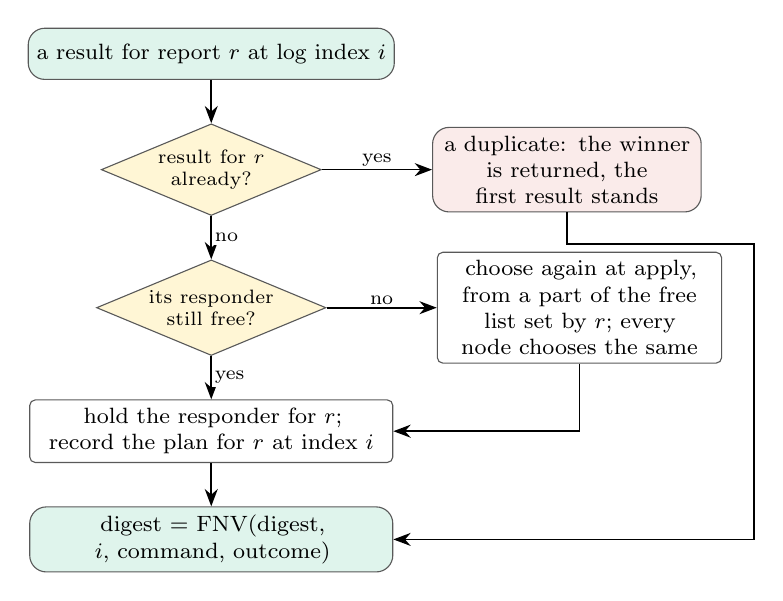
\begin{tikzpicture}[x=1cm,y=1cm, node distance=0.55cm]
  \node[fend] (start) {a result for report $r$ at log index $i$};
  \node[fdec, below=of start] (have) {result for $r$\\already?};
  \node[fbad, right=1.4cm of have, text width=3.2cm] (dup) {a duplicate: the winner\\ is returned, the first result stands};
  \node[fdec, below=of have] (free) {its responder\\still free?};
  \node[fstep, right=1.4cm of free, text width=3.4cm] (again) {choose again at apply, from a part of the free list set by $r$; every node chooses the same};
  \node[fstep, below=of free, text width=4.4cm] (hold) {hold the responder for $r$;\\ record the plan for $r$ at index $i$};
  \node[fend, below=of hold, text width=4.4cm] (dig) {digest = FNV(digest, $i$, command, outcome)};
  \draw[flow] (start) -- (have);
  \draw[flow] (have) -- node[elabel, above]{yes} (dup);
  \draw[flow] (have) -- node[elabel, right]{no} (free);
  \draw[flow] (free) -- node[elabel, above]{no} (again);
  \draw[flow] (free) -- node[elabel, right]{yes} (hold);
  \draw[flow] (again.south) |- (hold.east);
  \draw[flow] (hold) -- (dig);
  \draw[flow] (dup.south) -- ++(0,-0.4) -| ($(again.east)+(0.4,0)$) |- (dig.east);
\end{tikzpicture}
\caption{How every node applies one result. No clock, no network and no randomness is read here, so every node reaches the same state and the same digest.}
\label{fig:apply}
\end{figure}

\textbf{The digest.} After each command, every node computes a new digest from the old one, the log index, the command and its outcome. One different command, order or outcome changes every digest after it. Each node logs its digest at every 100th log index, and comparing these checkpoints across nodes shows whether the copies agree.

\subsection{One interface, two shared logs}
\label{sec:consensus-trait}

The most useful design choice for this phase turned out to be an interface. From the start, every part of the node reached the shared log only through one interface, \emph{Consensus}, and never called Raft directly. When Raft had to be replaced (Section~\ref{sec:raft}), the new shared log was written as a second implementation of the same interface, and one setting in the config file chooses between them. Nothing above the interface changed: not the bidding, the planner, the state machine, the replies or the digests. That is also why both designs still build, and why the Raft tests still pass (Section~\ref{sec:tests}). Figure~\ref{fig:uml-consensus} shows the classes.

\begin{figure}[!htb]
\centering
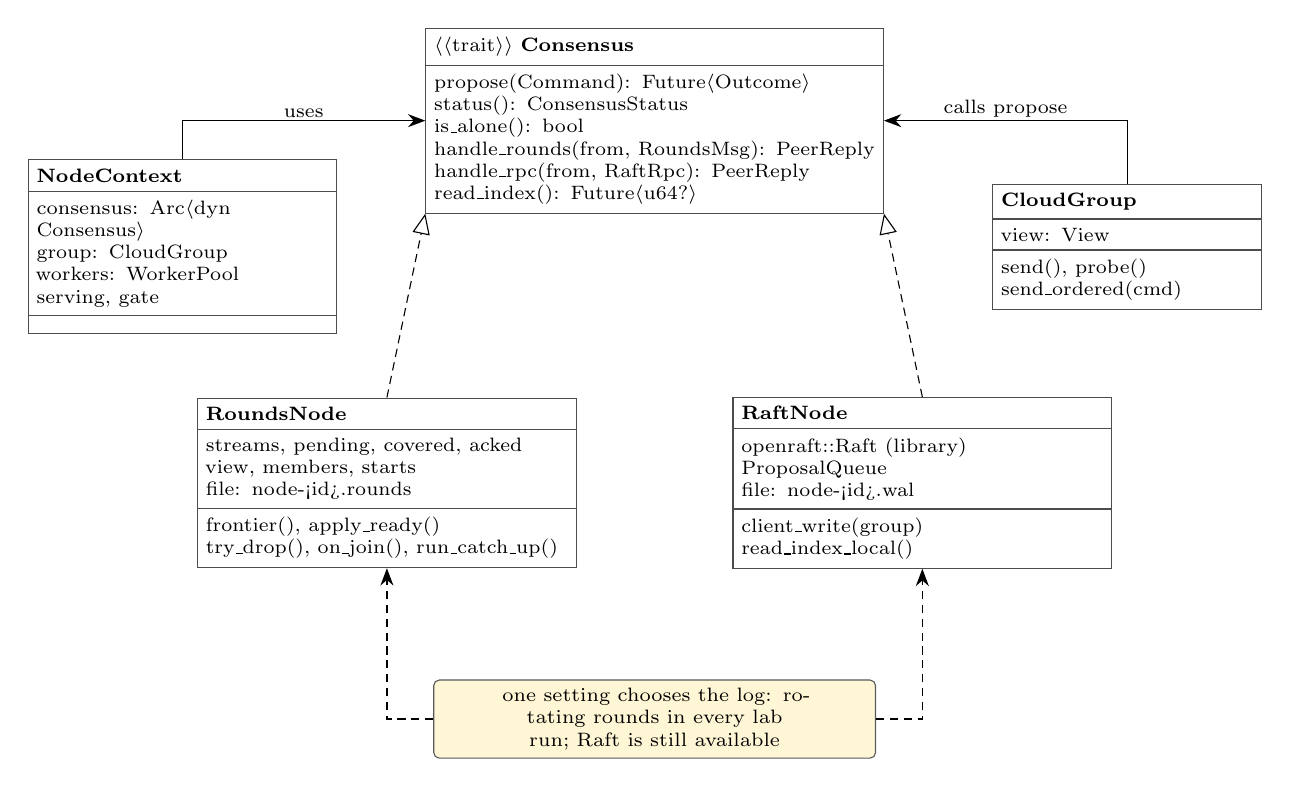
\begin{tikzpicture}[x=1cm,y=1cm]
  \node[umliface=5.6cm] (tr) at (0,0) {$\langle\langle$trait$\rangle\rangle$ \textbf{Consensus}
    \nodepart{two} propose(Command): Future$\langle$Outcome$\rangle$\\ status(): ConsensusStatus\\ is\_alone(): bool\\ handle\_rounds(from, RoundsMsg): PeerReply\\ handle\_rpc(from, RaftRpc): PeerReply\\ read\_index(): Future$\langle$u64?$\rangle$};
  \node[umlclass=4.6cm] (rn) at (-3.4,-4.6) {\textbf{RoundsNode}
    \nodepart{two} streams, pending, covered, acked\\ view, members, starts\\ file: node-<id>.rounds
    \nodepart{three} frontier(), apply\_ready()\\ try\_drop(), on\_join(), run\_catch\_up()};
  \node[umlclass=4.6cm] (rf) at (3.4,-4.6) {\textbf{RaftNode}
    \nodepart{two} openraft::Raft (library)\\ ProposalQueue\\ file: node-<id>.wal
    \nodepart{three} client\_write(group)\\ read\_index\_local()};
  \node[umlclass=3.7cm] (ctx) at (-6.0,-1.6) {\textbf{NodeContext}
    \nodepart{two} consensus: Arc$\langle$dyn Consensus$\rangle$\\ group: CloudGroup\\ workers: WorkerPool\\ serving, gate
    \nodepart{three} };
  \node[umlclass=3.2cm] (grp) at (6.0,-1.6) {\textbf{CloudGroup}
    \nodepart{two} view: View
    \nodepart{three} send(), probe()\\ send\_ordered(cmd)};
  \node[box, fill=notefill, text width=5.4cm, font=\scriptsize] (cfg) at (0,-7.6) {one setting chooses the log: rotating rounds in every lab run; Raft is still available};
  \draw[realize] (rn.north) -- (tr.south west);
  \draw[realize] (rf.north) -- (tr.south east);
  \draw[assoc] (ctx.north) |- node[elabel, above, pos=0.75]{uses} (tr.west);
  \draw[assoc] (grp.north) |- node[elabel, above, pos=0.75]{calls propose} (tr.east);
  \draw[dflow] (cfg.west) -| (rn.south);
  \draw[dflow] (cfg.east) -| (rf.south);
\end{tikzpicture}
\caption{UML class diagram of the shared log's interface. A dashed arrow with an open triangle means ``implements''. The rest of the node sees only the interface, so it cannot tell which log is underneath.}
\label{fig:uml-consensus}
\end{figure}

% ==============================================================================================
\section{Parallelization, workload and planner}
\label{sec:conc}

The spec requires concurrent request processing and a documented parallel model on both the client and the cloud side. A node is busy in three ways at once: it receives reports from clients, it plans them, and it talks to its peers. These must not hold each other up.

\subsection{Inside a cloud node}

A node runs on tokio, a Rust runtime that runs many small tasks on a few threads. Every client call, every peer call and every report gets its own task (\dlog{D47}). Planning is CPU work, so it does not run on the runtime. It runs on a separate pool of plain threads with a bounded queue: 20 threads and a queue of 4,096 jobs in the lab (\dlog{D48}, \dlog{D71}). When the pool is full, the node refuses the job, logs \texttt{overloaded}, and stays quiet, and the client's retry goes to the nodes again (\dlog{D36}). A node that already holds 16,000 reports in progress refuses new ones at the door in the same way (\dlog{D250}, \dlog{D253}). Figure~\ref{fig:node-conc} shows the tasks and how they meet.

\begin{figure}[!htb]
\centering
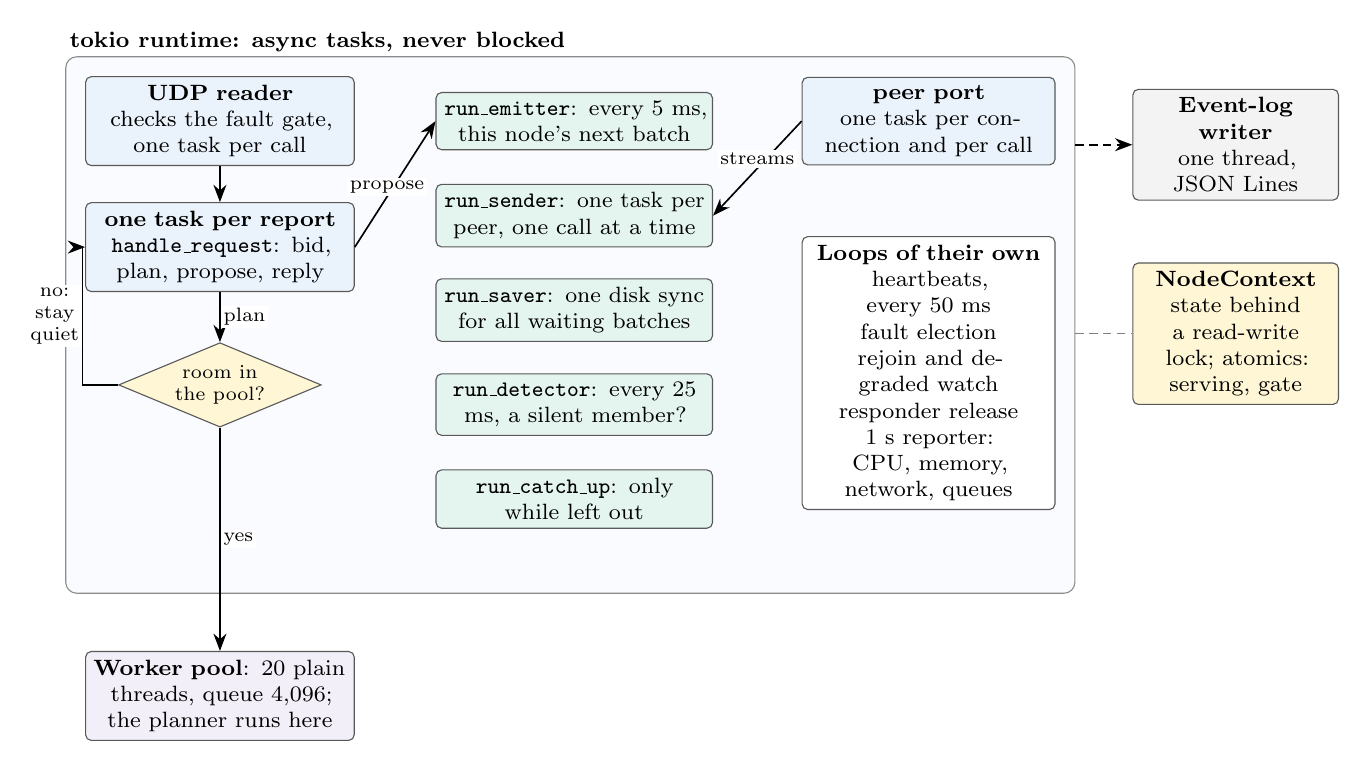
\begin{tikzpicture}[x=1cm,y=1cm, every node/.style={font=\scriptsize}]
  % Left column: requests from clients
  \node[nodebox, text width=3.2cm] (udp) at (0,0) {\textbf{UDP reader}\\ checks the fault gate,\\ one task per call};
  \node[nodebox, text width=3.2cm] (rep) at (0,-1.6) {\textbf{one task per report}\\ \texttt{handle\_request}: bid, plan, propose, reply};
  \node[fdec] (adm) at (0,-3.35) {room in\\ the pool?};
  \draw[flow] (udp) -- (rep);
  \draw[flow] (rep) -- node[elabel, right]{plan} (adm);
  \draw[flow] (adm.west) -- ++(-0.45,0) |- node[elabel, pos=0.25, left, align=center]{no:\\ stay\\ quiet} (rep.west);
  % Middle column: the shared log's tasks
  \node[mwbox, text width=3.3cm] (em) at (4.5,0) {\texttt{run\_emitter}: every 5 ms, this node's next batch};
  \node[mwbox, text width=3.3cm] (snd) at (4.5,-1.2) {\texttt{run\_sender}: one task per peer, one call at a time};
  \node[mwbox, text width=3.3cm] (sav) at (4.5,-2.4) {\texttt{run\_saver}: one disk sync for all waiting batches};
  \node[mwbox, text width=3.3cm] (det) at (4.5,-3.6) {\texttt{run\_detector}: every 25 ms, a silent member?};
  \node[mwbox, text width=3.3cm] (cat) at (4.5,-4.8) {\texttt{run\_catch\_up}: only while left out};
  \begin{scope}[on background layer]
    \node[group, fill=mwgreen!3, fit=(em)(cat), inner sep=4pt, label={[grouplabel, anchor=north]south:Shared log (\texttt{rounds.rs})}] (logg) {};
  \end{scope}
  \draw[flow] (rep.east) -- node[elabel, above, pos=0.4]{propose} (em.west);
  % Right column: peers and loops
  \node[nodebox, text width=3.0cm] (peer) at (9.0,0) {\textbf{peer port}\\ one task per connection and per call};
  \node[box, fill=white, text width=3.0cm] (loops) at (9.0,-3.2) {\textbf{Loops of their own}\\ heartbeats, every 50 ms\\ fault election\\ rejoin and degraded watch\\ responder release\\ 1 s reporter: CPU, memory, network, queues};
  \draw[flow] (peer.west) -- node[elabel, above]{streams} (snd.east);
  \coordinate (rtbottom) at (4.5,-5.75);
  \begin{scope}[on background layer]
    \node[group, fill=nodeblue!3, fit=(udp)(adm)(logg)(peer)(loops)(rtbottom), inner sep=7pt, label={[grouplabel]north west:tokio runtime: async tasks, never blocked}] (rt) {};
  \end{scope}
  % Outside the runtime
  \node[appbox, text width=3.2cm] (pool) at (0,-7.3) {\textbf{Worker pool}: 20 plain threads, queue 4,096; the planner runs here};
  \draw[flow] (adm.south) -- node[elabel, right]{yes} (pool.north);
  \node[box, fill=libgray!10, text width=2.4cm] (logw) at (12.9,-0.3) {\textbf{Event-log writer}\\ one thread, JSON Lines};
  \node[box, fill=notefill, text width=2.4cm] (ctx) at (12.9,-2.7) {\textbf{NodeContext}\\ state behind a read-write lock; atomics: serving, gate};
  \draw[dflow] (rt.east |- logw.west) -- (logw.west);
  \draw[densely dashed, black!50] (rt.east |- ctx.west) -- (ctx.west);
\end{tikzpicture}
\caption{Concurrency inside one node, at the final build. Planning is the only CPU-heavy work, and it never runs on the async runtime, so heartbeats and the shared log keep their timing however busy the node is.}
\label{fig:node-conc}
\end{figure}

A few rules keep this safe, and the build checks some of them (\dlog{D47}, \dlog{D66}). No task may block the runtime: no sleeping threads, and no blocking file or network calls. No lock may be held across a wait, which the linter denies. Every task is owned, so it ends when its owner or its channel does. Writing a log line goes through a channel to one writer thread, so it never holds up a request.

One rule came from the team's own experience rather than from the textbooks. In the lab rehearsal, saving to disk once crowded out the leader's heartbeats, and the cluster went through 225 elections in one run with no report answered (\dlog{D133}). The rule since then is that saving to disk and the ``I am alive'' message of a node come first, and processing requests can never crowd them out. In the final build the heartbeats run on their own loop, the shared log saves every waiting batch with one disk sync, and planning can only fill the worker pool.

\subsection{On a client PC}

A client PC runs several real operating-system programs, \texttt{loadgen}, and each simulated user is a tokio task inside one of them (\dlog{D181}). All users of one program share one client middleware, \code{MeshClient}, with one UDP socket per node. Figure~\ref{fig:client-conc} shows the shape. One script, \texttt{scripts/start-users.sh}, starts and stops a PC's programs, gives each a unique client ID from the PC's number, and adds up their totals at the end (\dlog{D183}, \dlog{D184}). By default it starts 10 programs per PC; the experiments here used 3 per PC.

\begin{figure}[!htb]
\centering
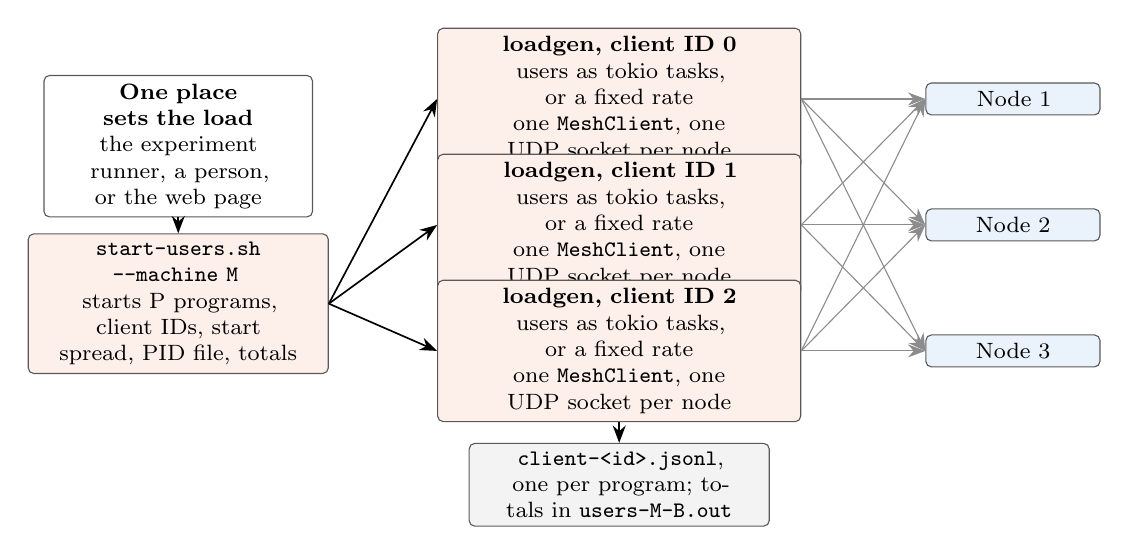
\begin{tikzpicture}[x=1cm,y=1cm, every node/.style={font=\scriptsize}]
  \node[box, fill=white, text width=3.2cm] (who) at (0,0) {\textbf{One place sets the load}\\ the experiment runner, a person, or the web page};
  \node[clientbox, text width=3.6cm] (script) at (0,-2.0) {\texttt{start-users.sh --machine M}\\ starts P programs, client IDs, start spread, PID file, totals};
  \foreach \k/\y in {0/0.6, 1/-1.0, 2/-2.6} {
    \node[clientbox, text width=4.4cm] (p\k) at (5.6,\y) {\textbf{loadgen, client ID \k}\\ users as tokio tasks, or a fixed rate\\ one \texttt{MeshClient}, one UDP socket per node};
  }
  \node[nodebox, text width=2.0cm] (n1) at (10.6,0.6) {Node 1};
  \node[nodebox, text width=2.0cm] (n2) at (10.6,-1.0) {Node 2};
  \node[nodebox, text width=2.0cm] (n3) at (10.6,-2.6) {Node 3};
  \node[box, fill=libgray!10, text width=3.6cm] (logs) at (5.6,-4.3) {\texttt{client-<id>.jsonl}, one per program; totals in \texttt{users-M-B.out}};
  \draw[flow] (who) -- (script);
  \foreach \k in {0,1,2} {
    \draw[flow] (script.east) -- (p\k.west);
    \foreach \n in {1,2,3} { \draw[->, thin, black!45] (p\k.east) -- (n\n.west); }
  }
  \draw[flow] (p2.south) -- (logs.north);
\end{tikzpicture}
\caption{A client PC. Every program sends every report to all three nodes, so the cloud sees each report three times and the user sees one answer.}
\label{fig:client-conc}
\end{figure}

\textbf{Closed and open loop.} A program can run two ways (\dlog{D54}). In a closed loop, each user sends a report, waits for the answer, waits a moment, and sends the next. This is how a person behaves, but a slow cloud slows its own users down, which hides the problem. In an open loop, a program sends at a fixed rate whatever happens, evenly spaced, and latency counts from when a report was due to go, so a queue in the load program is not hidden. The overnight series and the final runs use the open loop: 9 programs, 3 on each client PC, each with its own random seed. A program keeps at most 20,000 reports open and waits for a free place beyond that.

\subsection{The workload}

Each report is drawn uniformly at random (\texttt{campus.rs}, \dlog{D99}): a zone, a position in it, a severity from 1 to 5, a category from the spec's list of events, and the capability it needs, which the category decides (\dlog{D141}). Each report is valid for 60 s (\dlog{D143}). The campus has 60,000 responders in the speed and kill runs and 300 in the lab guide's tests, spread evenly over zones and capabilities. Choosing a responder holds it for 200 ms times the report's severity, so 0.2 to 1 s, and then it is released through the shared log (\dlog{D111}). Each report costs the log about 2.3 commands: the result, the release, and sometimes a duplicate when two nodes planned the same report.

\subsection{The planner}

The planner is deterministic, explainable and tunable, as the spec requires, and its cost can be raised to create real computing load. It takes the report, its age and the free responders as arguments, and reads no network, no clock and no randomness, so the same inputs give the same plan on any node (\dlog{D49}). Figure~\ref{fig:planner} shows how it picks.

\begin{figure}[!htb]
\centering
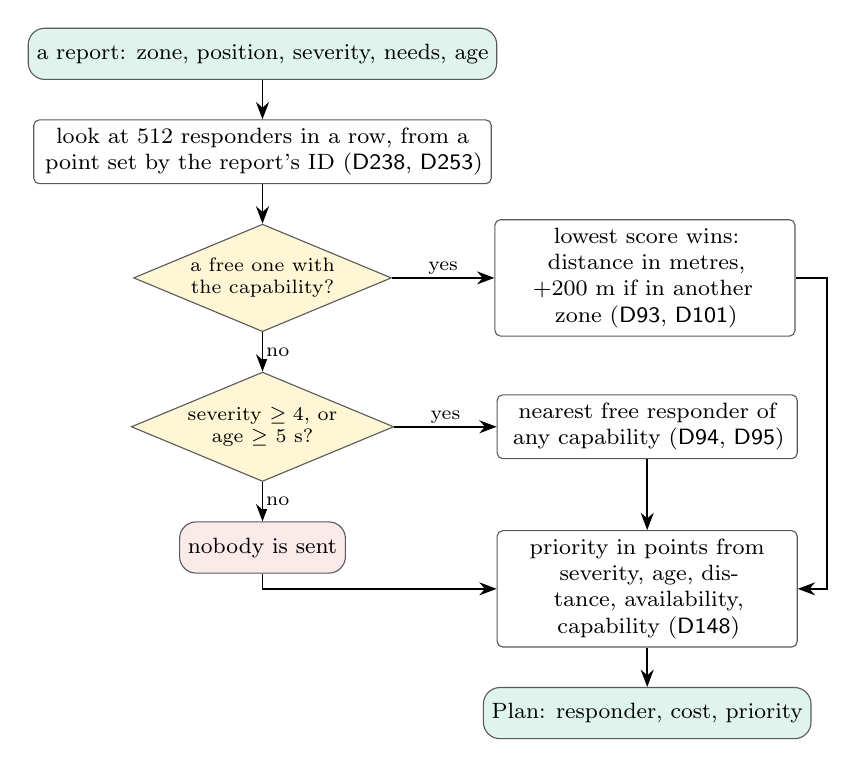
\begin{tikzpicture}[x=1cm,y=1cm, node distance=0.5cm]
  \node[fend] (s) {a report: zone, position, severity, needs, age};
  \node[fstep, below=of s, text width=5.6cm] (look) {look at 512 responders in a row, from a point set by the report's ID (\dlog{D238}, \dlog{D253})};
  \node[fdec, below=of look] (any) {a free one with\\ the capability?};
  \node[fstep, right=1.3cm of any, text width=3.6cm] (best) {lowest score wins:\\ distance in metres, +200 m if in another zone (\dlog{D93}, \dlog{D101})};
  \node[fdec, below=of any] (sev) {severity $\ge 4$, or\\ age $\ge$ 5 s?};
  \node[fstep, right=1.3cm of sev, text width=3.6cm] (fall) {nearest free responder of any capability (\dlog{D94}, \dlog{D95})};
  \node[fbad, below=of sev] (none) {nobody is sent};
  \node[fstep, below=0.9cm of fall, text width=3.6cm] (pri) {priority in points from severity, age, distance, availability, capability (\dlog{D148})};
  \node[fend, below=of pri] (plan) {Plan: responder, cost, priority};
  \draw[flow] (s) -- (look);
  \draw[flow] (look) -- (any);
  \draw[flow] (any) -- node[elabel, above]{yes} (best);
  \draw[flow] (any) -- node[elabel, right]{no} (sev);
  \draw[flow] (sev) -- node[elabel, above]{yes} (fall);
  \draw[flow] (sev) -- node[elabel, right]{no} (none);
  \draw[flow] (best.east) -- ++(0.4,0) |- (pri.east);
  \draw[flow] (fall) -- (pri);
  \draw[flow] (none) |- (pri.west);
  \draw[flow] (pri) -- (plan);
\end{tikzpicture}
\caption{The planner (\texttt{src/planner.rs}). If nobody free among the 512 has the capability, it looks at the whole table before falling back. Ties go to the same zone, then the lowest responder ID.}
\label{fig:planner}
\end{figure}

\textbf{Priority.} The priority says how urgent a report is, in whole points, and it never changes who is sent (\dlog{D148}). One step of severity is worth 100 points, and the other factors are measured against it: severity gives 100 to 500, age 1 point per 50 ms up to 400, distance 1 point per 10 m up to 100, availability $100/(\text{free}+1)$, and 100 more if no free responder has the needed capability. For example, a severity 4 report, 1 s old, with a matching responder 300 m away and 9 free, scores $400 + 20 + 30 + 10 + 0 = 460$.

\textbf{Tunable load.} Choosing the nearest responder is cheap, a few microseconds. The spec requires planning that creates real computing load, so a setting, \texttt{plan\_work}, adds a busy loop of integer mixing that never changes the plan (\dlog{D96}). Its cost, measured from the nodes' own bids overnight: with \texttt{plan\_work} 0 a plan takes about 8 $\mu$s, and with 1000 it takes 3.9 ms at the median and 4.7 ms at p99. Every result in this report states its \texttt{plan\_work}, because the two give very different ceilings.

% ==============================================================================================
\section{Protocols and message formats}
\label{sec:proto}

This section describes how the programs talk: the paths, the messages, the timers, the retries and how duplicates are handled. The full tables are in \texttt{docs/protocol.md} and \texttt{docs/shared-log.md} \cite{repo}.

\subsection{The life of one report}

The easiest way to see the protocol is to follow one real report. Figure~\ref{fig:seq-report} draws one report from a run at 10,000 reports a second, taken line by line from the event logs of all four PCs it touched (\texttt{analysis/results/request-trace-example.txt}). The times count from the client's send. They come from four different clocks, which were within a few milliseconds of each other, so they are close but not exact.

\begin{figure}[!htb]
\centering
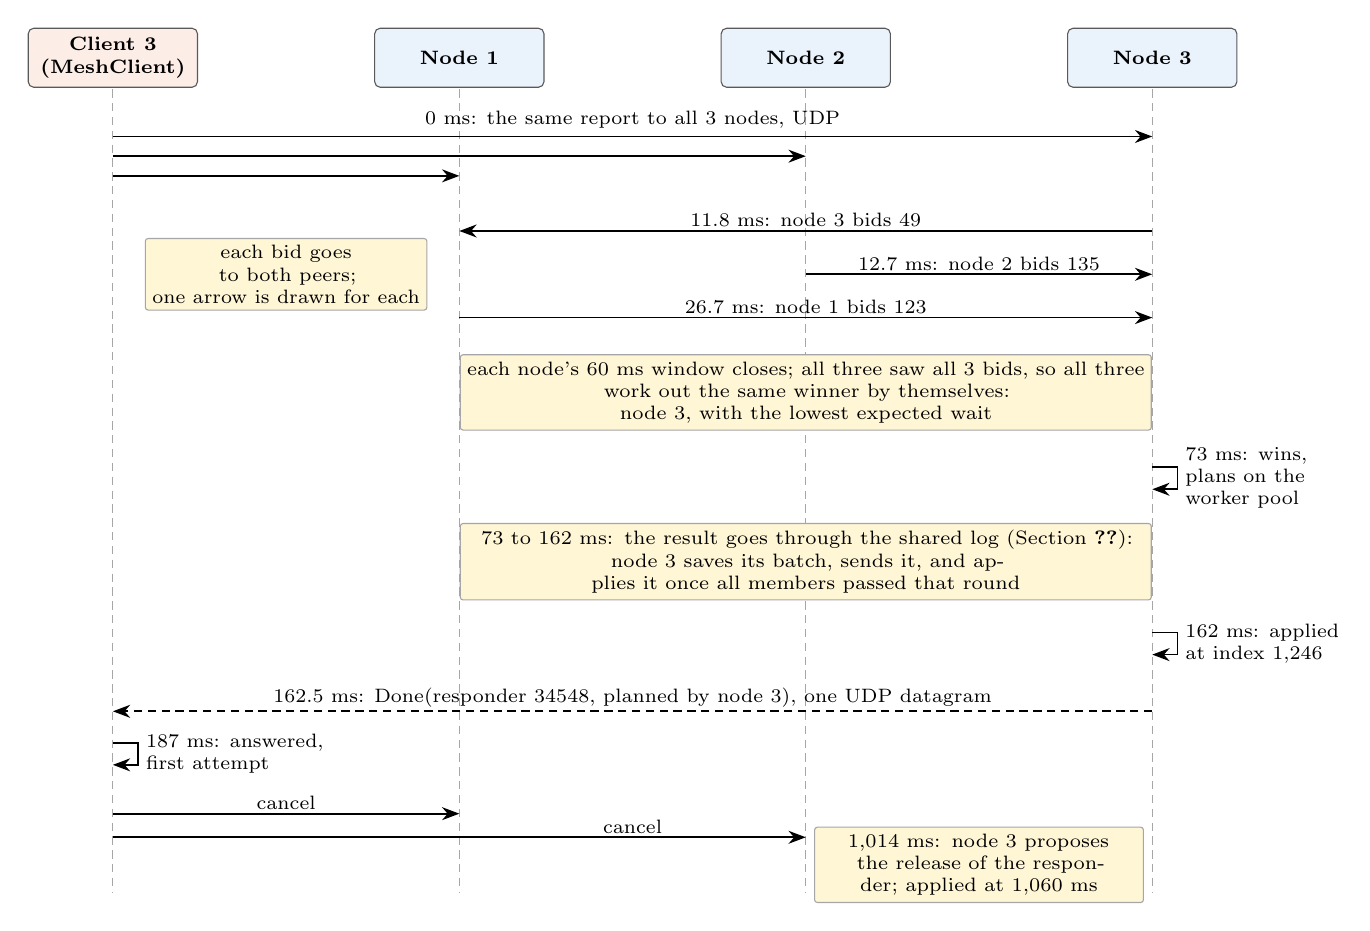
\begin{tikzpicture}[x=1cm,y=1cm]
  \seqactor[clientorange!12]{0}{Client 3\\(MeshClient)}{-10.6}
  \seqactor{4.4}{Node 1}{-10.6}
  \seqactor{8.8}{Node 2}{-10.6}
  \seqactor{13.2}{Node 3}{-10.6}
  % the group send
  \seqmsg{0}{13.2}{-1.0}{}
  \seqmsg{0}{8.8}{-1.25}{}
  \seqmsg{0}{4.4}{-1.5}{}
  \node[mlabel] at (6.6,-0.95) {0 ms: the same report to all 3 nodes, UDP};
  % bids
  \seqmsg{13.2}{4.4}{-2.2}{11.8 ms: node 3 bids 49}
  \seqmsg{8.8}{13.2}{-2.75}{12.7 ms: node 2 bids 135}
  \seqmsg{4.4}{13.2}{-3.3}{26.7 ms: node 1 bids 123}
  \seqnote{2.2}{-2.75}{3.4}{each bid goes to both peers;\\ one arrow is drawn for each}
  \seqnote{8.8}{-4.25}{8.6}{each node's 60 ms window closes; all three saw all 3 bids, so all three\\ work out the same winner by themselves: node 3, with the lowest expected wait}
  \seqself{13.2}{-5.2}{73 ms: wins,\\ plans on the\\ worker pool}
  \seqnote{8.8}{-6.4}{8.6}{73 to 162 ms: the result goes through the shared log (Section~\ref{sec:sharedlog}):\\ node 3 saves its batch, sends it, and applies it once all members passed that round}
  \seqself{13.2}{-7.3}{162 ms: applied\\ at index 1,246}
  \seqrep{13.2}{0}{-8.3}{162.5 ms: Done(responder 34548, planned by node 3), one UDP datagram}
  \seqself{0}{-8.7}{187 ms: answered,\\ first attempt}
  \seqmsg{0}{4.4}{-9.6}{cancel}
  \seqmsg{0}{8.8}{-9.9}{}
  \node[mlabel] at (6.6,-9.9) {cancel};
  \seqnote{11.0}{-10.25}{4.0}{1,014 ms: node 3 proposes the release of the responder; applied at 1,060 ms}
\end{tikzpicture}
\caption{One report at 10,000 a second, from the logs (\commit{eba4d14}, \texttt{plan\_work} 0). Nodes 1 and 2 lost the bid and stood by; they say nothing to the client unless the winner goes quiet. The client gets one answer and cancels its calls to the other two nodes.}
\label{fig:seq-report}
\end{figure}

\subsection{Paths and messages}

\begin{table}[!htb]
\centering\small
\caption{The paths between programs.}
\label{tab:paths}
\begin{tabularx}{\linewidth}{@{}P{3.4cm}P{3.6cm}L@{}}
\toprule
Path & Transport & What it carries \\
\midrule
Client to all 3 nodes & tarpc over UDP, port 8001 & \code{submit(ClientRequest)}, three copies with one ID; a cancel once answered \\
Node to client & the same socket & one \code{ClientReply}; the first one wins \\
Node to node & tarpc over TCP, port 7001; the shared log has its own connection (\dlog{D251}) & log streams, bids, heartbeats, fault bids, catch-up \\
\texttt{ctl} and web page to a node & tarpc over TCP, port 8001 & status, silence, slowdown, records; passes the fault gate \\
\bottomrule
\end{tabularx}
\end{table}

\begin{table}[!htb]
\centering\small
\caption{The main messages and records (\texttt{src/proto.rs}). Every number is an integer.}
\label{tab:messages}
\begin{tabularx}{\linewidth}{@{}P{3.5cm}L@{}}
\toprule
Message & Fields and meaning \\
\midrule
\code{ClientRequest} & \code{id} (client, seq), \code{attempt}, \code{age\_ms}, \code{incident}. A retry keeps the ID and raises \code{attempt}. \code{age\_ms} is how old the report is on the client's own clock, so ``too old'' never compares two clocks (\dlog{D143}). \\
\code{Incident} & \code{owner}, \code{category}, \code{zone}, \code{location}, \code{severity} 1 to 5, \code{needs}, \code{reported\_at\_ms}, \code{ttl\_ms} (\dlog{D140}). \\
\code{ClientReply} & \code{id}, \code{from}, and a body: \code{Done(result)}, \code{Expired(result)} for a report too old to plan, or \code{Provisional(plan)} from a node alone (\dlog{D123}). \\
\code{Bid} & \code{request}, \code{attempt}, \code{score}. Sent in groups, one message per peer every 10 ms (\dlog{D247}, \dlog{D256}). \\
\code{FaultBid} & \code{round}, \code{ticket}, \code{ms}: one node's numbers in the fault election (\dlog{D158}). \\
\code{Heartbeat} & nothing but the sender and its view number; any answer means alive (\dlog{D79}). \\
\code{RoundsMsg::Stream} & \code{after}, \code{through}, \code{batches}: my batches after round \code{after}, and my stream has passed round \code{through}. Answered \code{Have\{have\}} after saving. \\
\code{RoundsMsg::Drop}, \code{DropCommit} & go on without a silent node, and where its stream ends (Section~\ref{sec:drop}). \\
\code{RoundsMsg::CatchUp}, \code{Join} & a returning node asks for the applied log, then asks to be added (Section~\ref{sec:rejoin}). \\
\code{RoundBatch} & \code{node}, \code{round}, \code{commands}, and an optional \code{Add} of a returning node. \\
\code{Command} & \code{RegisterResponders}, \code{CommitResult} or \code{ReleaseResponder}; each safe to apply twice. \\
\bottomrule
\end{tabularx}
\end{table}

\textbf{On the wire.} Between nodes, a TCP frame is a 4-byte length, one byte that says whether the body is compressed, and the body: tarpc's message in bincode. A client datagram holds one or more short messages, each a call ID, a deadline and the call, at most 1,400 bytes after compression. Messages to the same address wait up to 20 ms to share a datagram, and bids wait up to 10 ms, because on the lab's Wi-Fi the number of packets mattered more than their size (\dlog{D254}, \dlog{D255}, \dlog{D256}). Compression is LZ4's block format \cite{lz4}, written by us in about 100 lines (\texttt{node/squeeze.rs}).

\subsection{Timers}

\begin{table}[!htb]
\centering\small
\caption{Timers in the lab runs. Safety never depends on a timer; only how fast the system reacts does.}
\label{tab:timers}
\begin{tabularx}{\linewidth}{@{}P{4.6cm}rL@{}}
\toprule
Timer & Value & Meaning \\
\midrule
\texttt{bid\_window\_ms} & 60 ms & how long a node collects bids for a report, from when the report reached it \\
\texttt{round\_ms} & 5 ms & how often a node makes its next batch for the shared log \\
\texttt{peer\_heartbeat\_ms} & 50 ms & how often nodes check each other \\
\texttt{takeover\_missed\_heartbeats} & 20 & so 1 s of silence before a peer is suspected and dropped \\
takeover backstop & $\ge$ 1.5 s & a loser plans the report if the winner has said nothing (\dlog{D250}) \\
\texttt{client\_retry\_ms}, \texttt{\_max\_ms} & 2 s, 6 s & the client's waits: 2, 4, 6, 6, 6 and 6 s, each $\pm$20\% \\
\texttt{client\_max\_retries} & 5 & then the client returns an error \\
call deadline & 36 s & one per report: 1.2 times all the waits together (\dlog{D169}) \\
\texttt{propose\_timeout\_ms} & 3 s & how long a command may wait to be applied \\
\texttt{peer\_rpc\_timeout\_ms} & 500 ms & one small call between nodes \\
\texttt{degraded\_after\_ms} & 2 s & a node alone this long answers provisionally \\
\texttt{JOIN\_GRACE}, \texttt{BOOT\_GRACE} & 3 s, 3 s & time to send after being added; time to wait for others after a restart \\
\bottomrule
\end{tabularx}
\end{table}

The first choice for detection was 3 missed heartbeats, about 150 ms. On the lab's Wi-Fi this dropped healthy nodes under load, so we moved to 1 s (\dlog{D249}). A failure therefore costs at least 1 s, and we report it that way.

\subsection{Retries, duplicates and requests in flight}
\label{sec:retries}

\textbf{Retries.} The class notes say a client should try 5 times and then report an error. Our client sends a report, waits 2 s, and sends it again with the same ID, then waits 4 s, then 6 s, up to 5 retries, and then \code{submit} returns an error (\dlog{D52}). Each wait has $\pm$20\% random spread so that clients do not retry together. Test T5 checks this with all nodes off: the client gave up with \texttt{"attempts":6} (Section~\ref{sec:tests}).

During a long outage at high load, retries can flood the network that the returning node needs to catch up. We measured this: with a second node killed at 20,000 a second, clients sent about 30,000 retries a second and answers fell to zero (\dlog{D264}). So a client earns 0.2 of a retry for each first send, plus 200 a second, and may save up to 5,000. A short failure uses the savings and is not slowed; a long one cannot flood the air. A retry with nothing to spend is not sent, and its time still passes, so a report still gives up when it always did.

\textbf{Duplicates.} Every report has one ID, made of the client's number and a sequence number. The first result recorded for an ID wins on every node, and a later one gets the winner back (\dlog{D27}). So planning a report twice, by a takeover or by two nodes that both think they won, is wasted work but never a wrong answer. A node that already holds a result answers a retry from its own copy, and a command already decided never goes into the log again (\dlog{D37}, \dlog{D250}).

\textbf{Requests in flight at a failure.} A report in flight when a node fails is covered three ways. If the winner goes quiet, the next node in that report's ranking plans it once the winner is suspected, or at the backstop (Section~\ref{sec:takeover}). If the answer is lost, the client's retry reaches all nodes again, and any node that holds the result answers from its copy. If the winner's result was already in the log, any node answers with it. Section~\ref{sec:s3} measures how many reports took each path.

\textbf{The client's view.} Figure~\ref{fig:client-states} is the state machine of one report inside \code{MeshClient}.

\begin{figure}[!htb]
\centering
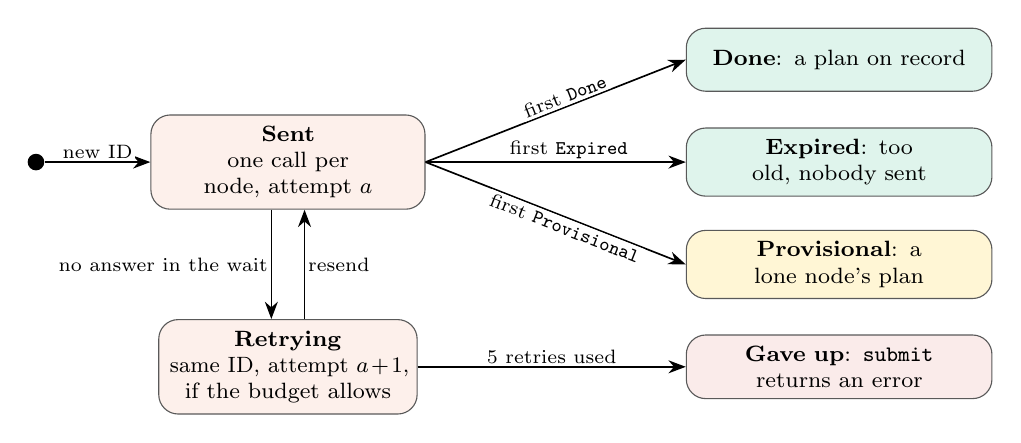
\begin{tikzpicture}[x=1cm,y=1cm]
  \node[sinit] (i) at (0,0) {};
  \node[state, fill=clientorange!10, text width=3.2cm] (sent) at (3.2,0) {\textbf{Sent}\\ one call per node, attempt $a$};
  \node[state, fill=clientorange!10, text width=3.0cm] (retry) at (3.2,-2.6) {\textbf{Retrying}\\ same ID, attempt $a+1$, if the budget allows};
  \node[state, fill=mwgreen!14, text width=3.6cm] (done) at (10.2,1.3) {\textbf{Done}: a plan on record};
  \node[state, fill=mwgreen!14, text width=3.6cm] (exp) at (10.2,0) {\textbf{Expired}: too old, nobody sent};
  \node[state, fill=notefill, text width=3.6cm] (prov) at (10.2,-1.3) {\textbf{Provisional}: a lone node's plan};
  \node[state, fill=badred!10, text width=3.6cm] (gave) at (10.2,-2.6) {\textbf{Gave up}: \code{submit} returns an error};
  \draw[flow] (i) -- node[elabel, above]{new ID} (sent);
  \draw[flow] (sent.east) -- node[elabel, above, sloped, pos=0.55]{first \code{Done}} (done.west);
  \draw[flow] (sent.east) -- node[elabel, above, pos=0.55]{first \code{Expired}} (exp.west);
  \draw[flow] (sent.east) -- node[elabel, below, sloped, pos=0.55]{first \code{Provisional}} (prov.west);
  \draw[flow] ([xshift=-6pt]sent.south) -- node[elabel, left]{no answer in the wait} ([xshift=-6pt]retry.north);
  \draw[flow] ([xshift=6pt]retry.north) -- node[elabel, right]{resend} ([xshift=6pt]sent.south);
  \draw[flow] (retry) -- node[elabel, above]{5 retries used} (gave);
\end{tikzpicture}
\caption{One report as the client middleware sees it. On any answer the client cancels its calls still open on the other nodes. An answer to an earlier attempt still counts.}
\label{fig:client-states}
\end{figure}

\subsection{Choice of RPC}
\label{sec:rpc}

The class notes of Oct 4 ask us not to go down to raw UDP but to use a ready-made RPC or RMI system and say why, and the notes of Oct 28 point at the table in Chapter 2 of Java RMI, CORBA and Sun RPC. We chose RPC, not RMI, and the library \texttt{tarpc} \cite{tarpc} as the system (\dlog{D119}, \dlog{D176}). Our service is procedures over replicated state: nothing in it has an object identity that a client would name or hold, which is what RMI adds. Rust rules out using Java RMI or CORBA as they are, so we compared tarpc with them on the same rows (Table~\ref{tab:rpc}).

\begin{table}[!htb]
\centering\small
\caption{tarpc against the systems in the slides (\dlog{D176}).}
\label{tab:rpc}
\begin{tabularx}{\linewidth}{@{}P{2.6cm}LLLL@{}}
\toprule
 & Java RMI & CORBA & Sun RPC & tarpc (ours) \\
\midrule
Style & RMI & RMI & RPC & RPC \\
Languages & Java only & many & many & Rust only \\
Interface & remote interface & CORBA IDL & Sun XDR & a Rust trait with \texttt{\#[tarpc::service]} \\
Marshalling & Java serialization & CDR & XDR & serde with bincode \\
Semantics alone & at-most-once & at-most-once & at-least-once & maybe: it never resends \\
\bottomrule
\end{tabularx}
\end{table}

tarpc on its own gives ``maybe'' semantics, so at-most-once is our work (\dlog{D177}). From client to cloud, the effect of a report is recorded at most once across all replicas: the client resends with the same ID, the results table filters duplicates by ID, and any node re-sends the answer from its copy. Peer calls are ``maybe'': a lost bid or heartbeat is simply covered by the next one. The one labelled exception is a provisional answer from a node alone, which can differ from what is recorded later (Section~\ref{sec:degraded}).

\textbf{Why UDP for reports.} The note ``Request reply protocol + UDP'' can be read as ``use UDP'' or as ``UDP is the level not to go down to''. We did both: reports travel over UDP, but our UDP adapter holds no RPC logic. Call IDs, deadlines and matching replies to calls stay tarpc's, and retries stay in the middleware (\dlog{D178}). UDP saves the connection set-up per client and node, the pings and reconnects, and acknowledgements that a reply already gives. It costs a full wait when an answer is lost, a larger kernel buffer and a firewall rule.

% ==============================================================================================
\section{The elections}
\label{sec:election}

\subsection{What the survey found}

In Phase 0 each team member surveyed one election algorithm, and the team compared them on the same rows \cite{survey}. Table~\ref{tab:survey} is a short form of that comparison. Three findings shaped everything after it. First, with only three peers, message complexity does not matter: even the $O(n^2)$ algorithms need only a few messages. Second, the assumptions about failure matter most. The ring algorithms assume no node fails during an election, and in RescueMesh an election happens because a node failed. Bully depends on a timeout that tells a slow node from a dead one, which no timeout can do \cite{chandra}, so it can end with two coordinators. Third, electing a coordinator and choosing a node for each request are two different jobs. A coordinator stays until it fails, while load changes with every request.

\begin{table}[!htb]
\centering\scriptsize
\caption{The surveyed algorithms, in short \cite{survey}. $n$ is the number of nodes; RescueMesh has 3.}
\label{tab:survey}
\begin{tabularx}{\linewidth}{@{}P{1.9cm}LLLp{1.3cm}L@{}}
\toprule
 & Assumes & Messages & Failures & Uses load & Fit for RescueMesh \\
\midrule
Bully \cite{garcia} & bounded delay, reliable delivery & $n-2$ best, $O(n^2)$ worst & tolerated by timeouts & no & a silent node that returns can make two coordinators \\
Chang-Roberts & a ring, no failures in an election & $3n-1$ worst for one starter & none & no & only with failure detection and ring repair added \\
Hirschberg-Sinclair & a two-way ring, no failures & $O(n \log n)$ & none & no & its advantage needs a large ring \\
Raft \cite{raft} & a majority up, stable storage & $O(n)$ per election, plus heartbeats & new election while a majority lives & no & fits coordinator, replication and recovery \\
ZooKeeper FLE & a quorum & $O(n^2)$ per round & new election while a quorum lives & no & elects only; replication is elsewhere \\
Load bidding \cite{contractnet} & unique request IDs, a bid timeout & $n$ to $n(n-1)$ per request & next bidder takes over & yes & fits the choice of node per request \\
\bottomrule
\end{tabularx}
\end{table}

\textbf{The survey's choice.} Two mechanisms, one per job: Raft leader election for the cloud coordinator, and a load-based bidding election for the node that plans each report, which the survey called ``Bully adapted to load'', since a node's priority is its load and not its ID. The survey also gave the Raft leader the fault injection and the recovery of a returning node. Table~\ref{tab:jobs} shows how each of these choices ended up. Section~\ref{sec:raft} tells the story of the first row.

\begin{table}[!htb]
\centering\small
\caption{The election jobs: what the survey chose and what was built.}
\label{tab:jobs}
\begin{tabularx}{\linewidth}{@{}P{3.0cm}LL@{}}
\toprule
Job & Chosen in the survey (Oct 4) & Built in the final system \\
\midrule
Order of the shared log & Raft leader election & No leader: every node sorts the same batches \\
Node that plans a report & Load bidding & Load bidding, as chosen \\
Node that fails next & chosen by the Raft leader & a draw by all three nodes \\
Recovery of a returning node & the Raft leader sends what it missed & any member sends what it missed \\
\bottomrule
\end{tabularx}
\end{table}

\subsection{The bidding election, for every report}
\label{sec:bidding}

Every node that receives a report and is serving opens a round for it, sends its bid to its peers, and waits 60 ms from when the report reached it. Then it closes the round by itself. The lowest bid wins, ties go to the lower node ID, and the order of the bids is also the takeover order. There is no ``you won'' message. Every node works out the same winner from the same bids, so nobody coordinates. This follows the announce, bid and award shape of the contract net protocol \cite{contractnet}, except that every node does the award by itself. Each attempt of a report has its own round, so a retry bids again with fresh load.

\textbf{The bid} is the expected wait at this node, in microseconds:
\[
\mathit{score} = \frac{(\mathit{queued} + \mathit{running} + \mathit{won} + 1) \times \mathit{service}}{\mathit{workers}}
\]
Here \emph{queued} and \emph{running} are the worker pool's jobs, \emph{won} counts rounds this node won or is leading but has not started yet, and \emph{service} is a running average of its own planning time in microseconds. The $+1$ counts the report being bid on, so an idle fast node beats an idle slow one. \emph{won} matters because a node can win many rounds before its queue shows them; without it, every report in a burst would go to the same node, which the survey warned of \cite{survey}. In the report traced in Figure~\ref{fig:seq-report}, node 3 had 123 such rounds and a planning time of 8 $\mu$s with 20 workers, so it bid $(123+1) \times 8 / 20 = 49$.

Expected wait was chosen over the other variants because it measured best. Scenario 2 in Section~\ref{sec:lb} compares it with a queue-only score: when one node's planning was made 5 times slower, the queue-only score barely changed its bid, because a slow plan does not show in the queue at that load, while expected wait moved most of the work away.

\textbf{When bids are missed.} A node that misses a bid can decide differently from the others. Then two nodes both plan a report, or none does until the backstop. This costs work and time and is never wrong, because the first result recorded wins. At high load fewer rounds see all three bids, which is what limits fairness above 30,000 reports a second (Table~\ref{tab:elcost}).

\begin{table}[!htb]
\centering\small
\caption{What the bidding election costs, on the overnight build, 5 runs per row. ``All 3 bids'' is the share of rounds that saw every node's bid. Calls are per request; bids are sent in groups, so there are far fewer calls than bids.}
\label{tab:elcost}
\begin{tabular}{@{}rrrrrrr@{}}
\toprule
Offered/s & Planning work & Election p50 ms & p99 ms & All 3 bids & Bid calls & Fairness (Jain) \\
\midrule
5,000 & 0 & 61.0 & 62.0 & 97.7\% & 0.089 & 0.999 \\
10,000 & 0 & 61.0 & 62.0 & 96.2\% & 0.044 & 0.997 \\
20,000 & 0 & 61.1 & 62.4 & 92.3\% & 0.022 & 0.999 \\
30,000 & 0 & 61.2 & 65.1 & 73.7\% & 0.014 & 0.998 \\
35,000 & 0 & 61.4 & 72.5 & 32.5\% & 0.009 & 0.900 \\
1,000 & 1000 & 61.0 & 61.9 & 99.0\% & 0.426 & 1.000 \\
10,000 & 1000 & 61.0 & 62.0 & 96.6\% & 0.044 & 0.998 \\
12,000 & 1000 & 61.0 & 62.2 & 95.5\% & 0.037 & 0.998 \\
14,000 & 1000 & 61.0 & 62.6 & 88.6\% & 0.033 & 1.000 \\
\bottomrule
\end{tabular}
\end{table}

An election takes its 60 ms window plus scheduling. The window is a setting: a smaller one answers faster but sees fewer bids, so more reports get planned twice. Fairness is Jain's index over the three nodes' shares \cite{jain}: 1 means perfectly even.

\subsection{Takeover: when the winner goes quiet}
\label{sec:takeover}

Every node that lost a round stands by. If the winner is suspected, or nothing for that report is recorded within the backstop of at least 1.5 s, the next node in the round's ranking plans it. If the old winner's result arrives later, it is a duplicate and changes nothing. Figure~\ref{fig:seq-takeover} shows the case.

\begin{figure}[!htb]
\centering
\resizebox{\linewidth}{!}{%
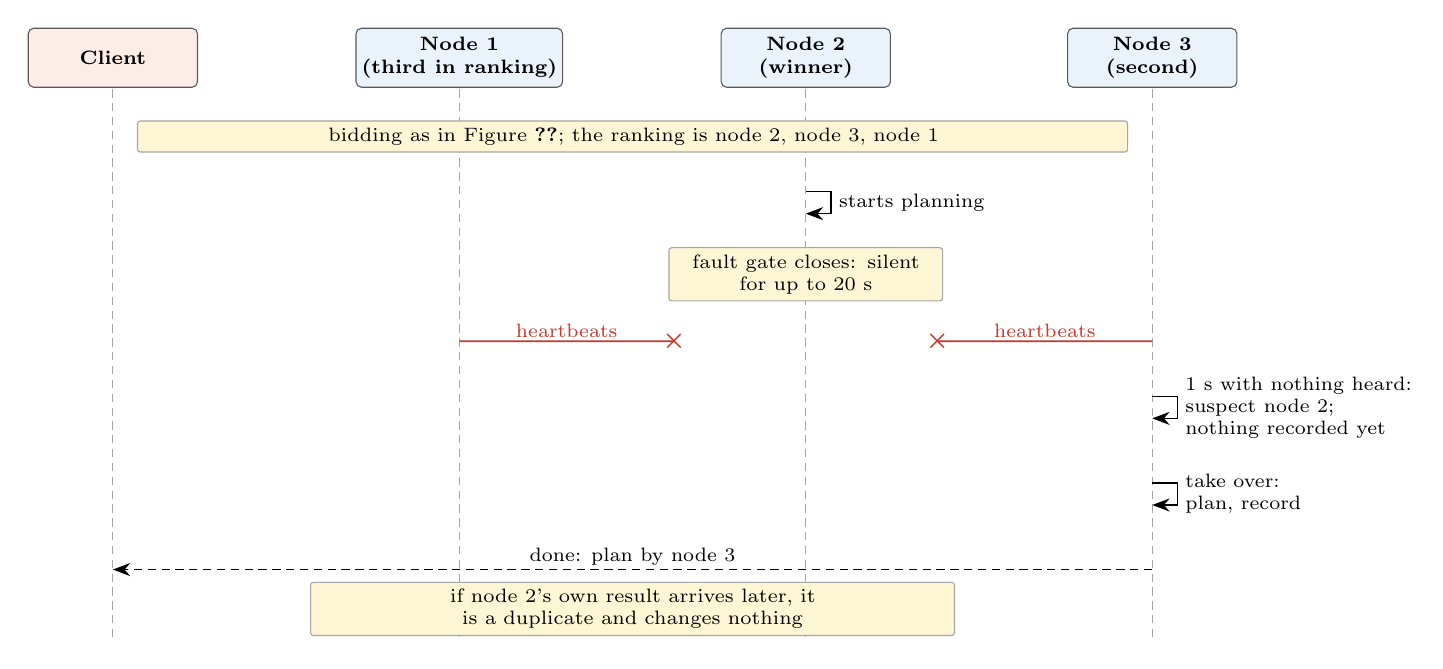
\begin{tikzpicture}[x=1cm,y=1cm]
  \seqactor[clientorange!12]{0}{Client}{-7.4}
  \seqactor{4.4}{Node 1\\(third in ranking)}{-7.4}
  \seqactor{8.8}{Node 2\\(winner)}{-7.4}
  \seqactor{13.2}{Node 3\\(second)}{-7.4}
  \seqnote{6.6}{-1.0}{12.4}{bidding as in Figure~\ref{fig:seq-report}; the ranking is node 2, node 3, node 1}
  \seqself{8.8}{-1.7}{starts planning}
  \seqnote{8.8}{-2.75}{3.3}{fault gate closes: silent\\ for up to 20 s}
  \seqlost{13.2}{8.8}{-3.6}{heartbeats}
  \seqlost{4.4}{8.8}{-3.6}{heartbeats}
  \seqself{13.2}{-4.3}{1 s with nothing heard:\\ suspect node 2;\\ nothing recorded yet}
  \seqself{13.2}{-5.4}{take over:\\ plan, record}
  \seqrep{13.2}{0}{-6.5}{done: plan by node 3}
  \seqnote{6.6}{-7.0}{8.0}{if node 2's own result arrives later, it is a duplicate and changes nothing}
\end{tikzpicture}}
\caption{Takeover. Node 1 also stands by; it would plan only if node 3 were also silent. The same happens without a fault if the winner is merely slow, at the 1.5 s backstop.}
\label{fig:seq-takeover}
\end{figure}

\subsection{The fault election}
\label{sec:faultelection}

The spec requires the three cloud servers to elect, from time to time, one machine to ignore communication for up to 20 s. The survey had the Raft leader choose. This was changed so that no node decides for another: every 30 to 60 s, the three nodes draw random numbers and send them to each other, and the highest goes silent for its own drawn time of 1 to 20 s. The first node whose timer runs out starts a round, and the others draw as soon as they hear of it, so starting a round gives no power. A node that is missing any of the three numbers does nothing, so a node that is off, silent or catching up blocks the next fault. That keeps faults to one at a time on this path. Figure~\ref{fig:seq-faultel} shows a round.

\begin{figure}[!htb]
\centering
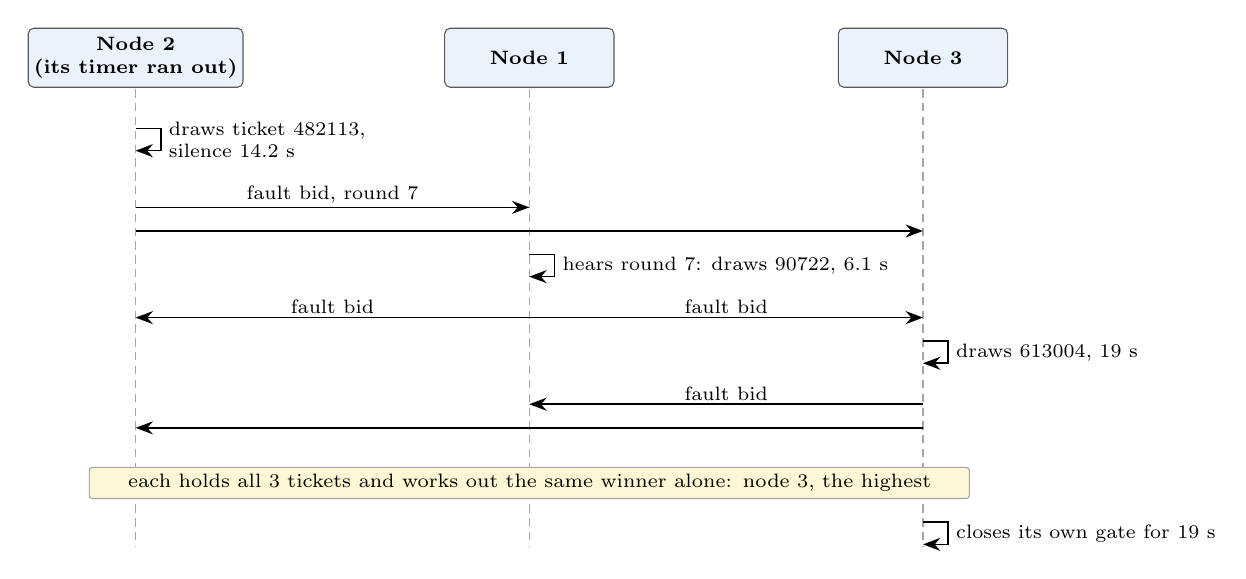
\begin{tikzpicture}[x=1cm,y=1cm]
  \seqactor{0}{Node 2\\(its timer ran out)}{-6.2}
  \seqactor{5.0}{Node 1}{-6.2}
  \seqactor{10.0}{Node 3}{-6.2}
  \seqself{0}{-0.9}{draws ticket 482113,\\ silence 14.2 s}
  \seqmsg{0}{5.0}{-1.9}{fault bid, round 7}
  \seqmsg{0}{10.0}{-2.2}{}
  \seqself{5.0}{-2.5}{hears round 7: draws 90722, 6.1 s}
  \seqmsg{5.0}{0}{-3.3}{fault bid}
  \seqmsg{5.0}{10.0}{-3.3}{fault bid}
  \seqself{10.0}{-3.6}{draws 613004, 19 s}
  \seqmsg{10.0}{5.0}{-4.4}{fault bid}
  \seqmsg{10.0}{0}{-4.7}{}
  \seqnote{5.0}{-5.4}{11.0}{each holds all 3 tickets and works out the same winner alone: node 3, the highest}
  \seqself{10.0}{-5.9}{closes its own gate for 19 s}
\end{tikzpicture}
\caption{One round of the fault election. The others suspect node 3 about 1 s later and go on without it. Nothing goes through the shared log, and no node is in charge.}
\label{fig:seq-faultel}
\end{figure}

In the experiments the fault election was measured on its own, in 5 runs of 5 minutes at 3,000 reports a second with faults every 20 to 30 s: 47 elected faults, every node elected at least once in 4 of the 5 runs, nobody gave up, and the others dropped the silent node in a median of 1,018 ms (Section~\ref{sec:s4}). In the other experiment cells, the script silences the node at a fixed time with the operator tool, so that runs can be compared.

% ==============================================================================================
\section{Raft: why it was chosen, why it was replaced, and the measurements}
\label{sec:raft}

The biggest decision that changed in this phase was the shared log. The system started with Raft, as the survey recommended, was built on it, and was measured on the six PCs. On November 4, Raft was replaced with the team's own shared log, which has no leader (\dlog{D249}). This section explains the choice, the problems that led to the change, and the results on both sides. Figure~\ref{fig:timeline} gives the order of events.

\begin{figure}[!htb]
\centering
\resizebox{\linewidth}{!}{%
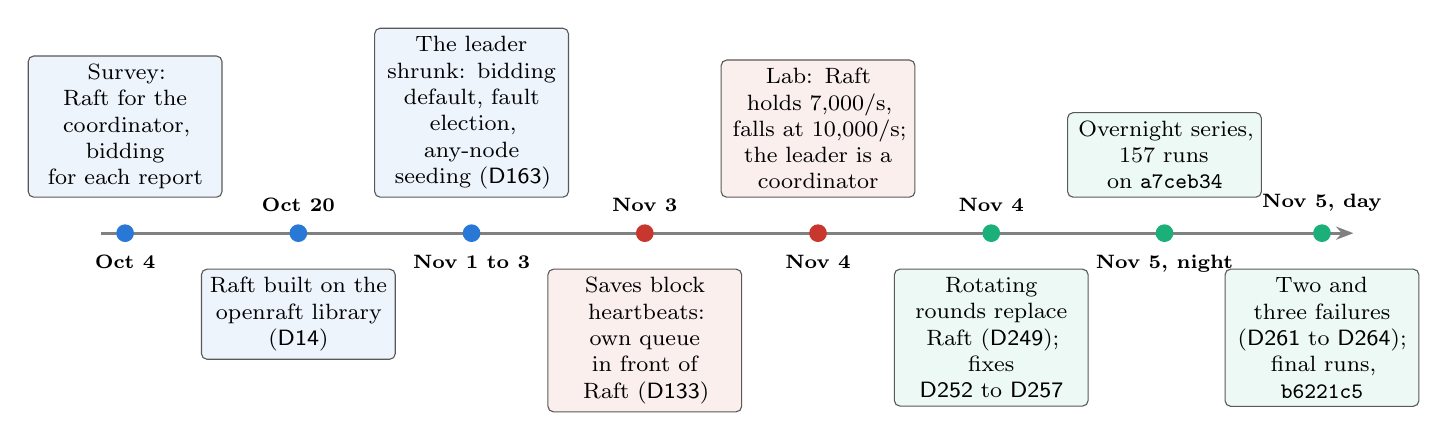
\begin{tikzpicture}[x=1cm,y=1cm, every node/.style={font=\scriptsize}]
  \draw[very thick, black!50, ->] (-0.3,0) -- (15.6,0);
  \foreach \x/\d/\t/\c/\side in {
      0.0/Oct 4/{Survey: Raft for the\\ coordinator, bidding\\ for each report}/nodeblue/1,
      2.2/Oct 20/{Raft built on the\\ openraft library\\ (\dlog{D14})}/nodeblue/-1,
      4.4/Nov 1 to 3/{The leader shrunk: bidding\\ default, fault election,\\ any-node seeding (\dlog{D163})}/nodeblue/1,
      6.6/Nov 3/{Saves block heartbeats:\\ own queue in front of\\ Raft (\dlog{D133})}/badred/-1,
      8.8/Nov 4/{Lab: Raft holds 7,000/s,\\ falls at 10,000/s;\\ the leader is a\\ coordinator}/badred/1,
      11.0/Nov 4/{Rotating rounds replace\\ Raft (\dlog{D249}); fixes\\ \dlog{D252} to \dlog{D257}}/mwgreen/-1,
      13.2/{Nov 5, night}/{Overnight series,\\ 157 runs on \commit{a7ceb34}}/mwgreen/1,
      15.2/{Nov 5, day}/{Two and three failures\\ (\dlog{D261} to \dlog{D264});\\ final runs, \commit{b6221c5}}/mwgreen/-1} {
    \fill[\c] (\x,0) circle (3.2pt);
    \node[font=\scriptsize\bfseries, anchor=\ifnum\side>0 north\else south\fi] at (\x,{-0.15*\side}) {\d};
    \node[box, fill=\c!8, text width=2.25cm, anchor=\ifnum\side>0 south\else north\fi] at (\x,{0.45*\side}) {\t};
  }
\end{tikzpicture}}
\caption{How the shared log changed during Phase 1. Blue is the Raft design, red the problems the lab found, green the design with no leader.}
\label{fig:timeline}
\end{figure}

\subsection{Why Raft was chosen}

The survey compared six algorithms and chose Raft to elect the cloud's coordinator (\dlog{D1}) \cite{survey}. The reasons still hold as reasons, and they are stated fairly here:

\begin{itemize}
  \item \textbf{Safety without trusting timeouts.} Raft elects at most one leader per term by majority vote, and a committed entry is never lost, however late messages are \cite{raft}. Timeouts affect only how fast it reacts. Bully, by contrast, can end with two coordinators when a slow node is taken for a dead one.
  \item \textbf{Three nodes survive one failure.} A majority of three is two, so the cloud keeps going while one node is silent, which is exactly the spec's fault.
  \item \textbf{One protocol for election and replication.} Raft's log gives every node the same incidents, responders and results, and a returning node gets what it missed from the leader. No second mechanism was needed for the state.
  \item \textbf{A tested library.} The team used openraft 0.9.25 \cite{openraft} rather than writing Raft from scratch, which would have taken weeks before anything could be tested (\dlog{D4}, \dlog{D14}).
\end{itemize}

The survey was clear that Raft does not choose a node by load, so the bidding election stayed separate. It also listed Raft's costs: more machinery than Bully or a ring, a gap with no leader after a failure, and ``all write requests go through the leader, so the leader can become a bottleneck'' \cite{survey}. That last line turned out to matter most.

\subsection{What the Raft design looked like}

Figure~\ref{fig:seq-raft} shows one report in the Raft design. The bidding already chose the node that plans, so the leader planned nothing unless it won a bid. But every result went to the leader, which put it in the log, copied it to the followers, and counted it as committed once two of three nodes had saved it.

\begin{figure}[!htb]
\centering
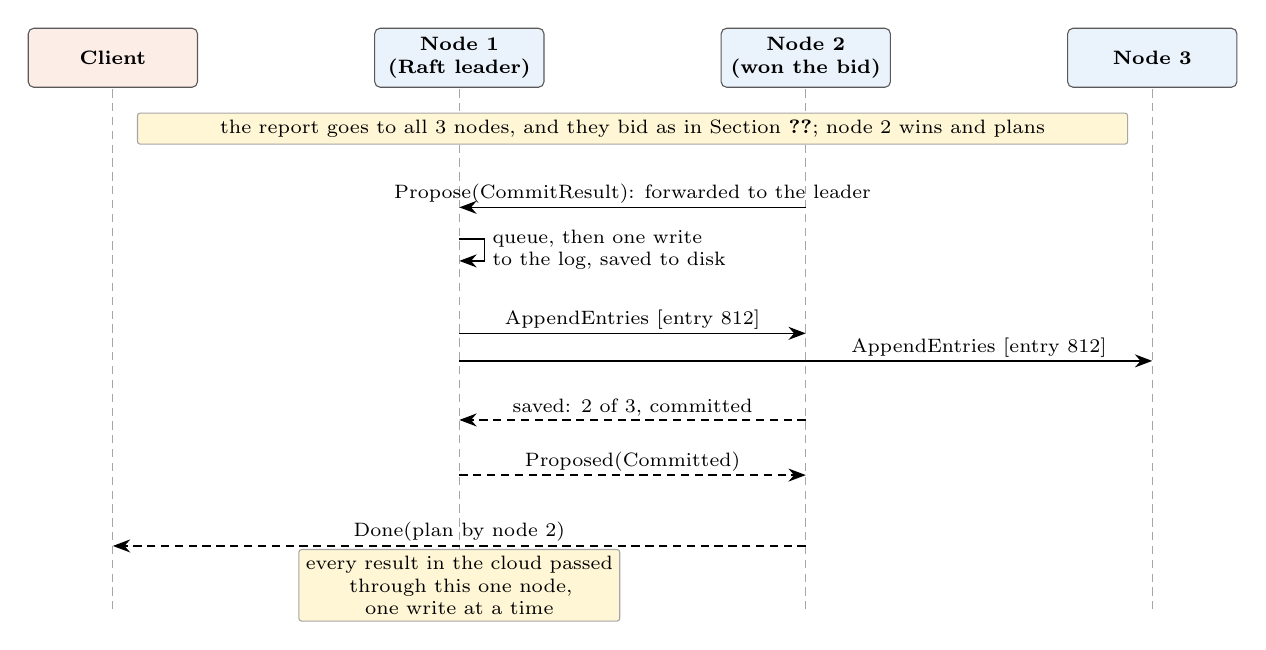
\begin{tikzpicture}[x=1cm,y=1cm]
  \seqactor[clientorange!12]{0}{Client}{-7.0}
  \seqactor{4.4}{Node 1\\(Raft leader)}{-7.0}
  \seqactor{8.8}{Node 2\\(won the bid)}{-7.0}
  \seqactor{13.2}{Node 3}{-7.0}
  \seqnote{6.6}{-0.9}{12.4}{the report goes to all 3 nodes, and they bid as in Section~\ref{sec:bidding}; node 2 wins and plans}
  \seqmsg{8.8}{4.4}{-1.9}{Propose(CommitResult): forwarded to the leader}
  \seqself{4.4}{-2.3}{queue, then one write\\ to the log, saved to disk}
  \seqmsg{4.4}{8.8}{-3.5}{AppendEntries [entry 812]}
  \seqmsg{4.4}{13.2}{-3.85}{}
  \node[mlabel] at (11.0,-3.85) {AppendEntries [entry 812]};
  \seqrep{8.8}{4.4}{-4.6}{saved: 2 of 3, committed}
  \seqrep{4.4}{8.8}{-5.3}{Proposed(Committed)}
  \seqrep{8.8}{0}{-6.2}{Done(plan by node 2)}
  \seqnote{4.4}{-6.7}{3.9}{every result in the cloud passed\\ through this one node, one write at a time}
\end{tikzpicture}
\caption{One report under Raft (before \dlog{D249}). The leader decides nothing about the plan, but it orders every result, sends every copy, and its write path is shared by all reports.}
\label{fig:seq-raft}
\end{figure}

\subsection{What went wrong}
\label{sec:raftproblems}

Five problems came up: one against the project's requirements, and four in rehearsals on one PC and then on the six lab PCs. Table~\ref{tab:raftproblems} lists them with the evidence for each.

\begin{table}[!htb]
\centering\small
\caption{The shortcomings of the Raft design, and the evidence for each.}
\label{tab:raftproblems}
\begin{tabularx}{\linewidth}{@{}P{3.2cm}LL@{}}
\toprule
Problem & Evidence & What was tried before switching \\
\midrule
1. The leader is a coordinator & The project requires the leader of an election not to act as a coordinator, and the nodes to be peers \cite{notes}. In Raft every commit passes through the leader. & Every decision was moved away from the leader: bidding picks the planner (\dlog{D114}), the fault election picks the victim (\dlog{D158}), any node loads the responders (\dlog{D164}). The leader only ordered the log (\dlog{D163}). A strict reader could still call that a coordinator, and the design log said so. \\
2. Disk saves silenced the leader & openraft saves each log entry inside its core task, and can work through up to 1,000 queued writes before it sends a heartbeat. In a one-PC rehearsal with 300 users, the followers stopped hearing the leader 0.78 s into the load: 225 elections in one run, and not one report answered (\dlog{D133}). & A queue of the team's own in front of openraft: one write in flight per node, and everything waiting goes into that one write. It fixed the elections, at the cost of a second queue to tune. \\
3. One write at a time through one node & At \commit{0397d37}, the leader sent one write at a time of at most 200 commands. Measured: about 46 ms per write between PCs, so a ceiling of about 4,350 commands, or 1,630 reports, a second. On one PC over loopback the same write took 4.3 ms. & Bigger writes (\dlog{D234}), grouped bids and forwards (\dlog{D247}, \dlog{D248}). The ceiling rose, but stayed at the leader. \\
4. Overload fed itself & When commits slowed, losers of a bid took over the report, plans went stale, clients retried and elections followed. Figure~\ref{fig:collapse}(a) shows it second by second. & Longer backstop (\dlog{D235}), fewer scans of the responder table (\dlog{D238} to \dlog{D246}). \\
5. A busy leader cannot hand over & A busy leader slows every commit, but openraft 0.9.25 has no command to hand leadership over, and followers refuse votes while the leader's lease holds (\dlog{D217}, \dlog{D218}). & A busy leader stops its own heartbeats so that a normal vote picks another. Each change costs about 0.8 s with no answers. \\
\bottomrule
\end{tabularx}
\end{table}

Problems 3 and 4 together set the throughput limit. Figure~\ref{fig:collapse}(a) is from a run on the six PCs at only 800 reports a second, summed over the nodes. A commit took about 85 ms when healthy. Then one peer went quiet for 157 ms, commits slowed past the takeover backstop, nodes that had lost the bid started planning the same reports, and the extra plans slowed commits further. Clients retried after 2 s, so a node that normally received about 2,400 requests a second soon received over 5,000. Elections came last, as a result. In another run at 1,000 a second, the Raft term stayed at 3 for 45 s and then rose to about 90.

\begin{figure}[!htb]
\centering
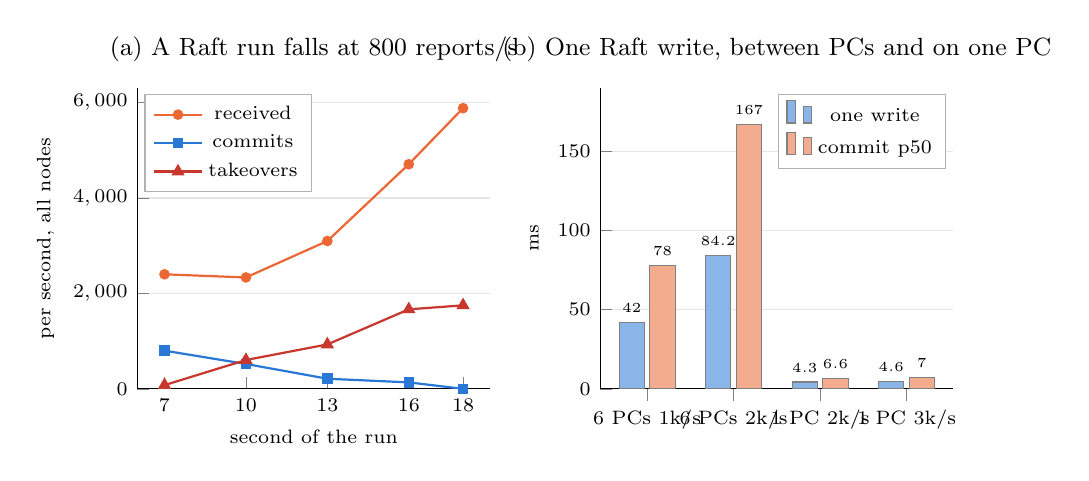
\begin{tikzpicture}
\begin{axis}[
  name=a, width=0.5\linewidth, height=5.4cm,
  xlabel={second of the run}, ylabel={per second, all nodes},
  xmin=6, xmax=19, ymin=0, ymax=6300, xtick={7,10,13,16,18},
  yticklabel style={/pgf/number format/fixed, /pgf/number format/1000 sep={,}, font=\scriptsize},
  xticklabel style={font=\scriptsize}, label style={font=\scriptsize},
  legend style={font=\scriptsize, at={(0.02,0.98)}, anchor=north west, draw=black!30},
  axis lines*=left, ymajorgrids, grid style={black!10},
  title={(a) A Raft run falls at 800 reports/s}, title style={font=\small},
]
\addplot[thick, clientorange, mark=*, mark size=1.5pt] coordinates {(7,2400) (10,2334) (13,3098) (16,4707) (18,5882)};
\addlegendentry{received}
\addplot[thick, nodeblue, mark=square*, mark size=1.5pt] coordinates {(7,800) (10,521) (13,212) (16,135) (18,0)};
\addlegendentry{commits}
\addplot[thick, badred, mark=triangle*, mark size=2pt] coordinates {(7,78) (10,604) (13,931) (16,1666) (18,1750)};
\addlegendentry{takeovers}
\end{axis}
\begin{axis}[
  at={(a.east)}, anchor=west, xshift=1.4cm,
  ybar, bar width=0.32cm, width=0.5\linewidth, height=5.4cm,
  ymin=0, ymax=190, ylabel={ms},
  symbolic x coords={6 PCs 1k/s, 6 PCs 2k/s, 1 PC 2k/s, 1 PC 3k/s}, xtick=data,
  xticklabel style={font=\scriptsize, align=center}, yticklabel style={font=\scriptsize}, label style={font=\scriptsize},
  legend style={font=\scriptsize, at={(0.98,0.98)}, anchor=north east, draw=black!30},
  nodes near coords, nodes near coords style={font=\tiny},
  axis lines*=left, ymajorgrids, grid style={black!10}, enlarge x limits=0.18,
  title={(b) One Raft write, between PCs and on one PC}, title style={font=\small},
]
\addplot[fill=nodeblue!55, draw=black!50] coordinates {(6 PCs 1k/s,42.0) (6 PCs 2k/s,84.2) (1 PC 2k/s,4.3) (1 PC 3k/s,4.6)};
\addlegendentry{one write}
\addplot[fill=clientorange!55, draw=black!50] coordinates {(6 PCs 1k/s,78) (6 PCs 2k/s,167) (1 PC 2k/s,6.6) (1 PC 3k/s,7.0)};
\addlegendentry{commit p50}
\end{axis}
\end{tikzpicture}
\caption{Why Raft was slow on the lab PCs. (a) Second by second, in \texttt{rate-800b} at \commit{0397d37} with \texttt{plan\_work} 1000: received means requests reaching the nodes, so it includes retries; from second 18 commits are about 0. (b) Same build and settings (\commit{4d67039}), seconds 5 to 25 of each run: one write through the leader took 10 to 20 times longer between PCs than on one PC, while a disk sync took 3.2 to 4.2 ms against 2.2 to 2.3 ms. The time was in the path between PCs, not in the disk.}
\label{fig:collapse}
\end{figure}

\textbf{Why the switch.} Problem 1 could not be fixed while Raft stayed: as long as one elected node orders every commit, the cloud has a coordinator, and the requirement is a cloud of peers with none. On the same day, the best Raft build held 7,000 reports a second and fell at 10,000 (\dlog{D249}), while the target for the system was at least 10,000. The step that held throughput back was the one-at-a-time path through the leader, so a leaderless log could remove both problems at once. Three options were considered (\dlog{D249}). Each node owning a share of the responders with no global order would have changed the state, the digests, recovery and the analysis, and a lost node would take a third of the responders with it. Deleting Raft outright would have rewritten about 15 test files with no way back. The team chose rotating rounds behind the same \code{Consensus} interface (Section~\ref{sec:consensus-trait}), so that nothing above the log changed and Raft stayed available as a setting. The team also looked for a library that orders a log with no leader, and tested the closest one on the three node PCs; it failed when one node stopped (\dlog{D259}, Section~\ref{sec:library}).

\subsection{Results with Raft}

\textbf{The 21-cell plan.} The first full experiment plan ran on Raft, at \commit{0397d37}, with 3 runs per cell and closed-loop users: 1,372,598 operations in all. Table~\ref{tab:raftplan} shows the main cells. Every cell had 0 digest mismatches and 0 reports unaccounted for, so Raft kept the state correct throughout. These runs had a bug that was found later: the campus generator tied zone and capability together, so only half of the zone and capability pairs had responders (\dlog{D240}).

\begin{table}[!htb]
\centering\small
\caption{The Raft plan at \commit{0397d37}: mean of 3 runs, closed-loop users, \texttt{plan\_work} 1000. ``Leader'' cells use leader dispatch, the baseline in which the Raft leader plans every report. The gap is the longest time a client PC had no answer, in the worst run.}
\label{tab:raftplan}
\begin{tabular}{@{}lrrrrrrr@{}}
\toprule
Cell & Answered/s & p50 ms & p99 ms & Gave up & Retried & Gap ms & Elections \\
\midrule
300 users, bidding & 268.1 & 95.3 & 349.8 & 0 & 0\% & 213 & 0 \\
300 users, leader & 285.0 & 42.4 & 181.7 & 0 & 0\% & 227 & 0 \\
1,000 users, bidding & 870.1 & 126.5 & 390.9 & 0 & 0.0\% & 274 & 0 \\
1,000 users, leader & 934.6 & 60.2 & 181.5 & 0 & 0.2\% & 168 & 0 \\
3,000 users, bidding & 286.8 & 6,600 & 26,006 & 304.7 & 98.8\% & 551 & 0 \\
3,000 users, leader & 1,059.7 & 135.9 & 16,245 & 92.7 & 41.4\% & 256 & 0 \\
300 users, leader silenced & 268.3 & 89.8 & 515.6 & 0 & 0.1\% & 969 & 1 \\
1,500 users, leader silenced & 614.2 & 492.7 & 7,062 & 0 & 30.0\% & 1,445 & 1 \\
300 users, two nodes down & 240.9 & 98.2 & 5,742 & 0 & 4.2\% & 3,604 & 55 \\
\bottomrule
\end{tabular}
\end{table}

Three results here are worth saying plainly. First, \textbf{failover under Raft was fast}: a new leader in 802 ms on average at 300 users and 841 ms at 1,500, and nobody gave up. Second, \textbf{on Raft, bidding lost to leader dispatch}. At low load leader dispatch answered in half the time, because bidding waits for its window and then forwards the result to the leader anyway, and at 3,000 users bidding collapsed while leader dispatch held better. With Raft underneath, bidding paid for the election and still queued behind the leader. Third, load was not shared evenly under bidding at 300 users (Jain 0.594, with node 3 winning 72\%). It later turned out that node 3 alone had its CPU energy setting at \texttt{performance}, so its plans took 3.2 ms against 7.7 and 9.4 ms on the others, and bidding correctly sent it more work. That is evidence that the bid follows real speed, but it made the plan's fairness numbers uneven.

Figure~\ref{fig:raft-results} shows two of these results as charts: the median latency of the two policies on Raft, and the p99 latency before, during and after a fault in the lab guide's tests on Raft.

\begin{figure}[!htb]
\centering
\begin{minipage}[b]{0.49\linewidth}
\centering
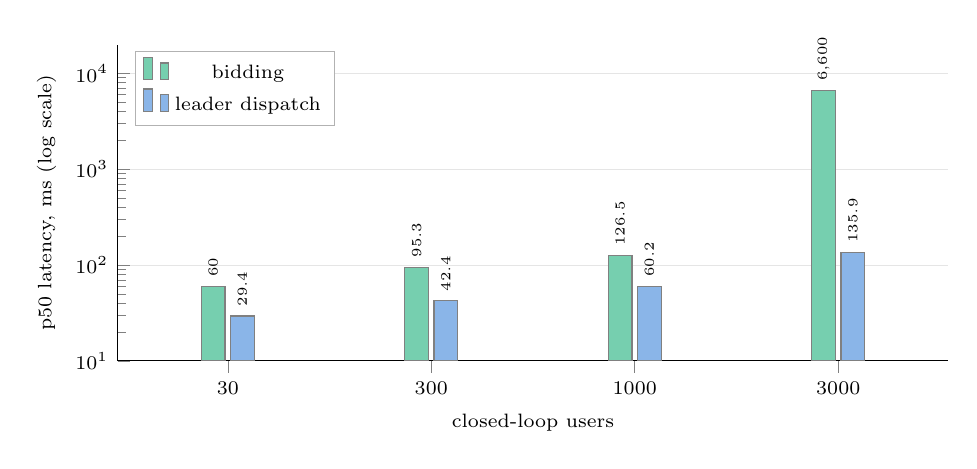
\begin{tikzpicture}
\begin{axis}[
  ybar, bar width=0.3cm, width=\linewidth, height=5.6cm,
  ymode=log, log origin=infty, ymin=10, ymax=20000, ylabel={p50 latency, ms (log scale)},
  symbolic x coords={30, 300, 1000, 3000}, xtick=data, xlabel={closed-loop users},
  xticklabel style={font=\scriptsize}, yticklabel style={font=\scriptsize}, label style={font=\scriptsize},
  legend style={font=\scriptsize, at={(0.02,0.98)}, anchor=north west, draw=black!30},
  nodes near coords, nodes near coords style={font=\tiny, rotate=90, anchor=west},
  point meta=rawy, axis lines*=left, ymajorgrids, grid style={black!10}, enlarge x limits=0.18,
]
\addplot[fill=mwgreen!60, draw=black!50] coordinates {(30,60.0) (300,95.3) (1000,126.5) (3000,6600)};
\addlegendentry{bidding}
\addplot[fill=nodeblue!55, draw=black!50] coordinates {(30,29.4) (300,42.4) (1000,60.2) (3000,135.9)};
\addlegendentry{leader dispatch}
\end{axis}
\end{tikzpicture}
\par\small (a) Bidding against leader dispatch on Raft
\end{minipage}\hfill
\begin{minipage}[b]{0.49\linewidth}
\centering
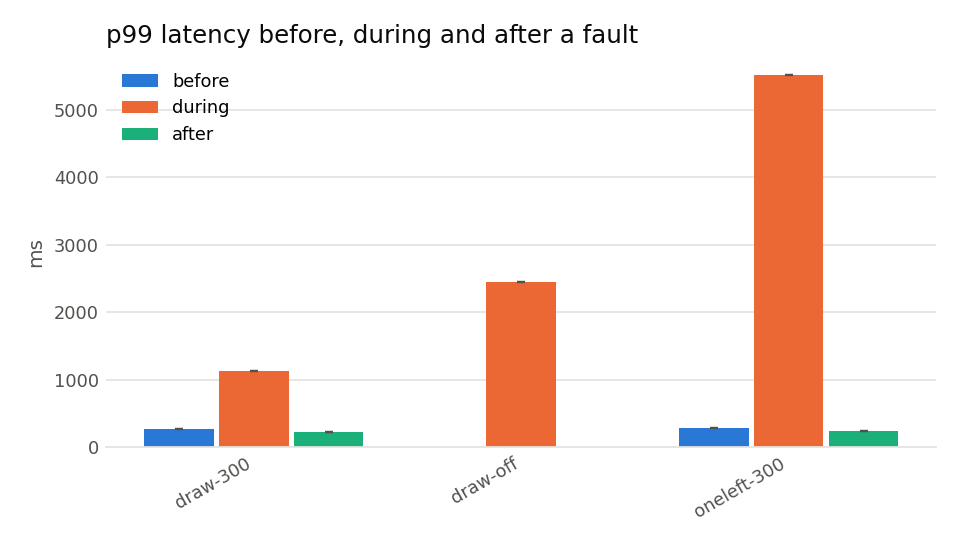
\includegraphics[width=\linewidth]{figures/raft-fault-phases.png}
\par\small (b) p99 around a fault on Raft, from the logs
\end{minipage}
\caption{Results with Raft at \commit{0397d37}. (a) The E1 cells of Table~\ref{tab:raftplan}, mean of 3 runs. (b) The lab guide's T4 with the fault election running (\texttt{draw-300}), T4 with one node off so no draw can go ahead (\texttt{draw-off}, which has no before and after), and T2 with one node killed and one silenced (\texttt{oneleft-300}). Made by \texttt{analysis/analyze.py} from the runs in \texttt{runs/hand/}.}
\label{fig:raft-results}
\end{figure}

\textbf{The throughput ladder.} Table~\ref{tab:ladder} lists the highest fixed rate that held at each build, in the order they were built. Raft rose from 600 to 7,000 reports a second as each limit was fixed, and never reached 10,000.

\begin{table}[!htb]
\centering\small
\caption{Highest offered rate that held, per build, on the six PCs. ``Held'' means every report answered and nobody gave up. One run per step unless stated. The rates with no planning load are not comparable with those with it.}
\label{tab:ladder}
\begin{tabularx}{\linewidth}{@{}P{1.6cm}P{1.6cm}rp{1.7cm}L@{}}
\toprule
Build & Shared log & Held/s & \texttt{plan\_work} & What fell \\
\midrule
\commit{0397d37} & Raft & 600 & 1000 & 800 in 1 of 3 tries and its 5-minute hold; 1,000 in all 4 \\
\commit{4d67039} & Raft & 1,000 & 1000 & 2,000 after about 30 s \\
\commit{0790478} & Raft & 3,000 & 1000 & 5,000 froze, a bug in that build, fixed at \commit{d544a35} \\
\commit{0c9e8fb} & Raft & 7,000 & see note & 10,000: 2,717 answered a second (\dlog{D249}) \\
\commit{cdec322} & rounds & 25,000 & 0 & 30,000: 3,573 gave up (60,000 responders, 3 s detection) \\
\commit{eba4d14} & rounds & 33,000 & 0 & 34,000 started to break; 30,000 held for 5 minutes \\
\commit{eba4d14} & rounds & 10,000 & 1000 & 15,000: all 20 planning threads busy \\
\commit{a7ceb34} & rounds & 30,000 & 0 & held in 5 of 5 runs; 33,000 and 35,000 in 3 of 5 \\
\commit{a7ceb34} & rounds & 12,000 & 1000 & held in 5 of 5 runs; 14,000 in 0 of 5 \\
\bottomrule
\end{tabularx}
\end{table}

The 7,000 row has a caveat: its answers all came, with nobody giving up, but its p99 was 1.2 s, which failed the stricter test used at the time. The folder's run files record its \texttt{plan\_work}, and that value is not copied into the repository.
% CHECK: confirm the plan_work of the f4 runs (analysis/results/f4-stress-summary.txt) from their run.json on client PC 1.

\textbf{The cleanest comparison.} After the switch, Raft was run once more, on the final code, at 10,000 reports a second with 60,000 responders, by setting \texttt{consensus = "raft"} (\texttt{runs/phase1/raft0/10000}). Nothing else changed. Figure~\ref{fig:raft-vs-rounds} sets it beside the same rate on rotating rounds. Raft is one run and rounds five, so the comparison is indicative, but the gap is not small.

\begin{figure}[!htb]
\centering
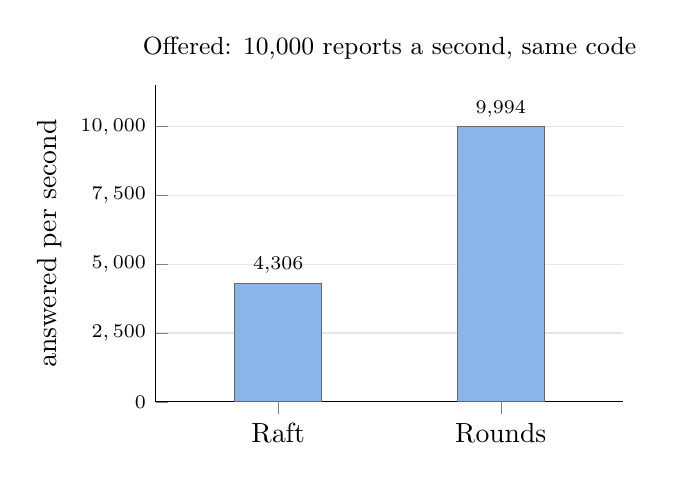
\begin{tikzpicture}
\begin{axis}[
  ybar, bar width=1.1cm, width=0.62\linewidth, height=5.6cm,
  ymin=0, ymax=11500, ylabel={answered per second},
  symbolic x coords={Raft, Rounds}, xtick=data, enlarge x limits=0.55,
  nodes near coords, nodes near coords style={font=\scriptsize},
  every axis plot/.append style={draw=black!60},
  ytick={0,2500,5000,7500,10000}, scaled y ticks=false, yticklabel style={/pgf/number format/fixed, /pgf/number format/1000 sep={,}, font=\scriptsize},
  title={Offered: 10,000 reports a second, same code}, title style={font=\small},
  axis lines*=left, ymajorgrids, grid style={black!10},
  nodes near coords align={vertical},
  point meta=explicit symbolic,
]
\addplot[fill=nodeblue!55] coordinates {(Raft,4306) [4{,}306] (Rounds,9994) [9{,}994]};
\end{axis}
\end{tikzpicture}
\hspace{0.4cm}
\begin{minipage}[b]{0.3\linewidth}\small
\begin{tabular}{@{}lrr@{}}
\toprule
 & Raft & Rounds \\
\midrule
Runs & 1 & 5 \\
Answered/s & 4,306 & 9,994 \\
Gave up & 341,568 & 0 \\
\bottomrule
\end{tabular}
\vspace{0.8cm}
\end{minipage}
\caption{Raft against rotating rounds on the final code, at the target of 10,000 reports a second. Rounds is \texttt{s0-10000} from the overnight series (Section~\ref{sec:stress}).}
\label{fig:raft-vs-rounds}
\end{figure}

\textbf{The lab guide's tests on both designs.} The same tests ran on Raft and on rounds, with 300 users and \texttt{plan\_work} 1000 (Table~\ref{tab:t1t2}). T1 kills the node that matters most and brings it back; T2 kills one node and silences another, so one node is left for all three client PCs.

\begin{table}[!htb]
\centering\small
\caption{T1 and T2 on both designs. Raft at \commit{0397d37} with 5-minute loads; rounds at \commit{eba4d14} with 3-minute loads.}
\label{tab:t1t2}
\begin{tabularx}{\linewidth}{@{}P{4.2cm}LL@{}}
\toprule
 & Raft & Rotating rounds \\
\midrule
T1: gave up, unaccounted, mismatches & 0, 0, 0 & 0, 0, 0 \\
T1: who takes over & new leader in 778 ms & the other two drop it within 1 s \\
T1: longest time a client PC had no answer & 863 to 867 ms & 251 ms \\
T1: back as a full member & 963 ms after restart & 1.0 s after restart \\
T2: gave up, final digests & 0, equal & 0, equal \\
T2: provisional answers from the lone node & 4,975 & 4,780 \\
T2: later found to differ (responder taken, lost first commit) & 3,908 and 8 & 4,391 and 269 \\
\bottomrule
\end{tabularx}
\end{table}

T1 shows the two designs' failover from different angles. Under Raft, reports still flowed while only the old leader's role was lost, but every commit stopped until the new leader came, about 0.8 s. Under rounds, any surviving node keeps bidding and planning at once, and only its commits wait for the drop at about 1 s, so a client PC waited less. Sections~\ref{sec:faults} and \ref{sec:results} give the full failure results on rounds.

\subsection{What the switch cost}

Removing the leader was not free, and the costs are listed here, beside the gains.

\begin{itemize}
  \item \textbf{Failure detection sets the failover time.} A silent member holds up every round until the others drop it, so a failure costs at least the 1 s detection time, against Raft's 0.8 s new leader.
  \item \textbf{The ordering is the team's own code}, about 1,650 lines in \texttt{rounds.rs}, with no library's users behind it. Its correctness rests on the team's tests and experiments. The first version gave different digests on the lab PCs twice, and each bug was fixed with a test that fails without the fix (\dlog{D252}, \dlog{D257}).
  \item \textbf{Two failures close together stopped commits} in the first version, where Raft would have carried on with two of three. Making the system survive two and three failures took four more decisions (\dlog{D261} to \dlog{D264}), and with all three killed it can still lose a few answers (Section~\ref{sec:limits}).
  \item \textbf{Every node sends every round}, even when idle, so the log costs messages at no load.
\end{itemize}

The gains are the reason these costs are accepted: no node orders the others, the throughput limit moved from 7,000 to 30,000 reports a second without planning and to 12,000 with it, and every member can commit as long as the others are alive.

% ==============================================================================================
\section{The shared log with no leader: rotating rounds}
\label{sec:sharedlog}

The shared log is what keeps the three copies of the state equal. Every command that changes the state, such as a plan or a release, goes into it, and every node applies the commands in the same order. This section explains how the log reaches one order with no leader. The full description is in \texttt{docs/shared-log.md} \cite{repo}.

\subsection{The idea}

The easiest way to explain it is with three people, A, B and C, who each keep a notebook. All three notebooks must end up the same, and nobody is the boss.

\begin{enumerate}
  \item Each person writes their work on numbered cards and posts a copy to the other two. The number is one higher than the highest number they have seen.
  \item Everyone files the cards in the same order: lowest number first, and for the same number, A before B before C.
  \item Nobody files card 10 until all three have moved past 10, because then nobody can still send a card numbered 10 or lower.
\end{enumerate}

So the notebooks come out the same, and nobody gave an order. The people are the nodes, the cards are batches of commands, the numbers are rounds, and the notebook is the log. This is close to Lamport's total-order multicast \cite{lamport}, sent in batches: the round numbers work like Lamport clocks, and a message is delivered once every process has moved past it. What the team added is the agreement to go on without a silent node, and the way to bring it back.

\subsection{How it works}

Every 5 ms, each node takes the commands waiting on it and makes its next batch, numbered with a round one higher than the highest round it has seen. It saves the batch to its own disk and sends it to each peer, one call at a time per peer. A peer saves the batch and replies with how far it has saved that node's stream (\code{Have}). A round in which a node had nothing to say makes no batch, but the node's stream still counts as having passed it. Figure~\ref{fig:seq-rounds} shows one round.

\begin{figure}[!htb]
\centering
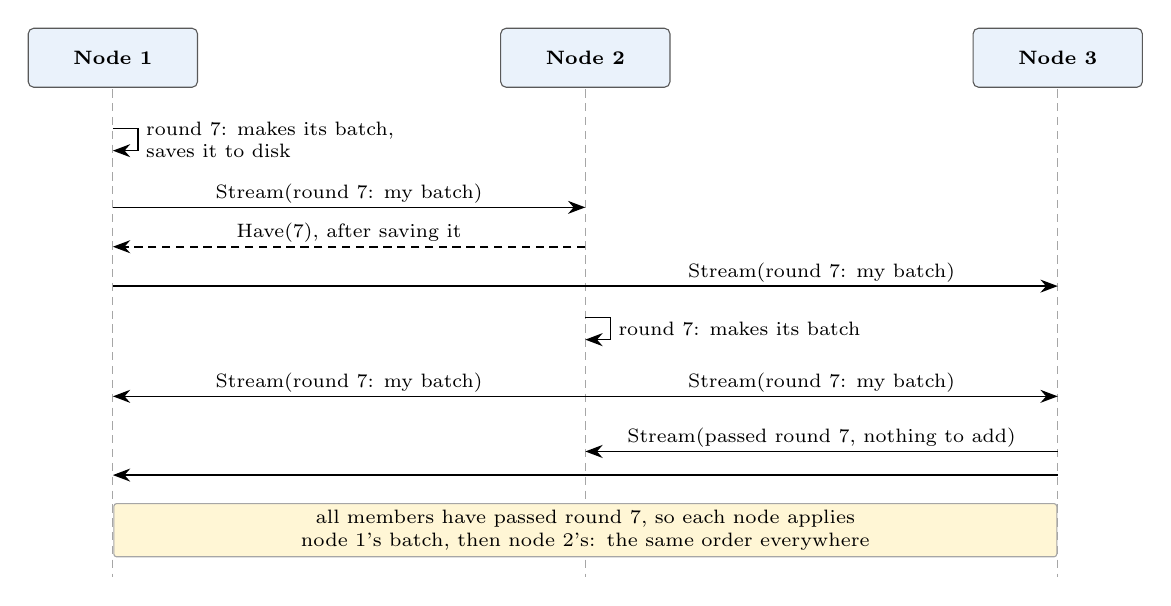
\begin{tikzpicture}[x=1cm,y=1cm]
  \seqactor{0}{Node 1}{-6.6}
  \seqactor{6.0}{Node 2}{-6.6}
  \seqactor{12.0}{Node 3}{-6.6}
  \seqself{0}{-0.9}{round 7: makes its batch,\\ saves it to disk}
  \seqmsg{0}{6.0}{-1.9}{Stream(round 7: my batch)}
  \seqrep{6.0}{0}{-2.4}{Have(7), after saving it}
  \seqmsg{0}{12.0}{-2.9}{}
  \node[mlabel] at (9.0,-2.9) {Stream(round 7: my batch)};
  \seqself{6.0}{-3.3}{round 7: makes its batch}
  \seqmsg{6.0}{12.0}{-4.3}{Stream(round 7: my batch)}
  \seqmsg{6.0}{0}{-4.3}{Stream(round 7: my batch)}
  \seqmsg{12.0}{6.0}{-5.0}{Stream(passed round 7, nothing to add)}
  \seqmsg{12.0}{0}{-5.3}{}
  \seqnote{6.0}{-6.0}{11.8}{all members have passed round 7, so each node applies node 1's batch, then node 2's: the same order everywhere}
\end{tikzpicture}
\caption{One round of the shared log. Each node sends only its own batches. A batch of node 1 is applied only after a peer has saved it, so anything a client is told is on at least two disks. Most replies are drawn only once.}
\label{fig:seq-rounds}
\end{figure}

\textbf{When a round is safe to apply.} Each node keeps, for every member, how far it holds that member's stream (\emph{covered}), and for every peer, how far that peer has saved its own stream (\emph{acked}). The \emph{frontier} is the highest round that is safe to apply: the lowest \emph{covered} over all members, and no higher than the highest \emph{acked} over the peers. Figure~\ref{fig:frontier} works through an example.

\begin{figure}[!htb]
\centering
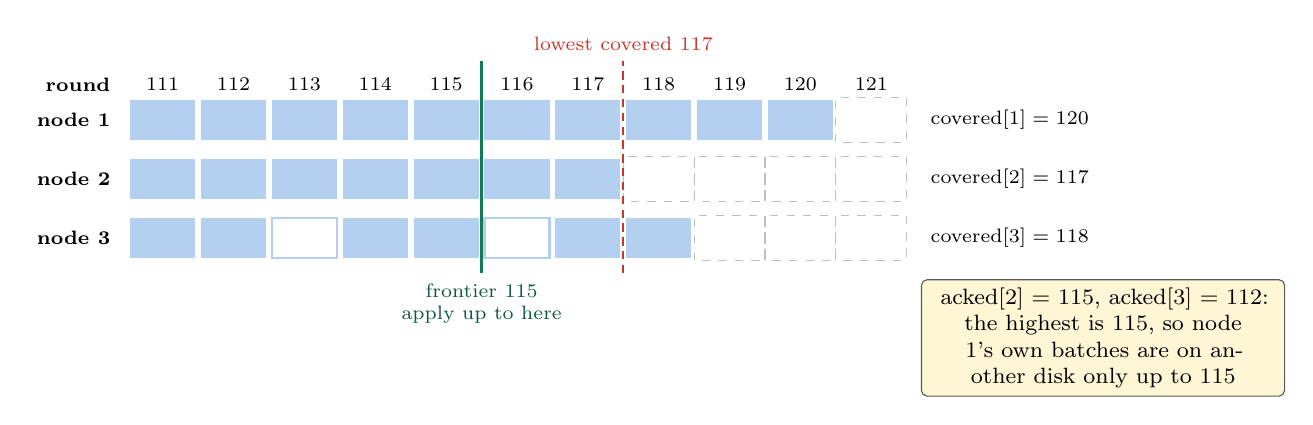
\begin{tikzpicture}[x=0.9cm,y=0.75cm]
  % header
  \foreach \r in {111,...,121} { \node[font=\scriptsize] at (\r-111+1.5,0.6) {\r}; }
  \node[font=\scriptsize\bfseries, anchor=east] at (0.9,0.6) {round};
  % rows: node, covered, empty rounds
  \foreach \n/\cov/\y in {1/120/0, 2/117/-1, 3/118/-2} {
    \node[font=\scriptsize\bfseries, anchor=east] at (0.9,\y) {node \n};
    \foreach \r in {111,...,121} {
      \pgfmathtruncatemacro{\c}{\r-111+1}
      \ifnum\r>\cov
        \draw[black!25, dashed] (\c,\y-0.38) rectangle (\c+1,\y+0.38);
      \else
        \fill[nodeblue!35] (\c+0.04,\y-0.34) rectangle (\c+0.96,\y+0.34);
      \fi
    }
    \node[font=\scriptsize, anchor=west] at (12.2,\y) {covered$[\n] = \cov$};
  }
  % empty rounds of node 3 (covered, no batch)
  \foreach \r in {113,116} {
    \pgfmathtruncatemacro{\c}{\r-111+1}
    \fill[white] (\c+0.04,-2.34) rectangle (\c+0.96,-1.66);
    \draw[nodeblue!35, line width=0.8pt] (\c+0.04,-2.34) rectangle (\c+0.96,-1.66);
  }
  % frontier and min covered lines
  \draw[very thick, mwgreen!70!black] (6,1.0) -- (6,-2.6) node[below, font=\scriptsize, align=center, text=mwgreen!50!black]{frontier 115\\ apply up to here};
  \draw[thick, badred, densely dashed] (8,-2.6) -- (8,1.0) node[above, font=\scriptsize, align=center, text=badred]{lowest covered 117};
  \node[box, fill=notefill, text width=4.4cm, anchor=north west] at (12.2,-2.7) {acked[2] = 115, acked[3] = 112:\\ the highest is 115, so node 1's own batches are on another disk only up to 115};
\end{tikzpicture}
\caption{The frontier on node 1, in an example from \texttt{docs/shared-log.md}. Filled cells are batches node 1 holds; outlined cells are rounds in which node 3 had nothing to say, which still count as passed. Everything up to round 115 is applied, sorted by round and then by node ID; nothing that arrives later can change that part of the order.}
\label{fig:frontier}
\end{figure}

\textbf{Why every node gets the same order.} Streams arrive in order over TCP. Once a node holds member $m$'s stream up to round 117, no batch of $m$ at or below 117 can still arrive. So every batch at or below the frontier is already here, and sorting them by round and then by node ID gives one order, which no later message can change. Every node sorts the same batches by the same key, and no node decides anything, so there is nothing to lead. The waiting batches are kept sorted by the pair (round, node), so the order comes from the key itself.

\textbf{Why the highest acked.} A node applies its own batch only after at least one peer has saved it. So whatever a client is told is on at least two disks, and survives the loss of any one node. This is the system's version of the rule ``commit, then reply''.

\textbf{On disk.} Each node appends to its own file, \texttt{node-<id>.rounds}. A save writes every waiting batch and then calls one disk sync for all of them, so a busy node saves more per sync, not more often. Since \dlog{D261} the file also records the order in which the node applied batches, saved before any client is answered, so that a restarted node can rebuild exactly what it told clients (Section~\ref{sec:multi}).

\textbf{Checking that the copies agree.} After every command each node updates its digest (Section~\ref{sec:datamodel}) and logs it at every 100th log index. The overnight series compared 69,715 of these checkpoints across nodes, and the kill runs 14,932 more. None differed.

\subsection{The team's code and the libraries}

The spec requires the two to be separated, and here the line is sharp. The libraries carry the log: tarpc makes the calls between nodes, bincode and serde encode the batches, and tokio runs the tasks, timers and file writes. Everything about the order is the team's own work: numbering batches into rounds, the sort by round and node ID, the frontier, agreeing to go on without a silent node, bringing a node back, and the log file. That is about 1,650 lines in \texttt{rounds.rs}, of which about 100 hold the ordering itself.

Before writing its own, the team looked for a library that orders a log with no leader (\dlog{D259}). \texttt{synevi} 0.1.0, an implementation of the Accord protocol, was compiled and run on the three node PCs. With no fault its digests matched; with one node stopped for 20 s the other two applied nothing for the whole fault, and all three ended with different digests. The \texttt{fantoch} implementations of EPaxos, Atlas and Tempo all stop at \texttt{todo!("recovery not implemented yet")}. AlephBFT and hbbft are built for attackers and, by their documentation, need four nodes to survive one failure. The others found have a leader (openraft, paxakos, OmniPaxos, Kafka) or carry messages with no agreed order (Zenoh, libp2p's gossipsub). The test's source and output are in \texttt{analysis/results/library-search/}.

% ==============================================================================================
\section{Fault model, failover and recovery}
\label{sec:faults}

\subsection{The faults and how we inject them}

\begin{table}[!htb]
\centering\small
\caption{The faults we handle, and how each is made in the experiments.}
\label{tab:faultmodel}
\begin{tabularx}{\linewidth}{@{}P{3.3cm}LL@{}}
\toprule
Fault & How it is made & What happens \\
\midrule
A node goes silent for 1 to 20 s & The fault election (Section~\ref{sec:faultelection}), or \texttt{ctl silence}. A \emph{fault gate} in the node's network code drops all peer and client traffic and keeps memory; control messages still pass (\dlog{D13}, \dlog{D22}) & The other two drop it after 1 s and go on; it catches up and is added back \\
A node's process dies & \texttt{kill -9}, then a restart; this stands in for turning a machine off (\dlog{D265}) & The same, but it first rebuilds from its own file \\
Two nodes fail, at once or in turn & Kills and silences in every order (Section~\ref{sec:kills}) & The last node answers provisionally until it can commit (\dlog{D261}, \dlog{D262}) \\
All three fail & Kills, back together or one at a time & Each rebuilds from its own file; the longest log goes first \\
Messages lost, late, doubled & UDP and Wi-Fi do this by themselves & Retries with the same ID; first result wins \\
\bottomrule
\end{tabularx}
\end{table}

We do not handle Byzantine faults, and we did not physically pull a plug. A kill stops a process at once, as a power cut would, but it cannot lose disk writes the way a real cut can. Section~\ref{sec:limits} states this as a limit.

\subsection{Failure detection}

Every node asks every peer ``are you alive?'' each 50 ms, and any answer counts (\code{node/heartbeat.rs}, \dlog{D41}, \dlog{D79}). A peer not heard from for 20 heartbeats, so 1 s, is suspected. The shared log also watches each member's stream, every 25 ms, and counts a member silent after the same 1 s (\code{run\_detector}). Each node decides for itself, and a guess can be wrong, since a slow node looks like a dead one \cite{chandra}. A wrong guess costs a drop and a rejoin, and never two different states, because the drop below needs two nodes to agree. The heartbeats are sent to every configured peer, never only to the current members, so that two nodes that dropped each other still hear each other again.

\subsection{Failover: going on without a silent node}
\label{sec:drop}

A silent member holds up every round, because the frontier needs its stream. So the other two agree to go on without it (Figure~\ref{fig:seq-drop}). The rule that keeps this safe is that a node gives at most one promise per view, so there can be only one next view (\dlog{D252}). Every batch the silent node could have applied is at or below the cut: it applies its own batches only once a peer has saved them, and both peers stopped counting its stream before they answered.

\begin{figure}[!htb]
\centering
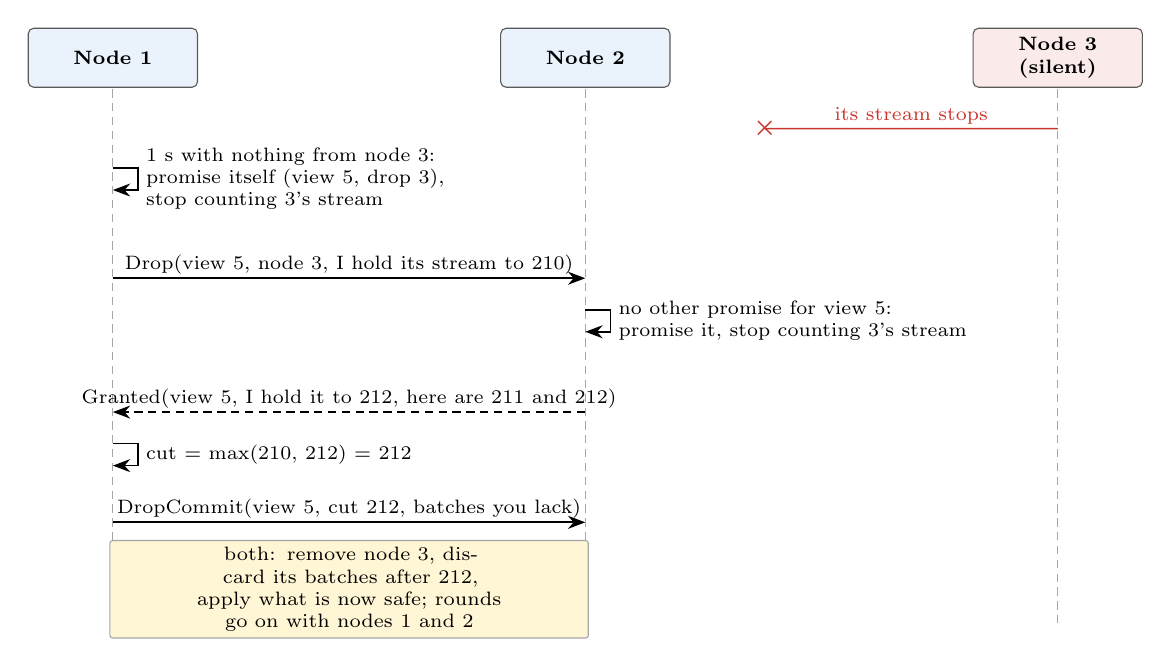
\begin{tikzpicture}[x=1cm,y=1cm]
  \seqactor{0}{Node 1}{-7.2}
  \seqactor{6.0}{Node 2}{-7.2}
  \seqactor[badred!10]{12.0}{Node 3\\(silent)}{-7.2}
  \seqlost{12.0}{6.0}{-0.9}{its stream stops}
  \seqself{0}{-1.4}{1 s with nothing from node 3:\\ promise itself (view 5, drop 3),\\ stop counting 3's stream}
  \seqmsg{0}{6.0}{-2.8}{Drop(view 5, node 3, I hold its stream to 210)}
  \seqself{6.0}{-3.2}{no other promise for view 5:\\ promise it, stop counting 3's stream}
  \seqrep{6.0}{0}{-4.5}{Granted(view 5, I hold it to 212, here are 211 and 212)}
  \seqself{0}{-4.9}{cut = max(210, 212) = 212}
  \seqmsg{0}{6.0}{-5.9}{DropCommit(view 5, cut 212, batches you lack)}
  \seqnote{3.0}{-6.75}{5.9}{both: remove node 3, discard its batches after 212,\\ apply what is now safe; rounds go on with nodes 1 and 2}
\end{tikzpicture}
\caption{Dropping a silent node (\code{try\_drop}, \code{on\_drop}, \code{install\_drop} in \texttt{rounds.rs}). A promise given to a peer is never taken back; without this rule, the lab PCs once made two different drops as the same view, and the digests split (\dlog{D252}).}
\label{fig:seq-drop}
\end{figure}

\subsection{Recovery: coming back}
\label{sec:rejoin}

The spec asks what state is copied, replayed or rebuilt, and how a returning node knows it is current. Figure~\ref{fig:seq-rejoin} shows the steps, and Table~\ref{tab:recovery} answers the questions.

\begin{figure}[!htb]
\centering
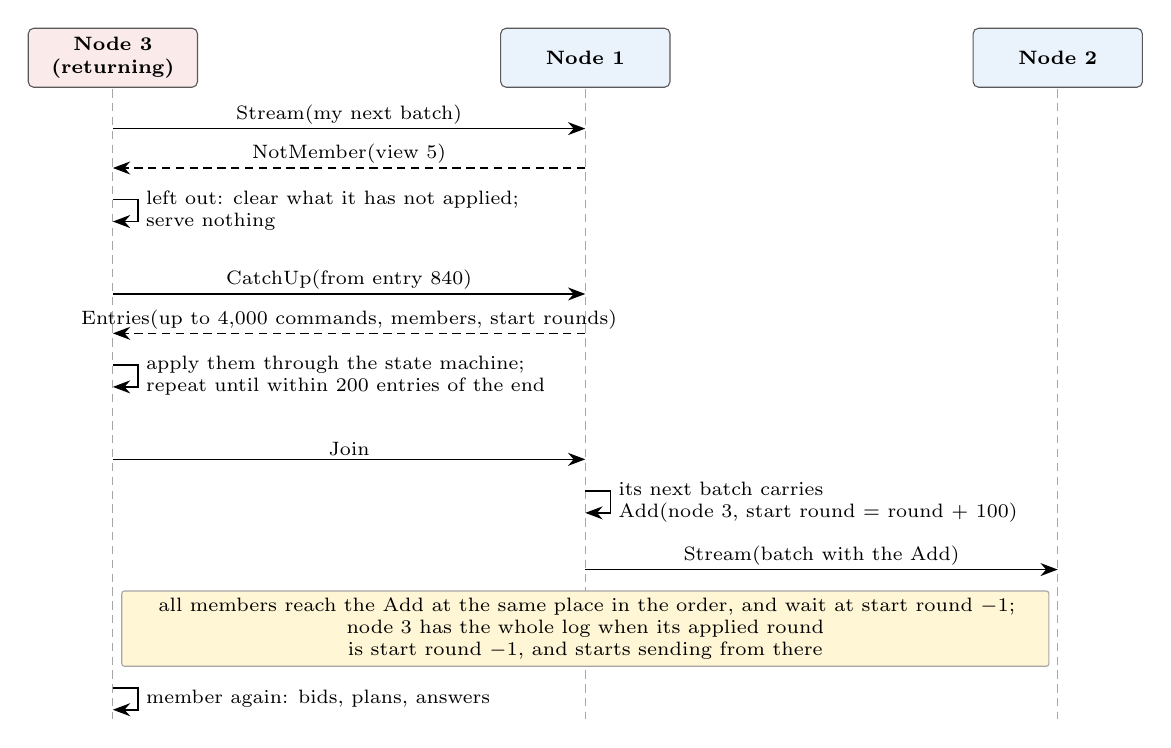
\begin{tikzpicture}[x=1cm,y=1cm]
  \seqactor[badred!10]{0}{Node 3\\(returning)}{-8.4}
  \seqactor{6.0}{Node 1}{-8.4}
  \seqactor{12.0}{Node 2}{-8.4}
  \seqmsg{0}{6.0}{-0.9}{Stream(my next batch)}
  \seqrep{6.0}{0}{-1.4}{NotMember(view 5)}
  \seqself{0}{-1.8}{left out: clear what it has not applied;\\ serve nothing}
  \seqmsg{0}{6.0}{-3.0}{CatchUp(from entry 840)}
  \seqrep{6.0}{0}{-3.5}{Entries(up to 4,000 commands, members, start rounds)}
  \seqself{0}{-3.9}{apply them through the state machine;\\ repeat until within 200 entries of the end}
  \seqmsg{0}{6.0}{-5.1}{Join}
  \seqself{6.0}{-5.5}{its next batch carries\\ Add(node 3, start round = round + 100)}
  \seqmsg{6.0}{12.0}{-6.5}{Stream(batch with the Add)}
  \seqnote{6.0}{-7.25}{11.6}{all members reach the Add at the same place in the order, and wait at start round $-1$;\\ node 3 has the whole log when its applied round is start round $-1$, and starts sending from there}
  \seqself{0}{-8.0}{member again: bids, plans, answers}
\end{tikzpicture}
\caption{A node comes back (\code{run\_catch\_up}, \code{on\_catch\_up}, \code{on\_join}). It is added through an entry in the shared order, so all members add it at the same place, and its new stream starts past the end of its old one (\dlog{D257}).}
\label{fig:seq-rejoin}
\end{figure}

\begin{table}[!htb]
\centering\small
\caption{The recovery protocol, against what the spec asks.}
\label{tab:recovery}
\begin{tabularx}{\linewidth}{@{}P{4.2cm}L@{}}
\toprule
The spec asks & Our answer \\
\midrule
What is copied, replayed or rebuilt? & First the node replays its own file, in the order it applied, which it saved before answering anyone (\dlog{D261}). Then a member sends what is missing, up to 4,000 commands a reply, and the node replays it through the same state machine. Its bids, suspicions and view are rebuilt from new traffic. One code path serves a silence and a restart. \\
How does it know it is current? & It asks to be added, and the members stop just before the round it starts at. It has the whole log exactly when its applied round is one before that start round, and only then does it send. A node whose log is not a start of the member's gets \code{Diverged}, writes \code{Reset} to its file, and takes the log again. \\
When does it take part again? & Its proposals are refused, and it bids, plans and answers nothing, until it is a member again (\dlog{D75}). This is checked again just before each reply, so a reply that was waiting during the fault stays quiet (\dlog{D136}). \\
\bottomrule
\end{tabularx}
\end{table}

Figure~\ref{fig:node-states} brings the pieces together as the life cycle of one node.

\begin{figure}[!htb]
\centering
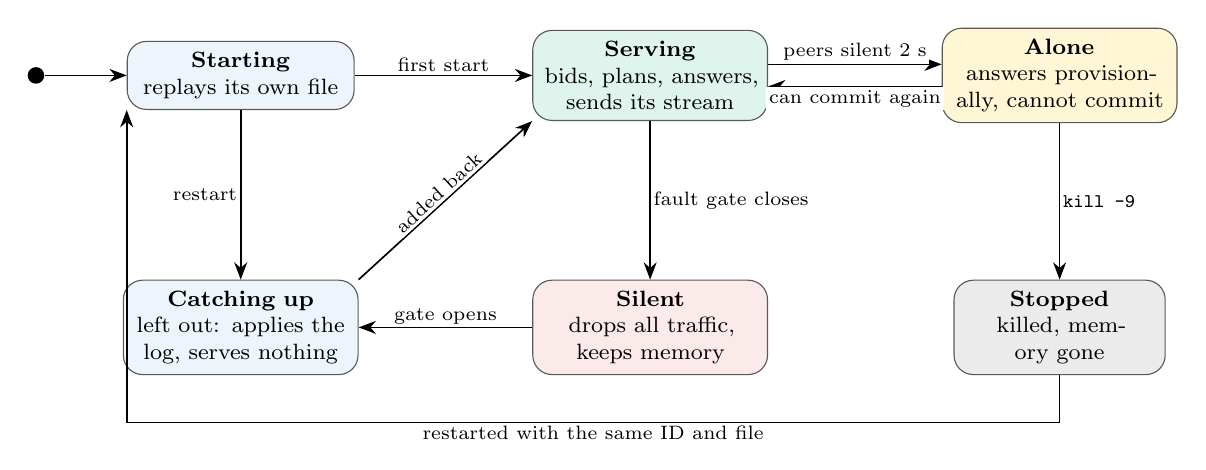
\begin{tikzpicture}[x=1cm,y=1cm]
  \node[sinit] (i) at (-1.4,0) {};
  \node[state, text width=2.6cm] (start) at (1.2,0) {\textbf{Starting}\\ replays its own file};
  \node[state, text width=2.7cm, fill=mwgreen!14] (serve) at (6.4,0) {\textbf{Serving}\\ bids, plans, answers, sends its stream};
  \node[state, text width=2.7cm, fill=notefill] (deg) at (11.6,0) {\textbf{Alone}\\ answers provisionally, cannot commit};
  \node[state, text width=2.7cm, fill=badred!10] (silent) at (6.4,-3.2) {\textbf{Silent}\\ drops all traffic, keeps memory};
  \node[state, text width=2.7cm] (catch) at (1.2,-3.2) {\textbf{Catching up}\\ left out: applies the log, serves nothing};
  \node[state, text width=2.4cm, fill=black!8] (dead) at (11.6,-3.2) {\textbf{Stopped}\\ killed, memory gone};
  \draw[flow] (i) -- (start);
  \draw[flow] (start) -- node[elabel, above]{first start} (serve);
  \draw[flow] (start) -- node[elabel, left]{restart} (catch);
  \draw[flow] ([yshift=4pt]serve.east) -- node[elabel, above]{peers silent 2 s} ([yshift=4pt]deg.west);
  \draw[flow] ([yshift=-4pt]deg.west) -- node[elabel, below]{can commit again} ([yshift=-4pt]serve.west -| serve.east);
  \draw[flow] (serve) -- node[elabel, right]{fault gate closes} (silent);
  \draw[flow] (silent) -- node[elabel, above]{gate opens} (catch);
  \draw[flow] (catch.north east) -- node[elabel, sloped, above]{added back} (serve.south west);
  \draw[flow] (deg) -- node[elabel, right]{\texttt{kill -9}} (dead);
  \draw[flow] (dead.south) -- ++(0,-0.6) -| node[elabel, pos=0.25, below]{restarted with the same ID and file} (start.south west);
\end{tikzpicture}
\caption{The life of one node. Any state can go to Stopped by a kill; only one such arrow is drawn. Alone is still serving, but its answers are labelled provisional (Section~\ref{sec:degraded}).}
\label{fig:node-states}
\end{figure}

\subsection{More than one failure}
\label{sec:multi}

The class notes ask what happens with one node off and another failed, leaving one server. Our first rotating rounds could not handle two failures close together: commits stopped for the rest of the run (\dlog{D261}). Raft would have carried on in some of these cases, as long as two nodes were up, but not with one. We fixed this in four steps on the final build. Each node now saves the order it applied before answering, and rebuilds from its own file when it restarts. A member with nobody else left takes a returning node straight back, with no vote, because in a view of two nothing commits without both, so the survivor holds everything that was applied. With nobody left, the node with the longest log goes first. Figure~\ref{fig:multi} is the decision a restarted node makes.

\begin{figure}[!htb]
\centering
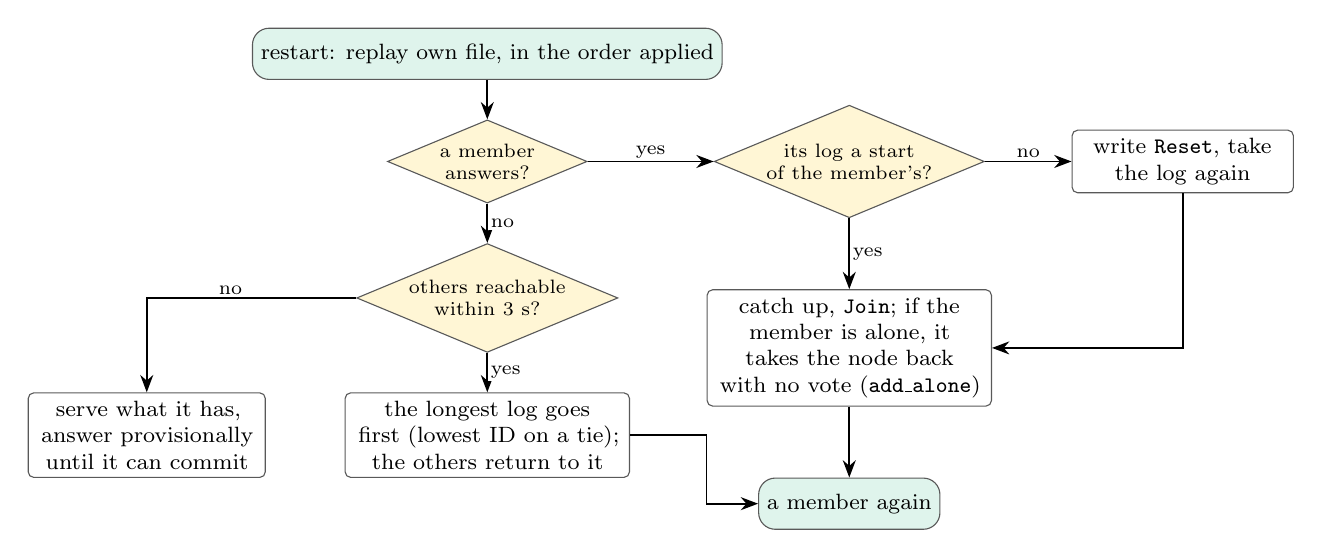
\begin{tikzpicture}[x=1cm,y=1cm, node distance=0.5cm]
  \node[fend] (s) {restart: replay own file, in the order applied};
  \node[fdec, below=of s] (m) {a member\\ answers?};
  \node[fdec, right=1.6cm of m] (pref) {its log a start\\ of the member's?};
  \node[fstep, right=1.1cm of pref, text width=2.6cm] (reset) {write \code{Reset}, take the log again};
  \node[fstep, below=0.9cm of pref, text width=3.4cm] (join) {catch up, \code{Join}; if the member is alone, it takes the node back with no vote (\code{add\_alone})};
  \node[fdec, below=of m] (others) {others reachable\\ within 3 s?};
  \node[fstep, below=of others, text width=3.4cm] (longest) {the longest log goes first (lowest ID on a tie); the others return to it};
  \node[fstep, left=1.0cm of longest, text width=2.8cm] (alone) {serve what it has, answer provisionally until it can commit};
  \node[fend, below=0.9cm of join] (back) {a member again};
  \draw[flow] (s) -- (m);
  \draw[flow] (m) -- node[elabel, above]{yes} (pref);
  \draw[flow] (pref) -- node[elabel, above]{no} (reset);
  \draw[flow] (reset) |- (join.east);
  \draw[flow] (pref) -- node[elabel, right]{yes} (join);
  \draw[flow] (m) -- node[elabel, right]{no} (others);
  \draw[flow] (others) -- node[elabel, right]{yes} (longest);
  \draw[flow] (others.west) -| node[elabel, pos=0.3, above]{no} (alone.north);
  \draw[flow] (longest.east) -- (longest.east -| join.west) |- (back.west);
  \draw[flow] (join) -- (back);
\end{tikzpicture}
\caption{What a node does after a restart (\code{run\_catch\_up}, \dlog{D261}). A node that cannot commit yet answers provisionally, so a client is never left with silence for long.}
\label{fig:multi}
\end{figure}

\subsection{One node left: provisional answers}
\label{sec:degraded}

A single node cannot commit, because the shared log needs a peer to save each batch. Waiting would leave the three client PCs with no answers, which is the opposite of what the class notes ask for. So a node alone answers anyway, with a plan it labels \code{Provisional}, and records it properly once a peer is back (\dlog{D120}, \dlog{D262}). This breaks our rule ``commit, then reply'', and we chose it knowingly: it trades consistency for availability in this one case, as the spec allows for speculative actions that are ``clearly labeled and reconciled''.

When a peer returns, the lone node replays its provisional plans through the shared log, and the first result recorded still wins. A provisional answer can therefore turn out to differ: another node may have planned the same report first, or the responder may have been taken. The client is not told (\dlog{D122}). In T2, with 300 responders, about 98\% of provisional answers ended differently on record (Section~\ref{sec:kills}), so a provisional answer here means ``someone will come'' rather than ``this responder will come''. Its answers are held in memory until replayed, so killing the lone node loses them.

\subsection{Consistency model}
\label{sec:consistency}

The spec asks for a consistency model for incidents, presence, resources, leases and offline changes. Phase 1 has incidents and responders; the rest belongs to Phase 2.

\begin{itemize}
  \item \textbf{Writes are totally ordered.} Every change to incidents and responders is a command in the shared log, applied by every node in the same order by a deterministic state machine. So all nodes pass through the same states, and equal digests at the same index show it.
  \item \textbf{An answer is durable before it is sent.} A node answers only after its result is applied, and it applies its own batch only after a peer saved it. The one exception is the labelled provisional answer above.
  \item \textbf{Conflicts are settled by order, not by clocks.} Two plans for the same report: the first in the order wins, and the second gets it back. Two reports wanting the same responder: the first in the order holds it, and the second chooses again at apply, the same way on every node (\dlog{D241}). No vector clocks are needed, because there is one order.
  \item \textbf{Reads are local.} A node answers a retry or a status read from its own copy, which may be a few rounds behind another node's. A returning node reads nothing until it is current.
  \item \textbf{No clock decides anything replicated.} The state machine reads no clock (\dlog{D30}). ``Too old'' is judged from the age the client states, so it never compares two machines' clocks (\dlog{D143}).
\end{itemize}

% ==============================================================================================
\section{Results}
\label{sec:results}

All results in this section come from the six lab PCs with rotating rounds. Tables not marked otherwise are from the overnight series on the overnight build, 5 runs per cell; results from the final build are marked. Section~\ref{sec:method} describes how the runs were made and counted.

\begin{table}[!htb]
\centering\small
\caption{Every run, in total.}
\label{tab:totals}
\begin{tabular}{@{}lrr@{}}
\toprule
 & Overnight series & Kill runs (final build) \\
\midrule
Runs & 157 & 49 \\
Requests sent & 199,481,205 & 50,587,740 \\
Answered & 199,464,878 & 48,331,376 \\
Gave up after all retries & 16,327 & 2,256,364 \\
Unaccounted for & 0 & 0 \\
Digest checkpoints compared & 69,715 & 14,932 \\
Digest mismatches & 0 & 0 \\
\bottomrule
\end{tabular}
\end{table}

``Gave up'' is not a failure of the system above what the nodes left can carry: with one node left there is about a third of the capacity, and with none, nobody can answer. The checks that must always hold are 0 unaccounted and 0 digest mismatches.

\subsection{Load balancing: scenarios 1 and 2}
\label{sec:lb}

\textbf{Scenario 1, load changing.} Five runs of 240 s: 1,000 reports a second, then 5,000, then 9,000, then back to 1,000, from all three client PCs, with planning work 1000. Every node kept winning at every load, each between 31.4\% and 34.5\% (Table~\ref{tab:s1}, Figure~\ref{fig:s1}). The bids followed the load, from an expected wait of about 4,400 $\mu$s to about 56,000 $\mu$s and back. Since the PCs are the same model and the load is even, even shares are the fair result. The winner is chosen again for every report, so this is not nodes taking turns. Scenario 2 shows what happens when one node really is busier.

\begin{table}[!htb]
\centering\small
\caption{Scenario 1: share of reports each node won, and its mean bid in $\mu$s of expected wait.}
\label{tab:s1}
\begin{tabular}{@{}lrrrrrrr@{}}
\toprule
Load & Answers/s & Node 1 & Node 2 & Node 3 & Bid 1 & Bid 2 & Bid 3 \\
\midrule
1,000/s & 999 & 33.8\% & 33.1\% & 33.2\% & 4,390 & 4,390 & 4,402 \\
5,000/s & 4,998 & 34.5\% & 31.9\% & 33.6\% & 24,019 & 24,255 & 23,969 \\
9,000/s & 8,998 & 34.2\% & 31.4\% & 34.4\% & 55,891 & 56,554 & 55,863 \\
back to 1,000/s & 999 & 33.7\% & 33.1\% & 33.1\% & 4,410 & 4,427 & 4,452 \\
\bottomrule
\end{tabular}
\end{table}

\begin{figure}[!htb]
\centering
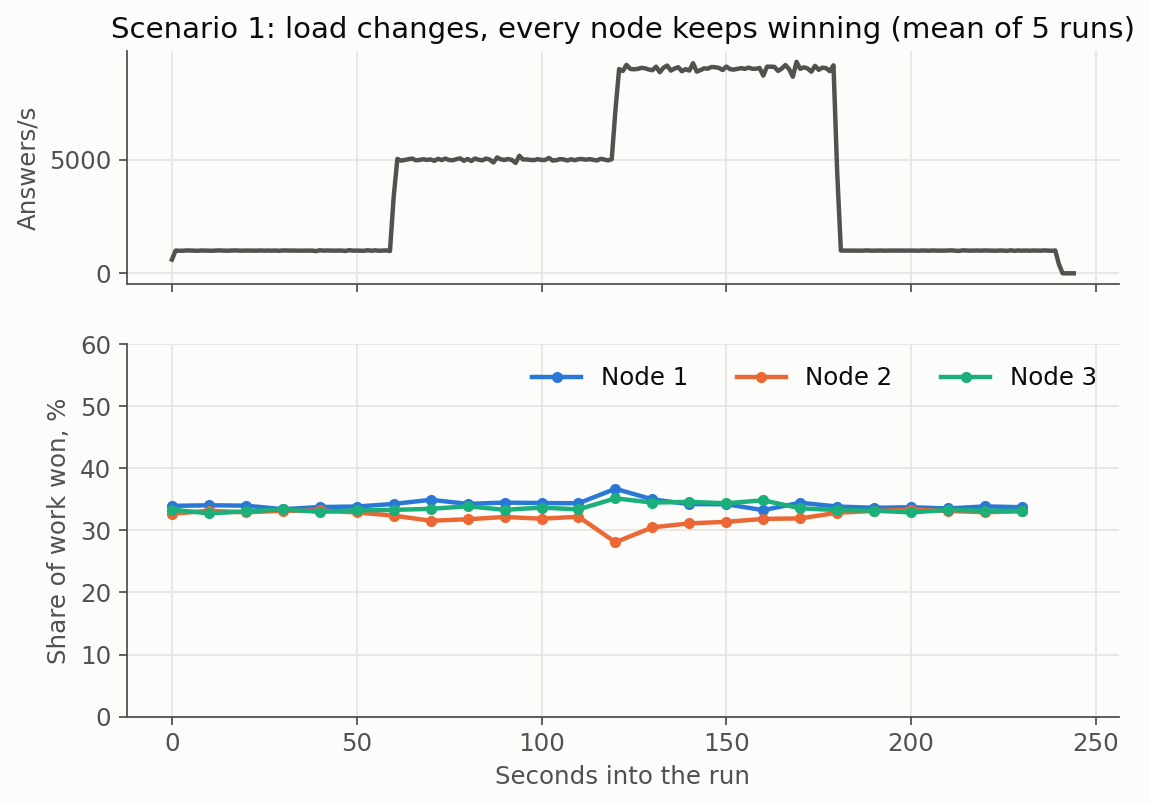
\includegraphics[width=0.82\linewidth]{figures/scenario1.png}
\caption{Scenario 1: shares and bids as the load steps up and down, mean of 5 runs.}
\label{fig:s1}
\end{figure}

\textbf{Scenario 2, one node made slow.} Five runs of 180 s at 3,000 reports a second. From 60 s to 120 s one node's planning work goes from 1000 to 5000, so a plan takes about 20 ms instead of 4 ms; the slowed node changes between runs. The system's score, expected wait, is compared with a queue-only score and with a control run where nothing is slowed (Table~\ref{tab:s2}, Figure~\ref{fig:s2}).

\begin{table}[!htb]
\centering\small
\caption{Scenario 2: share of the slowed node and its bid, before, during and after the slowdown.}
\label{tab:s2}
\begin{tabular}{@{}llrrrr@{}}
\toprule
Score & Phase & Slowed node won & Each other node & Slowed node's bid & Others' bid \\
\midrule
Expected wait (in use) & before & 33.4\% & 33.3\% & 13,831 & 13,791 \\
 & slowed & \textbf{4.9\%} & 47.6\% & 30,393 & 17,883 \\
 & after & 33.3\% & 33.3\% & 13,980 & 13,963 \\
Queue length only & before & 33.5\% & 33.3\% & 88 & 88 \\
 & slowed & 25.2\% & 37.4\% & 93 & 94 \\
 & after & 33.6\% & 33.2\% & 88 & 88 \\
Control, nothing slowed & slowed & 34.7\% & 32.7\% & 13,852 & 13,912 \\
\bottomrule
\end{tabular}
\end{table}

\begin{figure}[!htb]
\centering
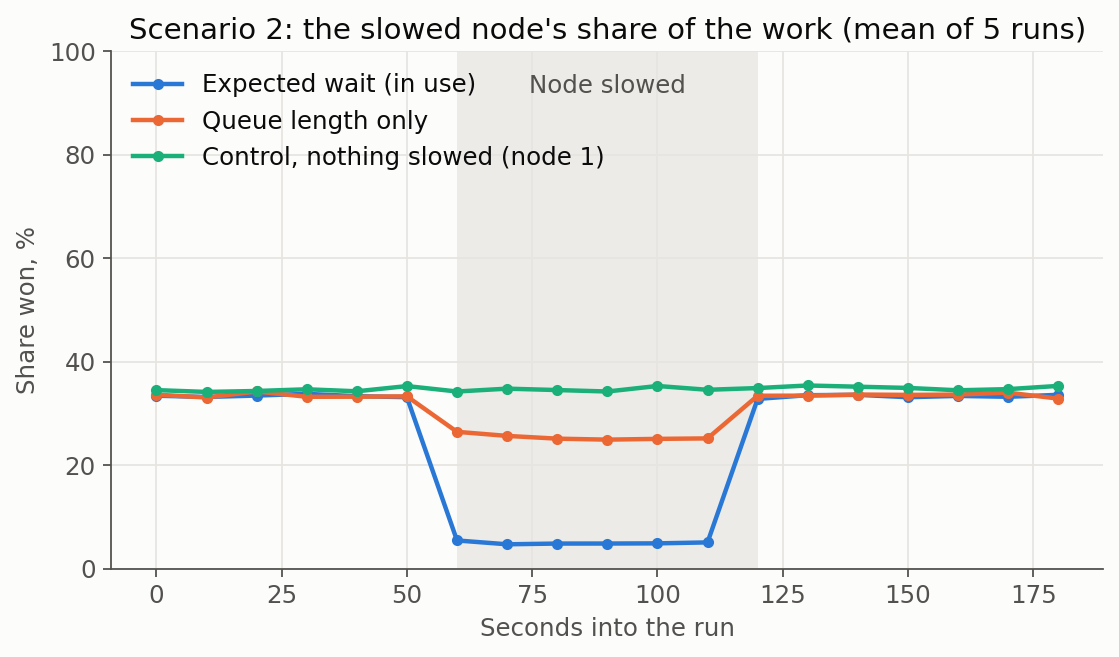
\includegraphics[width=0.82\linewidth]{figures/scenario2.png}
\caption{Scenario 2: the slowed node's share, under the expected-wait score, a queue-only score and the control.}
\label{fig:s2}
\end{figure}

When one node is slowed, its bid more than doubles and its share falls from 33.4\% to 4.9\%, while each of the others takes 47.6\%. When the slowdown ends it is back at 33.3\%. Service does not suffer: the median latency was 136 ms, the same as the control, and nobody gave up. A queue-only score reacts far less, to 25.2\%, because its bids hardly change (93 against 94): at this load a slow plan does not show up in the queue. This is the measured reason for using expected wait.

\subsection{Server failure: scenario 3}
\label{sec:s3}

A node stops answering for 20 s, 45 s into a 150 s run, under load from all three client PCs. The victim changes between runs. Table~\ref{tab:s3} and Figure~\ref{fig:s3} show the results at six loads.

\begin{table}[!htb]
\centering\small
\caption{Scenario 3: a 20 s fault under load, 5 runs per row. ``Dropped'' is when the others went on without the node. The in-flight columns count the reports the silent node had won in its last second: how many were still unanswered 0.3 s after the fault, how many of those the others planned again, and how many already had the silent node's plan in the log.}
\label{tab:s3}
\footnotesize\setlength{\tabcolsep}{4.5pt}
\begin{tabular}{@{}rrrrrrrrr@{}}
\toprule
Offered/s & Planning work & Answers/s during & p99 during, ms & Dropped, ms & Unanswered & Replanned & In log & Gave up \\
\midrule
1,000 & 1000 & 999 & 942 & 1,037 & 23 & 12 & 11 & 0 \\
5,000 & 1000 & 5,005 & 1,535 & 1,043 & 117 & 42 & 75 & 0 \\
8,000 & 1000 & 8,007 & 1,624 & 1,036 & 297 & 82 & 215 & 0 \\
10,000 & 0 & 10,002 & 2,075 & 1,048 & 405 & 23 & 382 & 0 \\
20,000 & 0 & 20,022 & 2,381 & 1,065 & 669 & 9 & 660 & 0 \\
30,000 & 0 & 29,992 & 2,688 & 1,054 & 1,772 & 47 & 1,725 & 12,303 \\
\bottomrule
\end{tabular}
\end{table}

\begin{figure}[!htb]
\centering
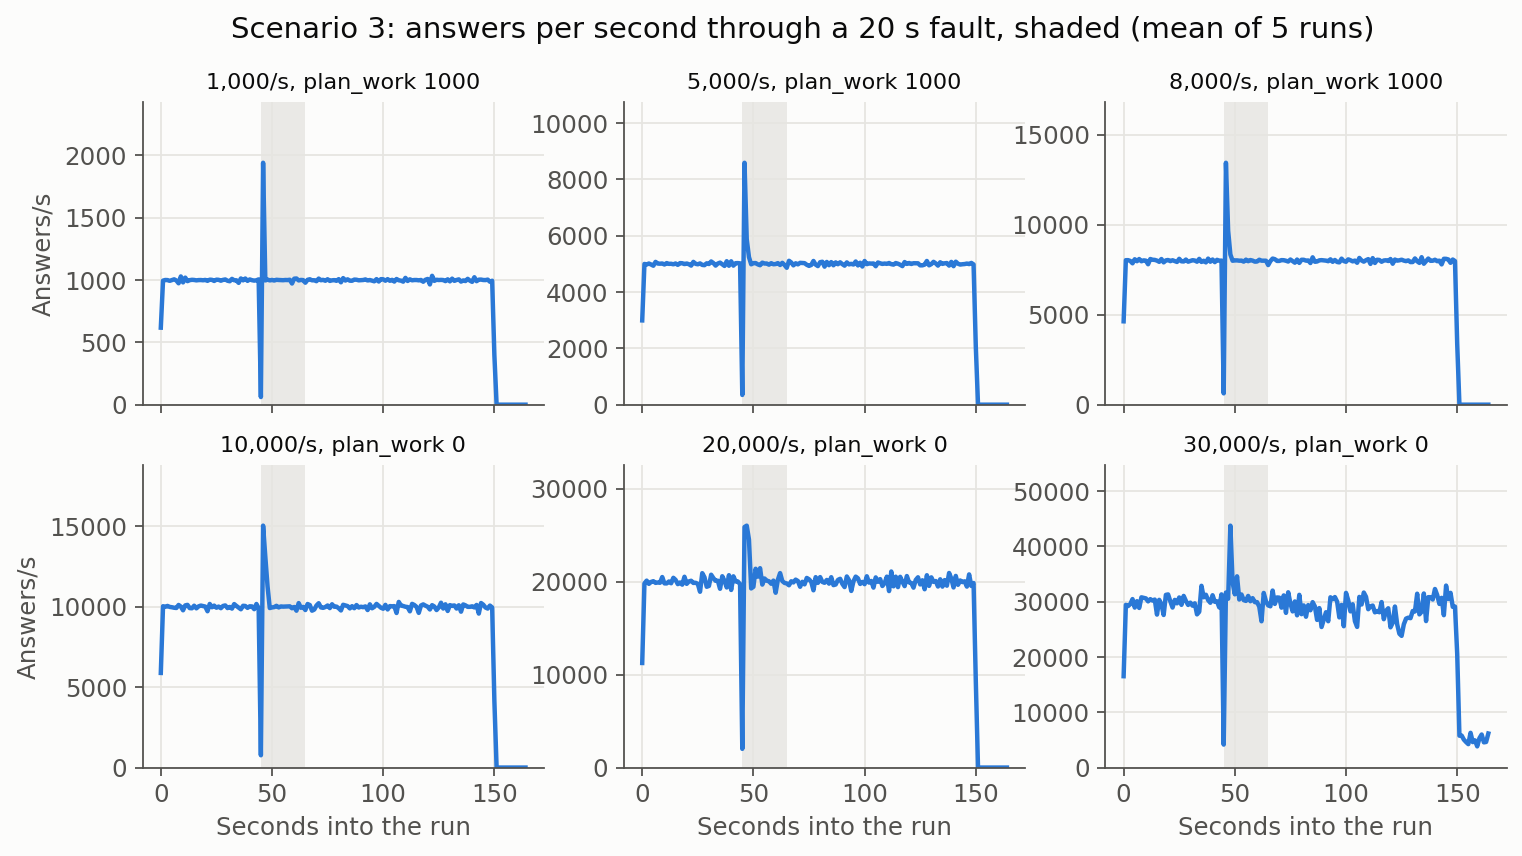
\includegraphics[width=0.9\linewidth]{figures/scenario3.png}
\caption{Scenario 3: answers per second through a 20 s fault (shaded), mean of 5 runs.}
\label{fig:s3}
\end{figure}

\begin{itemize}
  \item \textbf{Failover time} was about 1.04 s at every load, from 1,036 ms to 1,065 ms. It is the detection time, and it does not grow with load.
  \item \textbf{During the fault}, answers fall almost to nothing for about a second, then a burst clears the backlog, and the rate stays at the offered rate for the rest of the fault. The burst is why the ``during'' column equals the offered rate, and the reports caught in that second are why p99 rises.
  \item \textbf{Requests in flight} were all accounted for. Of the reports the silent node had won in its last second, most were answered before it stopped. Of those still unanswered 0.3 s later, at 10,000 a second, 23 were planned again by the others, and 382 already had the silent node's result in the log, so a peer gave that answer.
  \item \textbf{Transparency.} Across 6,879,602 answers given from 2 s into a fault to its end, none came from the silent node. Clients were not told of any failure, and needed no change.
  \item \textbf{The limit.} At 30,000 a second the system is at its edge: in 2 of 5 runs reports gave up, 12,233 and 70.
\end{itemize}

\subsection{Server recovery: scenario 4}
\label{sec:s4}

The same runs give the recovery of the returning node, together with a 5 s fault at 10,000 a second and runs where the process was killed and started 30 s later (Table~\ref{tab:s4}, Figure~\ref{fig:s4}). ``Caught up'' is when it had applied the whole log; ``member again'' is when its proposals were accepted again, which ends recovery.

\begin{table}[!htb]
\centering\small
\caption{Scenario 4: recovery and convergence, 5 runs per row, mean $\pm$ 95\% interval.}
\label{tab:s4}
\begin{tabular}{@{}lrrrrr@{}}
\toprule
Fault, load & Planning work & Caught up, ms & Member again, ms & Mismatches & One digest at the end \\
\midrule
20 s, 1,000/s & 1000 & 290 $\pm$ 73 & 800 $\pm$ 75 & 0 & 5 of 5 \\
20 s, 5,000/s & 1000 & 1,247 $\pm$ 319 & 1,820 $\pm$ 364 & 0 & 5 of 5 \\
20 s, 8,000/s & 1000 & 2,078 $\pm$ 557 & 2,848 $\pm$ 733 & 0 & 5 of 5 \\
20 s, 10,000/s & 0 & 2,801 $\pm$ 637 & 3,632 $\pm$ 809 & 0 & 5 of 5 \\
20 s, 20,000/s & 0 & 6,744 $\pm$ 1,628 & 10,488 $\pm$ 4,118 & 0 & 5 of 5 \\
20 s, 30,000/s & 0 & 14,384 $\pm$ 3,246 & 73,320 $\pm$ 34,451 & 0 & 5 of 5 \\
5 s, 10,000/s & 0 & 875 $\pm$ 162 & 1,414 $\pm$ 199 & 0 & 5 of 5 \\
killed, 5,000/s & 1000 & 6,023 $\pm$ 1,328 & 6,000 $\pm$ 1,324 & 0 & 5 of 5 \\
killed, 10,000/s & 0 & 11,994 $\pm$ 3,219 & 11,958 $\pm$ 3,235 & 0 & 5 of 5 \\
\bottomrule
\end{tabular}
\end{table}

\begin{figure}[!htb]
\centering
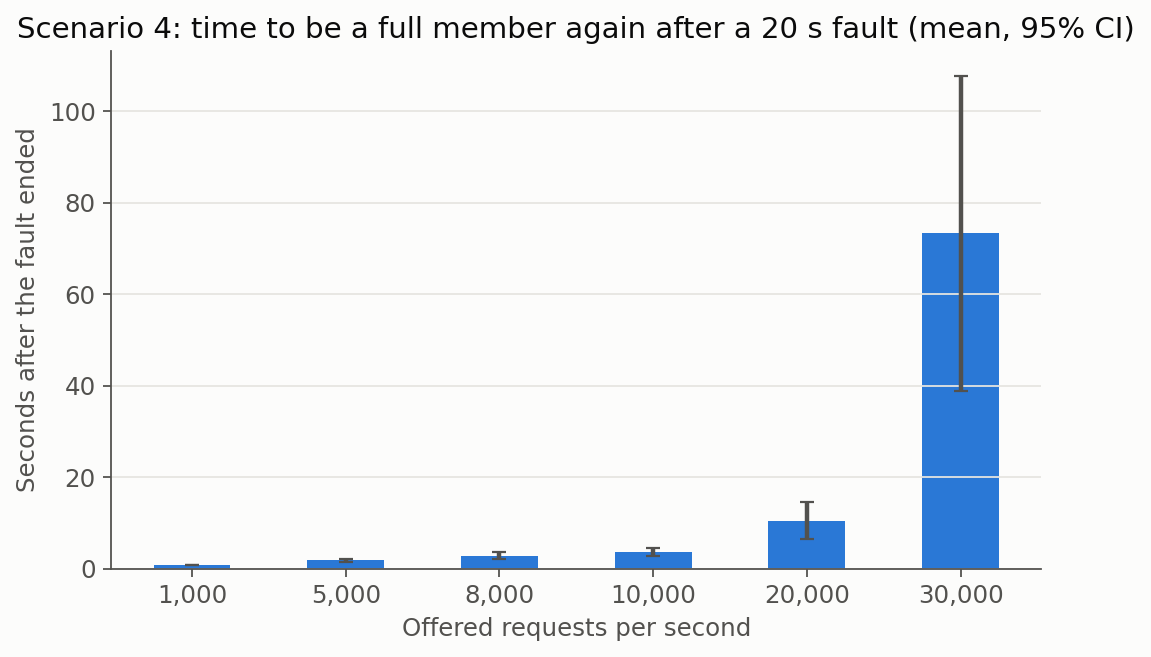
\includegraphics[width=0.78\linewidth]{figures/scenario4.png}
\caption{Scenario 4: time until the returning node was a member again, by load.}
\label{fig:s4}
\end{figure}

Recovery takes longer as load rises, because the node replays what it missed while new commands keep arriving: 0.8 s at 1,000 a second, 3.6 s at 10,000 and 10.5 s at 20,000. At 30,000 it took 73 s on average, most likely because little capacity is left on the air to catch up with. A shorter fault is quicker: 1.4 s after a 5 s fault at 10,000 a second, against 3.6 s after a 20 s one. A killed process has nothing in memory and rebuilds everything, in 6 s at 5,000 a second and 12 s at 10,000. Every run ended with one digest on all three nodes, within about 2 s of the load ending on average, and no checkpoint ever differed.

\textbf{Faults the nodes elect themselves.} With the fault election running every 20 to 30 s for 5 minutes at 3,000 a second, 5 runs gave 47 elected faults and 4,720,275 requests, with nobody giving up and 0 mismatches in 4,911 checkpoints. Over the 47 faults, the others dropped the silent node in a median of 1,018 ms (at most 1,036 ms), and it caught up with the log in a median of 428 ms after its silence ended (at most 1,141 ms).

\subsection{Two and three nodes killed}
\label{sec:kills}

This goes beyond one failure at a time, on the final build. Each run is 90 s with 10 s of warm-up, and both the nodes and the times are random: the first kill comes 15 to 30 s in, nodes stay down 5 to 20 s, and the last return leaves at least 25 s to recover. After each run, a checking tool lists what each node's own file applied, and every answer a client got is looked for there. Table~\ref{tab:kills} gives the cases at 10,000 reports a second with planning, the system's target load. The same cases were also run at 300, 15,000 and 20,000 a second.

\begin{table}[!htb]
\centering\small
\caption{Kills at 10,000 reports a second with planning, 3 runs per case, on the final build. Ranges are the lowest and highest run. Every case had 0 unaccounted and 0 digest mismatches.}
\label{tab:kills}
\begin{tabularx}{\linewidth}{@{}LrrP{2.6cm}P{2.0cm}P{2.0cm}@{}}
\toprule
Case & Answers/s & Answered & Gave up per run & Longest with no answer & Longest with no commit \\
\midrule
One node & 10,000 & 100.0\% & 0 & 0.9 to 1.0 s & 0.9 to 1.0 s \\
Two; first killed returns first & 9,848 & 96.7 to 99.6\% & 3,234 to 29,895 & 1.0 to 3.7 s & 1.6 to 8.7 s \\
Two; last killed returns first & 9,778 & 96.5 to 100.0\% & 0 to 31,219 & 1.4 to 1.9 s & 1.4 to 9.1 s \\
Two at the same moment & 9,555 & 93.2 to 97.3\% & 23,978 to 61,240 & 1.3 to 1.4 s & 8.1 to 10.9 s \\
Second killed just after first returns & 10,000 & 100.0\% & 0 & 1.0 s & 1.0 s \\
All three, back together & 9,197 & 86.4 to 97.3\% & 24,639 to 121,952 & 8.6 to 21.4 s & 8.6 to 21.4 s \\
All three, back one at a time & 8,567 & 83.3 to 87.5\% & 112,501 to 150,689 & 11.4 to 19.4 s & 11.4 to 19.4 s \\
\bottomrule
\end{tabularx}
\end{table}

Figure~\ref{fig:bynodes} shows the shape of these runs: what the cloud delivered with three, two, one and no nodes up. With one node up, most answers are provisional, which is the lone node answering on its own; when all are down, the few answers left come from the moments of rejoining.

\begin{figure}[!htb]
\centering
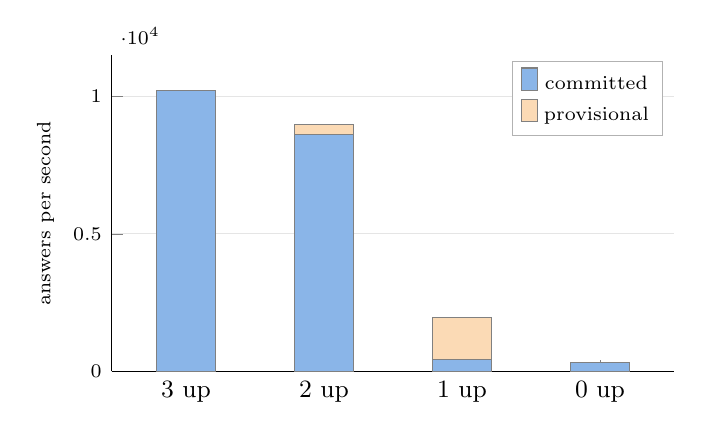
\begin{tikzpicture}
\begin{axis}[
  ybar stacked, bar width=0.75cm, width=0.72\linewidth, height=5.6cm,
  ymin=0, ymax=11500, ylabel={answers per second},
  symbolic x coords={3 up, 2 up, 1 up, 0 up}, xtick=data,
  yticklabel style={/pgf/number format/fixed, /pgf/number format/1000 sep={,}, font=\scriptsize},
  xticklabel style={font=\small}, label style={font=\scriptsize},
  legend style={font=\scriptsize, at={(0.98,0.98)}, anchor=north east, draw=black!30},
  axis lines*=left, ymajorgrids, grid style={black!10}, enlarge x limits=0.18,
]
\addplot[fill=nodeblue!55, draw=black!50] coordinates {(3 up,10208) (2 up,8621) (1 up,441) (0 up,337)};
\addlegendentry{committed}
\addplot[fill=notefill!80!clientorange, draw=black!50] coordinates {(3 up,0) (2 up,363) (1 up,1534) (0 up,0)};
\addlegendentry{provisional}
\end{axis}
\end{tikzpicture}
\caption{Answers per second by how many nodes were up, in the kill runs at 10,000 a second with planning, on the final build: 44, 27, 12 and 6 stretches of at least 3 s. One node alone answers about 2,000 a second, a bit under the third of the capacity it holds; stretches with three up include working off the backlog.}
\label{fig:bynodes}
\end{figure}

\textbf{The lab guide's T1 and T2 on the final build}, with 300 users: T1, a node killed and back, answered all 81,647 reports with a median of 98 ms, and nobody gave up. T2, one node killed and one silenced so that one is left for all three client PCs, answered all reports in each of its 3 runs, with about 4,850 provisional answers per run and equal digests at the end.

\subsection{Scale and stress: scenario 9}
\label{sec:stress}

The offered rate was raised until the answers stopped keeping up, with two planning loads: planning work 0, which tests what the protocol and the network can carry, and planning work 1000, about 4 ms of planning per report, which gives the real computing load the spec requires. Each run is 75 s, of which 60 s are measured, 5 runs per rate. A run ``held'' if it answered at least 99\% of the offered rate, nobody gave up, and p99 stayed under 3 s. This test is the team's own, not a requirement; 3 s allows an answer that needed the client's 2 s retry.

\begin{table}[!htb]
\centering\small
\caption{The stress series, mean of 5 runs. Cores is the mean CPU use per node.}
\label{tab:stress}
\begin{tabular}{@{}rrcrrrrrr@{}}
\toprule
Offered/s & Planning work & Held & Answered/s & Gave up & p50 ms & p95 ms & p99 ms & Cores \\
\midrule
5,000 & 0 & 5 of 5 & 5,004 & 0 & 137 & 180 & 227 & 0.3 \\
10,000 & 0 & 5 of 5 & 9,994 & 0 & 146 & 206 & 268 & 0.5 \\
20,000 & 0 & 5 of 5 & 20,007 & 0 & 171 & 317 & 451 & 0.9 \\
30,000 & 0 & 5 of 5 & 30,020 & 0 & 218 & 427 & 631 & 1.4 \\
33,000 & 0 & 3 of 5 & 32,197 & 5 & 271 & 1,723 & 3,814 & 1.5 \\
35,000 & 0 & 3 of 5 & 34,215 & 1,799 & 482 & 3,763 & 6,552 & 1.6 \\
36,000 & 0 & 1 of 5 & 34,070 & 2,160 & 633 & 5,569 & 10,323 & 1.6 \\
\midrule
1,000 & 1000 & 5 of 5 & 999 & 0 & 130 & 160 & 213 & 1.1 \\
5,000 & 1000 & 5 of 5 & 5,004 & 0 & 141 & 182 & 232 & 5.4 \\
10,000 & 1000 & 5 of 5 & 9,999 & 0 & 160 & 226 & 349 & 13.1 \\
12,000 & 1000 & 5 of 5 & 11,995 & 0 & 173 & 310 & 391 & 16.8 \\
14,000 & 1000 & 0 of 5 & 13,705 & 60 & 803 & 1,887 & 3,964 & 20.2 \\
\bottomrule
\end{tabular}
\end{table}

\begin{figure}[!htb]
\centering
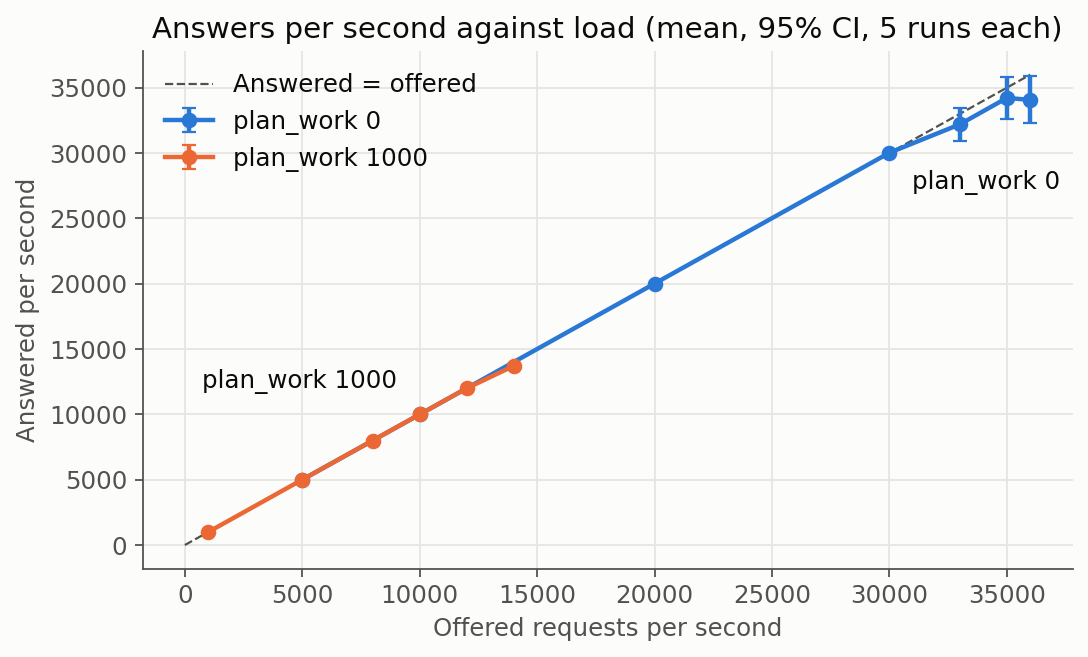
\includegraphics[width=0.49\linewidth]{figures/throughput.png}\hfill
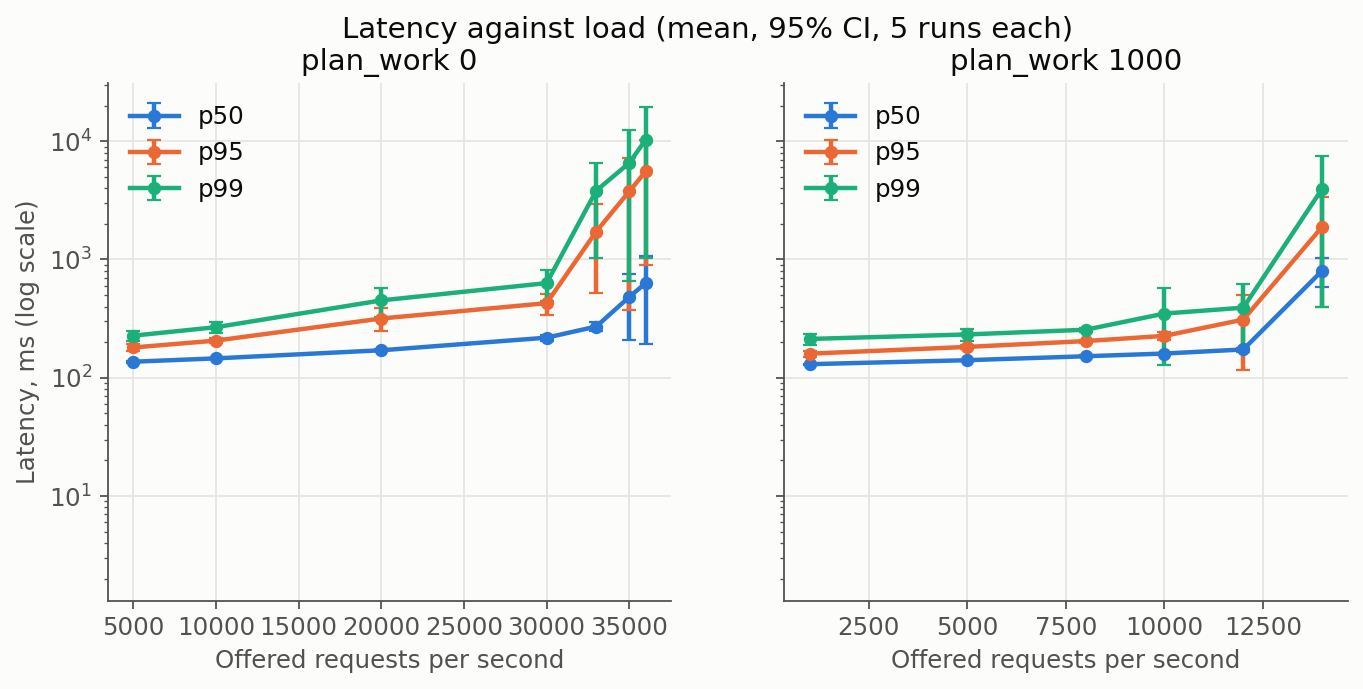
\includegraphics[width=0.49\linewidth]{figures/latency.png}
\caption{Throughput (left) and latency (right) against the offered rate, for both planning loads, mean of 5 runs.}
\label{fig:stress}
\end{figure}

\textbf{The ceiling} is 30,000 reports a second with almost no planning, held in all 5 runs and in a 5-minute hold (9,449,055 requests, p99 562 ms), and 12,000 a second with the planning load, held in all 5 runs. Above 30,000, results depend on the run. Answers per second stop rising at about 34,000.

\textbf{What limits it.} With planning, it is the CPU: the cores used per node rise with the rate, to about 20 at 14,000 a second, which is the size of the planning pool. Without planning, each node used under 2 cores above 30,000 a second, while elections saw fewer bids and retries rose. Fewer and smaller packets moved the ceiling up, which also points at the shared Wi-Fi. Air time was not measured directly.

\textbf{Where the time goes.} Latency is measured by the client, from when a report was due to go. Most of the median is the 60 ms election window, then the shared log. A p99 just over 2,000 ms means some answers needed the 2 s retry.

\textbf{Clients scale too.} The same 10,000 reports a second from one, two or three client PCs gave the same answered rate, with medians of 120, 130 and 146 ms, so the client PCs were not the limit. On the final build, 333 and 1,000 simulated users per client PC (999 and 3,000 in all, closed loop) answered every report.

\textbf{On a busier network.} At midday on November 5 the network was much busier. The final build answered all of 10,000 and 15,000 reports a second in 3 of 3 runs each, but at 30,000 it answered only 25,160 to 26,046 a second. To see whether the build or the network caused this, the overnight build was run again at midday at 30,000 a second, and it fell the same way. So 30,000 and above need a stable network, and the failure results are reported at 10,000 and 15,000.

% ==============================================================================================
\section{Design decisions changed during development}
\label{sec:changed}

Many design decisions changed during the phase, most of them because a measurement on the lab PCs showed a problem that the first design had not expected. Table~\ref{tab:changed} lists the changes that shaped the system most, with the reason for each. Section~\ref{sec:raft} covers the biggest one, the move away from Raft, in full.

\begin{table}[!htb]
\centering\small
\caption{Decisions that changed, with the reason for each. ``From'' is what the Phase 0 survey or the first design said.}
\label{tab:changed}
\begin{tabularx}{\linewidth}{@{}P{3.9cm}P{4.1cm}L@{}}
\toprule
From & To & Why \\
\midrule
Write Raft from scratch & openraft 0.9.25 & weeks of work before anything could be tested \\
Raft's leader plans every report & bidding for every report; leader dispatch kept as a baseline & the leader did all the CPU work, and nothing was assigned during an election \\
The Raft leader picks the node that fails & all three draw numbers & one node ordering another silent is a coordinator \\
Raft orders the log & rotating rounds, no leader & the leader was a coordinator in a cloud meant to be peers; Raft held 7,000 a second and fell at 10,000 \\
Look for a library with no leader & keep the team's own & none of those tested kept working when a node stopped \\
One disk save per log entry & grouped saves, one write in flight & saves crowded out the heartbeats \\
Clients on TCP & clients on UDP through tarpc & a request and reply over UDP, with no connections to keep up \\
Hand-written request and reply frames & tarpc, with typed methods & a ready-made RPC system, with stubs and deadlines \\
Detect a failure after 150 ms & after 1 s in the lab & 150 ms dropped healthy nodes on the lab's Wi-Fi \\
One TCP connection, Nagle on & the log on its own connection, sent at once & a small message could wait behind others \\
Each message in its own packet & combined for 20 ms, compressed, short forms & on the shared air, packets were what ran out \\
A plan scans the responder table & a plan looks at 512 in a row & the scan held the state's lock and stalled commits \\
Bid window 20 ms & 60 ms in the lab & between PCs at 2,000 a second, only 26\% of rounds saw all 3 bids within 20 ms \\
One node left stays quiet & it answers, labelled provisional & one server must still handle all three client PCs \\
A restarted node copies a peer's log & it rebuilds from its own file first & two kills stopped commits for good, and three lost the state \\
5 retries always sent & a retry budget & retries flooded the air during long outages \\
One program per client PC & 10 per PC by default, sharing the users & one web page controls many background user processes \\
\bottomrule
\end{tabularx}
\end{table}

Two habits shaped how these decisions were made. First, every decision was talked through before it was built: the open question was raised with its options and a recommendation, the team decided, and the reasons were written down together with updated architecture diagrams, so a later change could see why the earlier choice was made. Second, lab results fed straight back into the design. In the last weeks of the phase, most changes started from a measurement on the six PCs, and each said how the next run would check it.

% ==============================================================================================
\section{Test plan and methodology}
\label{sec:testing}

\subsection{Automated tests}
\label{sec:tests}

From October 21, every change went through a pull request, and the CI run on GitHub checks formatting, runs the linter with warnings as errors, and runs the full test suite on Ubuntu. On the final build, the full suite passes 545 tests on Ubuntu with 0 failures: 339 unit tests of single parts, and 206 multi-node tests that start real nodes on one machine and talk to them over real sockets. Table~\ref{tab:testfiles} lists the multi-node tests by what they check. Both shared logs are tested, but not equally. Raft is still the default setting, so most multi-node tests start their cluster on Raft; the 17 tests of the shared log and of kills run on rotating rounds, which every lab run used. The parts above the shared log, such as bidding, takeover and the lone node, are the same code on both, and the lab runs exercised them on rounds at scale.

\begin{table}[!htb]
\centering\small
\caption{Multi-node tests on the final build, all passing.}
\label{tab:testfiles}
\begin{tabularx}{\linewidth}{@{}P{3.6cm}rL@{}}
\toprule
Area & Tests & What they check \\
\midrule
Shared log & 10 & one order, drops, rejoins; each bug found on the lab PCs fails without its fix \\
Kills & 7 & one, two and all three nodes killed, in each order; 6 of 7 failed before the fix \\
Layers & 7 & the application reaches the middleware only through its interface \\
Replication & 11 & commit before reply, retries get the same result, one leader per term (Raft) \\
Bidding and takeover & 11 & the lowest bid wins; a silent winner is taken over; a leader gets no extra say \\
Faults and detection & 22 & the fault gate and the fault election; detection; the view \\
Rejoin and restart & 11 & a returning node serves nothing until current; restarts from disk \\
Lone node & 11 & a lone node answers provisionally and replays later \\
Client and UDP & 37 & retries, cancels, the UDP adapter, compression, the call limits \\
Incidents and proposals & 26 & incident records and status; the queue in front of Raft; a busy leader \\
Load programs, web page & 28 & the load programs and the web page \\
Experiment runner & 25 & the runner, through a stand-in for SSH with six separate folders \\
\bottomrule
\end{tabularx}
\end{table}

Two rules kept the tests honest. Tests never sleep for a fixed time; they wait for a condition with a deadline, so they are neither slow on fast machines nor flaky on slow ones. And a test that touches timing must pass 10 times in a row before it merges.

\subsection{The lab guide's tests}

Besides the experiment cells, five named tests from the team's lab guide ran on the six PCs. All five pass on the final build.

\begin{table}[!htb]
\centering\small
\caption{The lab guide's tests.}
\label{tab:labtests}
\begin{tabularx}{\linewidth}{@{}P{0.6cm}P{4.4cm}L@{}}
\toprule
Test & What it does & Result on the final build \\
\midrule
T1 & kill the busiest node under load with \texttt{kill -9}, then restart it & all 81,647 reports answered, 0 gave up, equal digests \\
T2 & kill one node and silence another: one node left for all three client PCs & all reports answered in 3 runs; about 4,850 provisional answers each; equal digests \\
T3 & raise the load until it breaks & Section~\ref{sec:stress}; flat out and a spike of 333 users per PC with 0 gave up \\
T4 & the fault election on real timers; then one node off & draws went ahead with every node up; with node 3 off for 60 s no draw went ahead; equal digests \\
T5 & all nodes off, one report sent & the client gave up after 6 attempts: 5 retries, then an error \\
\bottomrule
\end{tabularx}
\end{table}

\textbf{Fact checks on the raw logs.} Summaries can hide mistakes, so two scripts recompute results from the raw per-request lines and trust no summary. One recounted a run at 35,000 a second: 2,625,084 requests sent and answered, 0 unaccounted, 0 answered twice. The other matched each of 3,749,625 answers in three runs at 10,000 a second, a plain one, one with a 20 s fault and one with a kill, to a reply line in the answering node's own log, with 0 mismatches. In the kill runs every answer a client got was looked for in each node's file (Section~\ref{sec:kills}).

\subsection{Methodology}
\label{sec:method}

Figure~\ref{fig:pipeline} shows how an experiment runs, from the run's definition to the tables in this report.

\begin{figure}[!htb]
\centering
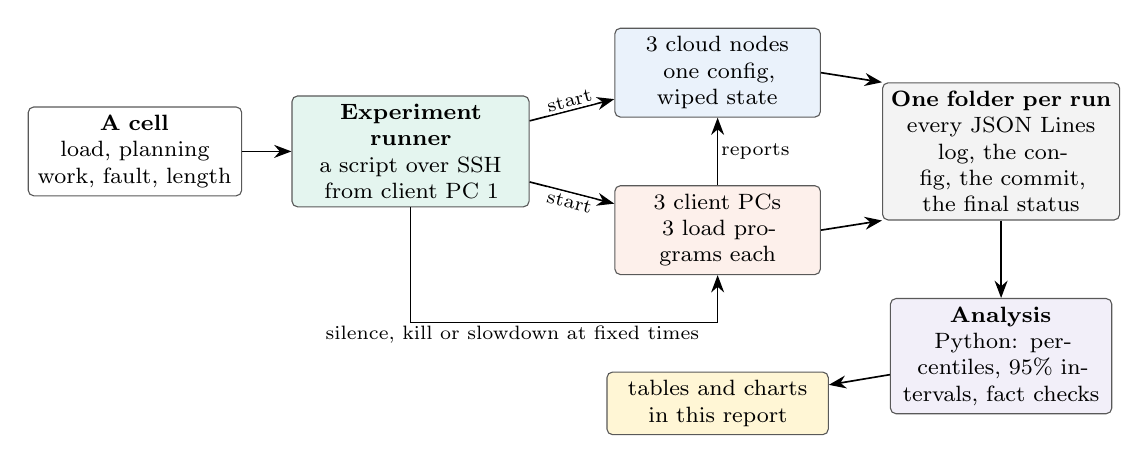
\begin{tikzpicture}[x=1cm,y=1cm, every node/.style={font=\scriptsize}]
  \node[box, fill=white, text width=2.5cm] (cell) at (0,0) {\textbf{A cell}\\ load, planning work, fault, length};
  \node[box, fill=mwgreen!12, text width=2.8cm] (run) at (3.5,0) {\textbf{Experiment runner}\\ a script over SSH from client PC 1};
  \node[nodebox, text width=2.4cm] (nodes) at (7.4,1.0) {3 cloud nodes\\ one config, wiped state};
  \node[clientbox, text width=2.4cm] (clients) at (7.4,-1.0) {3 client PCs\\ 3 load programs each};
  \node[box, fill=libgray!10, text width=2.8cm] (logs) at (11.0,0) {\textbf{One folder per run}\\ every JSON Lines log, the config, the commit, the final status};
  \node[box, fill=apppurple!10, text width=2.6cm] (an) at (11.0,-2.6) {\textbf{Analysis}\\ Python: percentiles, 95\% intervals, fact checks};
  \node[box, fill=notefill, text width=2.6cm] (rep) at (7.4,-3.2) {tables and charts in this report};
  \draw[flow] (cell) -- (run);
  \draw[flow] (run) -- node[elabel, above, sloped]{start} (nodes);
  \draw[flow] (run) -- node[elabel, below, sloped]{start} (clients);
  \draw[flow] (clients) -- node[elabel, right]{reports} (nodes);
  \draw[flow] (run.south) |- node[elabel, pos=0.75, below]{silence, kill or slowdown at fixed times} ($(clients.south west)+(0,-0.6)$) -| (clients.south);
  \draw[flow] (nodes.east) -- (logs.north west);
  \draw[flow] (clients.east) -- (logs.south west);
  \draw[flow] (logs) -- (an);
  \draw[flow] (an) -- (rep);
\end{tikzpicture}
\caption{How an experiment runs. The runner refuses to start if any RescueMesh program is left running on any PC, and marks a run complete only when all its logs are in, so a stopped batch leaves nothing half-counted.}
\label{fig:pipeline}
\end{figure}

\begin{itemize}
  \item \textbf{Design.} The overnight series ran every cell once per pass, then repeated the pass 5 times, so that any drift over the night falls across all cells and not on one. The 5 passes took 6 h 37 min, 5.1 h of it with load running.
  \item \textbf{Load.} Open loop: 9 programs at a fixed rate, 3 on each client PC, evenly spaced, each with its own seed in each pass. Each report goes to all 3 nodes.
  \item \textbf{Settings.} One commit built on all six PCs. 60,000 responders, 20 planning threads, a 60 ms bid window, 1 s detection, the expected-wait score. The CPU energy setting was read at the start of each part and saved with the runs.
  \item \textbf{Measured.} The first 15 s of each run is warm-up and left out. Rates are answers finished per second. Latency is measured on the client's clock with a monotonic timer, from when a report was due to go. Durations are never computed from two machines' clocks; where a figure needs two clocks, the report states how far apart they were, which was 3 to 6 ms.
  \item \textbf{Statistics.} Means across runs with 95\% confidence intervals by Student's $t$; percentiles over all requests of a run. Five runs give wide intervals at the edge of the ceiling, so the run-to-run range is shown there.
  \item \textbf{Runs left out.} The analysis names and leaves out a run with missing programs or logs, a damaged log, or a fault that never fired. Two Scenario 2 cells ran with a script mistake that left the slowed node with no planning work after the slowdown; they are kept and labelled, and the tables use the rerun cells.
\end{itemize}

\textbf{Raw data.} The raw logs are too large to publish, but nothing is deleted: every client's every request, every node's every event, and each run's status and settings are kept on the lab PCs. The per-run and per-cell figures behind every table in this report are published with the project \cite{repo}. Figure~\ref{fig:seq-report} draws one report followed through every PC's log.

% ==============================================================================================
\section{Limits}
\label{sec:limits}

We list what the results do not show, and what the system does not do, as plainly as the results themselves.

\begin{enumerate}
  \item \textbf{No machine was physically turned off.} The professor asked to see this (Oct 28). We used \texttt{kill -9}, which the person running the lab decided is enough (\dlog{D265}). A kill stops the process at once, as a power cut would, but it cannot lose disk writes the way a real cut can.
  \item \textbf{All three killed can lose a few answers.} If nodes return one at a time and the node with the longest log returns last, the others have gone on without its tail, and it starts again from their log. Answers that only it had applied are lost, though the nodes still agree. This happened in 2 of 49 kill runs: 566 of 48,331,376 answers, or 0.0012\%. No run with one or two nodes killed lost any. A fix would have that node hand over its tail first; it is not built.
  \item \textbf{A returning node's file can miss a few batches.} In 5 of 49 kill runs one node's file lacked batches it was handed on return, which it holds in memory but does not save. Its memory and digest matched the others'. If that node restarted again, it would find its log is not a start of the others' and take the log again.
  \item \textbf{Provisional answers usually change.} In T2 with 300 responders, about 98\% of the lone node's answers ended differently on record, and clients are not told. Killing the lone node loses the provisional answers it has not replayed.
  \item \textbf{Memory grows with the log,} about 590 bytes per report per node, and nothing trims it. At 20,000 a second a node runs out after about 18 to 20 minutes; at 1,000 a second it would take about 6.5 hours.
  \item \textbf{A slow patch can feed itself.} Past about 2 s, retries and takeovers plan reports again, which adds load. At 20,000 a second and above this may not recover while the load continues. The retry budget bounds it but does not end it.
  \item \textbf{Results above 15,000 a second depend on the network.} The lab runs on shared, mostly wireless networking. The final build has not been run at 30,000 on a quiet network.
  \item \textbf{A failure costs at least 1 s}, the detection time, since a silent node holds up every round until it is dropped.
  \item \textbf{The planning load is simulated.} \texttt{plan\_work} is a busy loop that stands in for a harder planning job; the real choice of a responder takes microseconds.
  \item \textbf{The ordering is our own code.} Its correctness rests on our tests and these experiments, not on a library's users, and the agreement on a drop has had no formal check.
  \item \textbf{Fewer repeats for some failure runs.} The kill cases have 3 runs at 10,000 a second, 2 at 15,000, and 1 at 20,000 and 300, with random nodes and times.
\end{enumerate}

% ==============================================================================================
\section{What is a library and what is ours}
\label{sec:library}

The spec asks the report to make clear which functions come from libraries and which distributed protocols, election logic, consistency and recovery we designed and built. Table~\ref{tab:library} draws the line. Only two libraries do distributed-systems work: tarpc makes remote calls, and openraft is still compiled in but is off in every lab run (\dlog{D179}, \dlog{D215}).

\begin{table}[!htb]
\centering\small
\caption{Libraries and our own code.}
\label{tab:library}
\begin{tabularx}{\linewidth}{@{}LL@{}}
\toprule
Done by a library & Done by us \\
\midrule
Remote calls, call IDs, deadlines: \texttt{tarpc} 0.37 \cite{tarpc} & The bidding election: \texttt{bidding.rs}, \texttt{node/bids.rs} \\
Async tasks, timers, sockets, file writes: \texttt{tokio} 1 \cite{tokio} & The shared log's order, drop and return: \texttt{rounds.rs} \\
Encoding: \texttt{serde} 1, \texttt{bincode} 1.3 \cite{serde} & The state machine, first result wins, the digest: \texttt{state.rs} \\
Splitting TCP into frames: \texttt{tokio-util} 0.7 & Failure detection and takeover: \texttt{heartbeat.rs}, \texttt{takeover.rs} \\
A socket option for buffers: \texttt{socket2} 0.6 & The fault election and gate; rejoin; the lone node: \texttt{faults.rs}, \texttt{rejoin.rs}, \texttt{degraded.rs} \\
Log lines as JSON: \texttt{serde\_json} & The UDP adapter and compression: \texttt{datagram.rs}, \texttt{squeeze.rs} \\
Raft: \texttt{openraft} 0.9.25 \cite{openraft}, built in but off & The planner; the client middleware with its retries and budget; all experiments and analysis \\
\bottomrule
\end{tabularx}
\end{table}

\textbf{AI and open source.} Much of the code, the tests, the analysis scripts and the first drafts of our documents were written with an AI coding assistant, Claude Code, under the team's direction, as the spec allows. Every design decision was made by a person and recorded with who made it, and the working agreement in \texttt{AGENTS.md} required the assistant to ask about each decision before writing code. All libraries above are open source and used under their licences.

% ==============================================================================================
\section{Phase 2: what comes next}
\label{sec:phase2}

Discovery, presence, peer-to-peer exchange, offline operation and conflicting claims are Phase 2, due on December 5, and none of them is built yet. Our plan builds on what Phase 1 left in place. The discovery directory would be a second state machine on the same shared log: a registration and each lease renewal become commands, so the directory is the same on all three nodes with no new replication protocol (\dlog{D69}). The campus already has zones, which become the topics of a publish-subscribe service: a peer subscribes to the zones it cares about, and incident summaries spread between peers with duplicate suppression by report ID and a hop limit on forwarding (\dlog{D131}, \dlog{D209}). Claims on resources would be leases with fencing tokens, where the token is the claim's position in the shared log, so a late write from an old holder is refused without any node issuing tokens (\dlog{D69}). Offline changes can build on two pieces we already have: answers labelled provisional, and the rule that the first result in the order wins.

% ==============================================================================================
\section{Team contributions}
\label{sec:team}

We worked as one team: decisions were discussed together and written down in the design log, the parts were split for ownership but built to fit one system, and every member can explain the whole of it. For credit, these are the areas each of us mainly built, from the project's history (Table~\ref{tab:team}). The Phase 0 survey was split by algorithm, as its title page shows \cite{survey}.
% CONFIRM: drafted from the git history and the survey's title page. The team should check each row before submitting.

\begin{table}[!htb]
\centering\small
\caption{Main contributions. Everyone also reviewed others' work and took part in the lab sessions they could attend.}
\label{tab:team}
\begin{tabularx}{\linewidth}{@{}P{2.9cm}L@{}}
\toprule
Member & Main contributions \\
\midrule
Noor Emam & Led the design decisions and the lab sessions on the six PCs; the experiment series and final runs; the move to a shared log with no leader and the recovery from several failures; most of the design log and documentation. Survey: Hirschberg-Sinclair. \\
Omar Leithy & Raft and replication on openraft; the state machine, digest and durable log; the client middleware and load generator; tarpc between nodes; the lone node's provisional answers; the first experiment runner and analysis. Survey: ring election. \\
Aabed Elghadban & Fault injection: the fault gate, manual faults and the first fault schedule; the rejoin gate; takeover of a silent winner. Survey: Bully. \\
Ahmed Abdeen & The bidding election: bid rounds, load scores, planning time, and its multi-node tests. Survey: load-aware election. \\
Yahia Kilany & The planner and the seeded campus; the zone penalty; the bounded worker pool. Survey: ZooKeeper Fast Leader Election. \\
Wahiba Elhimer & The transport's reconnect back-off for a peer that is down. Survey: Raft leader election. \\
\bottomrule
\end{tabularx}
\end{table}

% ==============================================================================================
\section{Conclusion}

Phase 1 asked for a cloud of three peers that shares work by an election, survives a node going silent for up to 20 s, rebuilds a returning node's state, and holds up under measured stress. We built that, and the five demonstration scenarios are met on six lab PCs with 0 requests unaccounted for and 0 state mismatches in more than 84,000 comparisons.

The most useful lesson came from changing our mind. The survey's reasons for Raft were sound, and Raft kept every copy correct in every run. But two things only the lab could show made it the wrong fit: its leader is a coordinator in exactly the sense the class rules out, and the leader's one write at a time capped throughput at 7,000 reports a second on the lab's network. Because every part of the node reached the log through one interface, we could replace Raft with a log that has no leader in a day, keep everything above it, and measure both. On the same code at 10,000 reports a second, Raft answered 4,306 a second and rotating rounds answered all of them. The cost is a log that is our own code, a failover that waits for detection, and the work it took to survive two and three failures, which we have measured and listed.

The second lesson is that the network shapes everything. Our timers, the bid window, the packet sizes and even the ceiling were all set by what the lab's shared Wi-Fi could carry, and none of it showed up on one PC. We expect the same to hold in Phase 2, when the peers start talking to each other directly.


\newpage
\begin{thebibliography}{99}
\addcontentsline{toc}{section}{References}
\small

\bibitem{spec} A.~El-Kadi. \emph{RescueMesh: A Cloud-P2P Environment for Smart-Campus Emergency Response and Resource Coordination}. CSCE 4411 term project description, The American University in Cairo, Fall 2026.

\bibitem{notes} Class notes on the project, CSCE 4411, Fall 2026: Sept 6, Sept 9, Sept 13, Oct 4 and Oct 28.

\bibitem{survey} A.~Elghadban, O.~Leithy, N.~Emam, W.~Elhimer, A.~Abdeen and Y.~Kilany. \emph{Distributed Election Algorithms Survey: RescueMesh}. CSCE 4411 Phase 0 deliverable, October 4, 2026.

\bibitem{repo} The RescueMesh team. \emph{RescueMesh source code, design log and results}. \url{https://github.com/noortaytoy1/DistributedSystems}. The documents cited here are in its \texttt{docs/} folder: \texttt{design-log.md} (decisions D1 to D266), \texttt{architecture.md}, \texttt{shared-log.md}, \texttt{protocol.md}, \texttt{requirements-check.md}, \texttt{phase1-report.md}, \texttt{runbook.md} and \texttt{demo.md}. The results are in \texttt{analysis/results/}, with \texttt{RESULTS.md} as the record of the Raft-era runs.

\bibitem{coulouris} G.~Coulouris, J.~Dollimore, T.~Kindberg and G.~Blair. \emph{Distributed Systems: Concepts and Design}, 5th ed. Addison-Wesley, 2012.

\bibitem{raft} D.~Ongaro and J.~Ousterhout. In search of an understandable consensus algorithm. In \emph{Proc.\ USENIX ATC}, 2014, pp.~305--319.

\bibitem{lamport} L.~Lamport. Time, clocks, and the ordering of events in a distributed system. \emph{Communications of the ACM}, 21(7):558--565, 1978.

\bibitem{garcia} H.~Garcia-Molina. Elections in a distributed computing system. \emph{IEEE Transactions on Computers}, C-31(1):48--59, 1982.

\bibitem{contractnet} R.~G.~Smith. The contract net protocol: high-level communication and control in a distributed problem solver. \emph{IEEE Transactions on Computers}, C-29(12):1104--1113, 1980.

\bibitem{chandra} T.~D.~Chandra and S.~Toueg. Unreliable failure detectors for reliable distributed systems. \emph{Journal of the ACM}, 43(2):225--267, 1996.

\bibitem{jain} R.~Jain, D.-M.~Chiu and W.~Hawe. A quantitative measure of fairness and discrimination for resource allocation in shared computer systems. DEC Technical Report TR-301, 1984.

\bibitem{openraft} openraft 0.9.25, a Raft library for Rust. \url{https://crates.io/crates/openraft}.

\bibitem{tarpc} tarpc 0.37, an RPC framework for Rust. \url{https://crates.io/crates/tarpc}.

\bibitem{tokio} tokio 1, an asynchronous runtime for Rust. \url{https://tokio.rs}.

\bibitem{serde} serde 1 and bincode 1.3, serialization for Rust. \url{https://serde.rs}, \url{https://crates.io/crates/bincode}.

\bibitem{lz4} Y.~Collet. LZ4 block format description. \url{https://github.com/lz4/lz4/blob/dev/doc/lz4_Block_format.md}.

\bibitem{claude} Anthropic. \emph{Claude Code}, with the Claude Opus models. An AI coding assistant, used under the team's direction to write code, tests, analysis scripts and drafts of the documentation. \url{https://claude.com/claude-code}, 2026.

\end{thebibliography}

\end{document}
